% 11/23/2015
%%%%%%%%%%%%%%%%%%%%%%%%%%%%%%%%%%%%%%%%%%%%%%%%%%%%%%%%%%%%%%%%%%%%%%%%%%%%
% AGUJournalTemplate.tex: this template file is for articles formatted with LaTeX
%
% This file includes commands and instructions
% given in the order necessary to produce a final output that will
% satisfy AGU requirements. 
%
% You may copy this file and give it your
% article name, and enter your text.
%
%%%%%%%%%%%%%%%%%%%%%%%%%%%%%%%%%%%%%%%%%%%%%%%%%%%%%%%%%%%%%%%%%%%%%%%%%%%%
% PLEASE DO NOT USE YOUR OWN MACROS
% DO NOT USE \newcommand, \renewcommand, or \def, etc.
%
% FOR FIGURES, DO NOT USE \psfrag or \subfigure.
% DO NOT USE \psfrag or \subfigure commands.
%%%%%%%%%%%%%%%%%%%%%%%%%%%%%%%%%%%%%%%%%%%%%%%%%%%%%%%%%%%%%%%%%%%%%%%%%%%%
%
% All questions should be e-mailed to latex@agu.org.
%
%%%%%%%%%%%%%%%%%%%%%%%%%%%%%%%%%%%%%%%%%%%%%%%%%%%%%%%%%%%%%%%%%%%%%%%%%%%%
%
% Step 1: Set the \documentclass
%
% There are two options for article format:
%
% 1) PLEASE USE THE DRAFT OPTION TO SUBMIT YOUR PAPERS.
% The draft option produces double spaced output.
% 
% 2) numberline will give you line numbers.

%% To submit your paper:
%\documentclass[draft,linenumbers]{agujournal}
%\draftfalse

%% For final version.
\documentclass{agujournal}
\usepackage{url}
% Now, type in the journal name: \journalname{<Journal Name>}

% ie, \journalname{Journal of Geophysical Research}
%% Choose from this list of Journals:
%
% JGR-Atmospheres
% JGR-Biogeosciences
% JGR-Earth Surface
% JGR-Oceans
% JGR-Planets
% JGR-Solid Earth
% JGR-Space Physics
% Global Biochemical Cycles
% Geophysical Research Letters
% Paleoceanography
% Radio Science
% Reviews of Geophysics
% Tectonics
% Space Weather
% Water Resource Research
% Geochemistry, Geophysics, Geosystems
% Journal of Advances in Modeling Earth Systems (JAMES)
% Earth's Future
% Earth and Space Science
%
%

\journalname{Journal of Advances in Modeling Earth Systems (JAMES)}


\begin{document}

%% ------------------------------------------------------------------------ %%
%  Title
% 
% (A title should be specific, informative, and brief. Use
% abbreviations only if they are defined in the abstract. Titles that
% start with general keywords then specific terms are optimized in
% searches)
%
%% ------------------------------------------------------------------------ %%

% Example: \title{This is a test title}

\title{NCAR CESM2.0 release of CAM-SE: A reformulation of the spectral-element dynamical core in dry-mass vertical coordinates with comprehensive treatment of condensates and energy}

%% ------------------------------------------------------------------------ %%
%
%  AUTHORS AND AFFILIATIONS
%
%% ------------------------------------------------------------------------ %%

% Authors are individuals who have significantly contributed to the
% research and preparation of the article. Group authors are allowed, if
% each author in the group is separately identified in an appendix.)

% List authors by first name or initial followed by last name and
% separated by commas. Use \affil{} to number affiliations, and
% \thanks{} for author notes.  
% Additional author notes should be indicated with \thanks{} (for
% example, for current addresses). 

% Example: \authors{A. B. Author\affil{1}\thanks{Current address, Antartica}, B. C. Author\affil{2,3}, and D. E.
% Author\affil{3,4}\thanks{Also funded by Monsanto.}}

\authors{P.H. Lauritzen\affil{1}\thanks{1850 Table Mesa Drive, Boulder, Colodaro, USA}, R.D. Nair\affil{1}, A.R. Herrington\affil{2},P. Callaghan\affil{1}, S. Goldhaber\affil{1}, J.M. Dennis\affil{1}, J.T. Bacmeister\affil{1}, B.E. Eaton\affil{1}, C.M. Zarzycki\affil{1}, Mark A. Taylor\affil{3}, P.A. Ullrich\affil{4}, T. Dubos\affil{5}, A. Gettelman\affil{1},  R.B. Neale\affil{1}, B. Dobbins\affil{1}, K.A. Reed\affil{2}, C. Hannay\affil{1}, B. Medeiros\affil{1}, J.J. Benedict and J.J. Tribbia\affil{1}}

 \affiliation{1}{National Center for Atmospheric Research, Boulder, Colorado, USA}
 \affiliation{2}{School of Marine and Atmospheric Sciences, Stony Brook University, State University of New York, Stony Brook, New York}
 \affiliation{3}{Sandia National Laboratories, Albuquerque, New Mexico, USA}
 \affiliation{4}{Department of Land, Air and Water Resources, University of California, Davis, California, USA}
 \affiliation{5}{Ecole Polytechnique, UMR 8539, Laboratoire de M\'et\'eorologie Dynamique/IPSL, Palaiseau, France}
 \affiliation{6}{Rosenstiel School of Marine and Atmospheric Science, University of Miami, Miami, Florida, USA}

% \affiliation{3}{Third Affiliation}
% \affiliation{4}{Fourth Affiliation}

%(repeat as many times as is necessary)

%% Corresponding Author:
% Corresponding author mailing address and e-mail address:

% (include name and email addresses of the corresponding author.  More
% than one corresponding author is allowed in this LaTeX file and for
% publication; but only one corresponding author is allowed in our
% editorial system.)  

% Example: \correspondingauthor{First and Last Name}{email@address.edu}

\correspondingauthor{peter Hjort Lauritzen}{pel@ucar.edu}

%% Keypoints, final entry on title page.

% Example: 
% \begin{keypoints}
% \item	List up to three key points (at least one is required)
% \item	Key Points summarize the main points and conclusions of the article
% \item	Each must be 100 characters or less with no special characters or punctuation 
% \end{keypoints}

%  List up to three key points (at least one is required)
%  Key Points summarize the main points and conclusions of the article
%  Each must be 100 characters or less with no special characters or punctuation 

\begin{keypoints}
\item The CESM2.0 release of the spectral-element dynamical core (CAM-SE) is documented
\item Model has comprehensive treatment of condensates and energy
\item The CAM-SE model has been sped-up significantly compared to its predecessor CAM-HOMME
\end{keypoints}

%% ------------------------------------------------------------------------ %%
%
%  ABSTRACT
%
% A good abstract will begin with a short description of the problem
% being addressed, briefly describe the new data or analyses, then
% briefly states the main conclusion(s) and how they are supported and
% uncertainties. 
%% ------------------------------------------------------------------------ %%

%% \begin{abstract} starts the second page 

\begin{abstract}
It is the purpose of this paper to provide a comprehensive documentation of the new NCAR version of the spectral-element (SE) dynamical core as part of the CESM2.0 release. This version differs from previous releases of the SE dynamical core in several ways. Most notably the hybrid-sigma vertical coordinate is based on dry air mass, the condensates are dynamically active in the thermodynamic and momentum equations (also referred to as condensate loading), and the continuous equations of motion conserve a more comprehensive total energy that includes condensates. The code base has been significantly reduced, sped-up, and cleaned up as part of integrating SE as a dynamical core in the CAM (Community Atmosphere Model) repository rather than importing the SE dynamical core from HOMME (High-Order Method Modeling Environment) as an external code.
\end{abstract}


%% ------------------------------------------------------------------------ %%
%
%  TEXT
%
%% ------------------------------------------------------------------------ %%

%%% Suggested section heads:
%\section{Introduction}
% 
% The main text should start with an introduction. Except for short
% manuscripts (such as comments and replies), the text should be divided
% into sections, each with its own heading. 

% Headings should be sentence fragments and do not begin with a
% lowercase letter or number. Examples of good headings are:

% \section{Materials and Methods}
% Here is text on Materials and Methods.
%
% \subsection{A descriptive heading about methods}
% More about Methods.
% 
% \section{Data} (Or section title might be a descriptive heading about data)
% 
% \section{Results} (Or section title might be a descriptive heading about the
% results)
% 
% \section{Conclusions}


\section{Introduction}
Over the last two decades or so, the spectral-element (SE) method has been considered as a numerical method for the fluid flow solver in  global weather/climate models \citep{FT2004MWR,BWTF2006MWR,KG2012JCP,GKC2013SIAM,CH2016APJAS}. The main motivations were the SE methods' near perfect scalability \citep{DetAl2012IJHPCA}, GPU acceleration \citep[e.g.][]{AWWGIJHPCA,AetAl2017IJHPCA}, high-order accuracy for smooth problems, and mesh-refinement capabilities. For some time the Community Earth System Model \citep[CESM; ][]{CESM1} has supported a SE dynamical core option in the atmosphere component CAM \citep[Community Atmosphere Model; ][]{CAM5} discretized on a cubed-sphere grid (Figure \ref{fig:grids}a). The SE dynamical core in CAM supports uniform resolution grids based on the equi-angular gnomonic cubed-sphere grid \citep{RP1996QJ} as well as a mesh-refinement capability with local increases in resolution through conformal mesh-refinement as shown on Figure \ref{fig:grids}b {\citep{FT2004MWR,BWTF2006MWR,ZetAl2014JC,ZetAl2014JCb}. The dynamical core code resided in the High-Order Methods Modeling environment (HOMME), a framework for developing new generation computationally efficient and petascale capable dynamical cores based on the SE method \citep{TL2000JSC,TES2008JPCS}, the discontinuous Galerkin method \citep{NCT2009CF} and finite-volume method \citep{ELGT2012PCS,LTOUNGK2017MWR}. Previously, the SE dynamical core was imported into CAM as an external code base. Consequently any updates to the HOMME code base would have to be imported into CAM and pass regression tests in both HOMME and CAM. We refer to this setup as CAM-HOMME, which has been extensively tested in AMIP-style climate simulations \citep[e.g., ][]{ELMNTT2012JC,ZJ2014JAMES,RetAl2015GRL,BetAl2016CC,RHUZ2016JAMC,GetAl2017JAMES}. CAM-SE's code base is in CAM and not HOMME. CAM-SE and HOMME codes have diverged significantly due to a  massive code clean-up to satisfy software engineering standards in CAM (and make the code more user-friendly for the community) as well as considerable science changes described herein.
  \begin{figure}[h]
\centering
 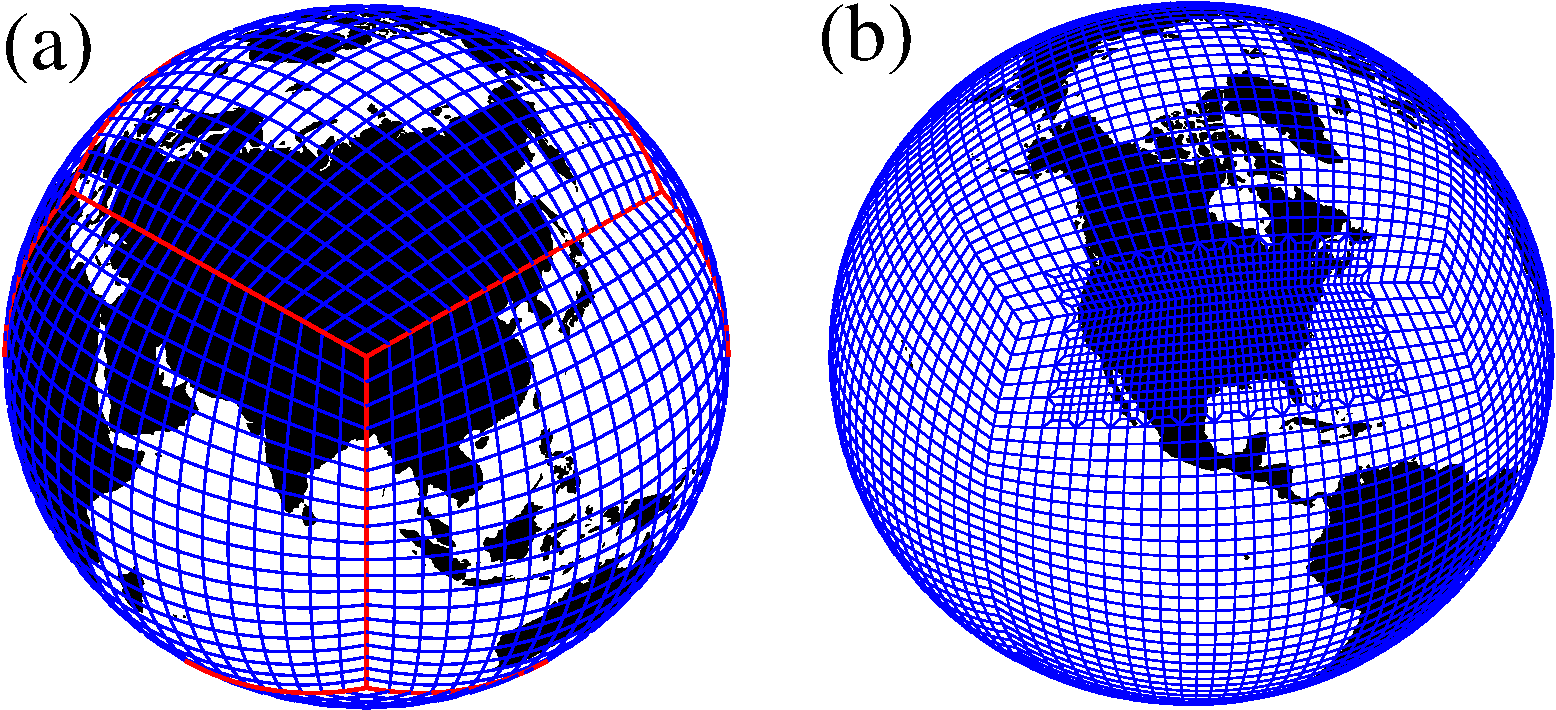
\includegraphics[scale=0.45]{figs/grids}
 \caption{(a) The gnomonic equi-angular cubed-sphere grid that define the elements in CAM-SE. (b) Elements of a conformal mesh-refinement grid referred to as the CONUS-grid (Contiguous United States) used in CAM-SE.}
 \label{fig:grids}
\end{figure}


In this paper we present a version of the SE dynamical core using a dry-mass vertical coordinate that includes condensate-loading, and the continuous equations of motion conserve a comprehensive moist total energy containing all prognostic water variables and their respective heat capacities in the thermodynamic equation. {\color{red}{The basic spectral-element method has not been changed but we present changes to the details of how hyperviscosity is applied and the vertical remapping that are not specific to the dry-mass vertical coordinate.}} As this paper serves as documentation for the CESM2.0 version of SE we also provide details on the spectral-element method and viscosity operators that have not been comprehensively documented in previous publications. 

The SE dynamical core is the default dynamical core for high-resolution CESM applications, in particular, the configuration in which the average distance between grid-points is approximately ~28km \citep{BetAl2016CC}. At such resolutions the effects of condensates (such as cloud liquid and rain) may have a significant effect on the dynamics \citep{BLDT2012GRL}. CAM-HOMME does not represent the effect of condensates in the thermodynamic and momentum equations (also referred to as condensate loading). Including the thermodynamic and mass effect of condensates in the dynamical core is easier when using a dry-mass hybrid-sigma vertical coordinate than when using the usual moist-mass hybrid-sigma vertical coordinate \citep[e.g., ][]{SB1981MWR}. This is the initial motivation for using a dry-mass vertical coordinate.

A second motivation for switching to a dry-mass vertical coordinate is the consistent coupling with the physical parameterizations. CAM physics assumes that the (moist) pressure levels are constant during the parameterization updates. Consequently the moist pressure levels stay constant even when moisture leaves the column (e.g., rains out). At the very end of CAM physics the change in water  vapor in each column is taken into account by scaling the mixing ratios for all tracers that are based on specific/moist mixing ratios so that dry air mass and tracer mass is conserved \citep[see Section 3.1.6 in ][]{CAM5}. This scaling does not guarantee shape-preservation and changes the total energy. In addition, the pressure field in CAM physics does not take into account the mass of condensates. When using a dry-mass vertical coordinate, the coordinate surfaces (assuming dry mass is constant) remain constant throughout the physics updates and there is no need to adjust tracer mixing ratios, and one can more rigorously take into account the work performed by water variables in the context of the energy cycle.

The third motivation for using a dry-mass vertical coordinate relates to total energy conservation. Currently the energy fixer in CAM is based on a dry total energy \citep{WOHTTV2015JAMES} that uses the same heat-capacity for dry air and water vapor, and does not include the effect of condensates. To move towards a more accurate treatment of energy in CAM, a first step is to develop a dynamical core based on equations of motion conserving an energy that more accurately represents water vapor as well as condensates. This is most easily done when using a dry-mass vertical coordinate so that the energies associates with all water variables are clearly separated. Similarly for axial angular momentum (AAM) which is an important conserved quantity of the continuous equations of motion \citep[e.g., ][]{LHECFF2010JGR}.

The paper is organized as follows. In section \ref{sec:cont-eq} the continuous equations of motion are derived which involves a detailed discussion of moist thermodynamics in the presence of condensates. The AAM and total energy conservation properties of continuous system of equations is also discussed. In section \ref{sec:discretized_eqs} the discretized equations of motion with focus on the vertical discretization in dry-mass vertical coordinates are derived. Details on the horizontal SE discretization on the cubed-sphere are also presented. Section \ref{sec:results} presents some results, validating the new dynamical core in idealized configurations. First, a moist baroclinic wave with simple warm-rain micro-physics and secondly in a CAM6{\footnote{the CAM6 physics tag is {\tt{cam5\_4\_128}} which is a near final pre-release version of the CESM2.0-CAM6 physics package; this paper focuses on the dynamical core and the details of the physics package are less important}} aqua-planet configuration. The computational performance of CAM-SE is presented in section \ref{sec:results}. The paper ends with summary and conclusions in section \ref{sec:concl}.
%
\section{Continuous equations}\label{sec:cont-eq}
Before writing the continuous equations of motion using a dry-mass vertical coordinate (section \ref{eq:eqnsmotion}), we first need to discuss the representation of water variables (section \ref{sec:mixing_ratios}), discuss the ideal gas law (section \ref{sec:tv}) and derive the thermodynamic equation for a mixture containing all water species (section \ref{sec:teqn}). The discussion of the equations of motion in the presence of water vapor, cloud liquid, ice, rain and snow closely follows \citet{joyOfUM}. {\color{red}{While the appropriate thermodynamics of moist air is well-understood \citep[e.g.][]{E1994} it is unclear how to best represent moist dynamical effects in numerical models \citep{O1990JAS,O2001MWR,S2003MWR,B2003JAS}.}}  Therefore the derivation of the equations of motion including non-gas components is discussed in detail.

%As noted in \cite{cotton2010storm} ' ... the fundamental equations governing dry air are generally accepted in fluid dynamics communities. By contrast, the governing equations for moist atmosphere flows remain a source of some controversy and active research'.




Thereafter the dry mass vertical coordinate is defined in section \ref{eq:vertical_coord}. Details on viscosity and frictional heating are presented in section \ref{sec:hypvervisfric} and global conservation properties derived in section \ref{sec:aam}.
\subsection{Representation of water phases in terms of dry and wet (specific) mixing ratios}\label{sec:mixing_ratios}
{\color{red}{Equation \eqref{eq:mx} defines}} the dry mixing ratios for the water variables (vapor 'wv', cloud liquid 'cl', cloud ice 'ci', rain 'rn' and snow 'sw')
\begin{equation}
m^{(\ell)}\equiv \frac{\rho^{(\ell)}}{\rho^{(d)}}, \text{ where }\ell=`wv`,`cl`,`ci`,`rn`,`sw`,\label{eq:mx}
\end{equation}
where $\rho^{(d)}$ is the mass of dry air per unit volume of moist air and $\rho^{(\ell)}$ is the mass of the water substance of type $\ell$ per unit volume of moist air. Note that the mixing ratio for dry air is unity: $m^{(d)}\equiv \frac{\rho^{(d)}}{\rho^{(d)}}=1$. 
Moist air refers to air containing dry air, water vapor, cloud liquid, cloud ice, rain amount and snow amount. For notational purposes define the set of all components of air
\begin{equation}
\mathcal{L}_{all}=\left\{ `d`,`wv`,`cl`,`ci`,`rn`,`sw`\right\},
\end{equation}
a set only referring to all water variables,
\begin{equation}
\mathcal{L}_{water}=\left\{`wv`,`cl`,`ci`,`rn`,`sw`\right\},
\end{equation}
and a set referring to all condensates (non-gas components of water)
\begin{equation}
\mathcal{L}_{cond}=\left\{`cl`,`ci`,`rn`,`sw`\right\}.
\end{equation}
The density of a unit volume of moist air is related to the dry air density through
\begin{equation}
\label{eq:rhosum}
\rho=\rho^{(d)}\left(\sum_{\ell \in \mathcal{L}_{all}} m^{(\ell)}\right).
\end{equation}
Mixing ratios can also be specified in terms of density per density of moist air, in other words, specific/moist mixing ratios
\begin{equation}
q^{(\ell)}\equiv \frac{\rho^{(\ell)}}{\rho},\label{eq:qx}
\end{equation}
where, in particular, $q^{(wv)}$ is the specific humidity. 


It is straight forward to convert between moist and dry mixing ratios
\begin{align}
m^{(\ell)}&=\frac{q^{(\ell)}}{1-\sum_{\ell \in \mathcal{L}_{water}} q^{(\ell)}},\label{eq:mxqx}\\
q^{(\ell)}&=\frac{m^{(\ell)}}{\sum_{\ell \in \mathcal{L}_{all}} m^{(\ell)}}.
\end{align}
Note that if water vapor undergoes a phase change to rain and leaves the column, then the specific/wet mixing ratios change but the dry mixing ratios do not.
%
\subsection{Ideal gas law and virtual temperature}\label{sec:tv}
%In this section, the ideal gas law is derived for moist air containing condensates. In a parcel of moist air
%of volume $V$, the condensed phases occupy volumes $V^{(\ell)}$ with $\ell \in \mathcal{L}_{cond}$. Dry air and pure water vapor are
%assumed to be ideal perfect gases, and the gaseous part of moist air is assumed to be a perfect mixture of
%those gases. Therefore it is possible to assign a volume $V^{(d)}$ to dry air and $V^{(wv)}$ to water vapor, in proportion
%to their respective number of molecules. The total volume is $V=\sum_{\ell \in \mathcal{L}_{all}}V^{(\ell)}$. Now let 
%\begin{equation}
%\alpha^{(\ell)}\equiv \frac{V^{(\ell)}}{V\, \rho^{(\ell)}},
%\end{equation}
%be the specific volume of each phase or component considered separately, let
%\begin{equation}
%\alpha^{(gas)}\equiv \frac{ V^{(d)} + V^{(wv)}}{V \left( \rho^{(d)} + \rho^{(wv)}\right)},
%\end{equation}
%be the specific volume of the gaseous phase considered separately from the condensed phases, and let
%\begin{equation}
%\alpha\equiv \frac{1}{\rho},\label{eq:rhoalpha}
%\end{equation}
%be the total specific volume. Also, note that
%\begin{equation}
%\label{eq:sum1}
%1 = \sum_{\ell \in \mathcal{L}_{(all)}} \rho^{(\ell)}\alpha^{(\ell)} = \alpha^{(gas)}\rho^{(gas)} + \sum_{\ell \in \mathcal{L}_{cond}}\rho^{(\ell)}\alpha^{(\ell)}.
%\end{equation}

In this section, the ideal gas law is derived for moist air containing condensates. In a parcel of moist air
of volume $V$, the gaseous components of moist air (dry air and water vapor) occupy volume $V^{(gas)}$ and the the condensed phases occupy volume $V^{(cond)}=V-V^{(gas)}$. The ideal gas law applies to the gaseous component of air only. In that case, the partial pressure of dry air (the pressure dry air would exert if it alone would occupy the volume)
\begin{equation}
p^{(d)}V^{(gas)}=N^{(d)}k_B T,
\end{equation}
where $k_B$ is the Boltzmann constant and $N^{(d)}$ is the number of molecules of dry air. Now
\begin{equation}
N^{(d)}=\frac{V \rho^{(d)}}{\mathcal{M}^{(d)}},
\end{equation}
where $\mathcal{M}^{(d)}$ is the molar mass of dry air, so the ideal gas law for the partial pressure of dry air can be written as
\begin{equation}
p^{(d)}V^{(gas)}=V\rho^{(d)}R^{(d)}T,
\end{equation}
where $R^{(d)}\equiv \frac{k_B}{\mathcal{M}^{(d)}}$ is the dry air gas constant. Similarly for the partial pressure of water vapor:
\begin{equation}
p^{(wv)}V^{(gas)}=V\rho^{(vw)}R^{(vw)}T,
\end{equation}
where $R^{(wv)}\equiv \frac{k_B}{\mathcal{M}^{(wv)}}$ is the gas constant for water vapor. According to Dalton's law of partial pressures, the total pressure exerted is equal to the sum of the partial pressures of the individual gases:
\begin{equation}
\label{eq:ptmp}
p=\frac{V}{V^{(gas)}}\left( \rho^{(d)}R^{(d)}T+\rho^{(wv)}R^{(wv)}T\right).
\end{equation}
Note that the condensates do not exert a gas pressure ({\color{red}{see}} Section \ref{sec:dryairp}). Moving $T$, $R^{(d)}$ and $\rho^{(d)}$ outside the parenthesis on the right-hand side of \eqref{eq:ptmp} yields
\begin{equation}
\label{eq:ptmp2}
p=\frac{V}{V^{(gas)}}\rho^{(d)}R^{(d)}\left( 1+\frac{1}{\epsilon}m^{(wv)}\right)T,
\end{equation}
where $\epsilon\equiv \frac{R^{(d)}}{R^{(wv)}}$. Multiplying \eqref{eq:ptmp2} with $\rho/\rho$ and simplifying using \eqref{eq:mx}, and \eqref{eq:rhosum} yields
\begin{equation}
\label{eq:ptmp3}
p=\frac{V}{V^{(gas)}}\rho R^{(d)}\left(\frac{ 1+\frac{1}{\epsilon}m^{(wv)}}{\sum_{\ell \in \mathcal{L}_{all}}m^{(\ell)}}\right)T,
\end{equation}
By defining the virtual temperature
\begin{equation}
T_v =T\left( \frac{1+\frac{1}{\epsilon}m^{(wv)}}{\sum_{\ell \in \mathcal{L}_{all}}m^{(\ell)}}\right),\label{eq:tv}
\end{equation}
and assuming that the volume of the condensates is zero $V=V^{(gas)}$ then \eqref{eq:ptmp3} can be written as
\begin{equation}
p=\rho R^{(d)} T_v\label{eq:igl}.
\end{equation}
%
%Now $\rho^{(\ell)}\alpha^{(\ell)}$ is the volume fraction $\frac{V^{(\ell)}}{V}$, especially:
%\begin{equation}
%\rho^{(gas)}\alpha^{(gas)}=\frac{V^{(gas)}}{V}.\label{eq:rhogas}
%\end{equation}
%Consequently, by substituting \eqref{eq:rhogas} into \eqref{eq:ptmp}, using \eqref{eq:mx} to write density in terms of mixing ratio, and simplifying yields
%\begin{equation}
%p=\rho^{(d)}\frac{R^{(d)} T\left( 1+\frac{1}{\epsilon}m^{(wv)}\right)}{\rho^{(gas)}\alpha^{(gas)}}\label{eq:ig3},
%\end{equation}
%where $\epsilon\equiv \frac{R^{(d)}}{R^{(wv)}}$. Using \eqref{eq:sum1} to eliminate $\rho^{(gas)}\alpha^{(gas)}$ in \eqref{eq:ig3}, 
%Multiplying by $\frac{\rho}{\rho}$, and manipulating the denominator using \eqref{eq:mx}, and \eqref{eq:rhosum}, and simplifying  yields 
%
%where the virtual temperature is given by
%\begin{equation}
%T_v =T\left[ \frac{1+\frac{1}{\epsilon}m^{(wv)}}{1+m^{(wv)}+\sum_{\ell\in \mathcal{L}_{cond}}m^{(\ell)}\left(1-\frac{\alpha^{(\ell)}}{\alpha}\right)}\right].
%\end{equation}
%The ratios of the specific volume of the condensates to the total specific volume of moist air are negligible (e.g., the terms $\frac{\alpha^{(\ell)}}{\alpha}$ are of order $10^{-3}$ or less) hence the formula for virtual temperature is simplified to
%\begin{equation}
%T_v =T\left( \frac{1+\frac{1}{\epsilon}m^{(wv)}}{\sum_{\ell \in \mathcal{L}_{all}}m^{(\ell)}}\right), \text{ if } V^{(\ell)}=0 \text{ for }\ell \in \mathcal{L}_{cond}.\label{eq:tv}
%\end{equation}


%Even though the density of condensates can be $10^{3}$ larger than the density of the gaseous components of air, the fraction of a unit volume occupied by the condensates is negligible, i.e. $\alpha^{(gas)}\rho^{(gas)} \ll \sum_{\ell \in \mathcal{L}_{cond}}\rho^{(\ell)}\alpha^{(\ell)}$. Henceforth we assume that 
%\begin{equation}
%V^{(\ell)}=0, \text{ for }\ell \in \mathcal{L}_{cond}.
%\end{equation}
%Using Dalton's law of partial pressures,  the total gas pressure is the sum of the partial pressure of dry air (the pressure dry air would exert if it alone would occupy the volume) and the partial pressure of water vapor
%\begin{equation}
%p=p^{(d)}+p^{(wv)},\label{eq:ig} %=\rho^{(d)} R^{(d)} T+\rho^{(wv)} R^{(wv)} T
%\end{equation}
%The ideal gas law for dry air is


%e may write \eqref{eq:ig} in terms of $\rho^{(gas)}$ by multiplying \eqref{eq:ig} with $\frac{\rho^{(gas)}}{\rho^{(gas)}}$ and write the equation in terms of mixing ratios


%In this section the ideal gas law is derived for moist air containing condensates. Part of that derivation is the definition of virtual temperature. A unit volume of moist air $V=1$ is the sum of the volume of dry air and the volumes of the different forms of water in the air
%\begin{equation}
%V=\sum_{\ell \in \mathcal{L}_{all}} V^{(\ell)}.\label{eq:Volumes}
%\end{equation}
%Now let $\alpha\equiv \frac{1}{\rho}$ denote the specific volume of moist air, let $\alpha^{(gas)}$ be the specific volume of the gaseous components of moist air (the volume of water vapor and dry air per unit mass of water vapor and dry air), let $\alpha^{(cl)}$ be the specific volume of cloud liquid (i.e. volume occupied by unit mass of cloud liquid), and similarly for cloud ice, rain and snow. Then we can write \eqref{eq:Volumes} in terms of densities and specific volumes
%\begin{equation}
%\rho \alpha=\rho^{(gas)}\alpha^{(gas)}+\sum_{\ell\in \mathcal{L}_{cond}}\rho^{(\ell)}\alpha^{(\ell)},\label{eq:massV}
%\end{equation}
%where $\rho^{(gas)}=\rho^{(d)}+\rho^{(wv)}$. Note that $\alpha^{(\ell)}\neq \frac{1}{\rho^{(\ell)}}$ since $\rho^{(\ell)}$ is defined in terms mass of $\ell$ per unit volume of moist air and not mass of $\ell$ per unit volume of water phase $\ell$. Dividing \eqref{eq:massV} with $\rho^{(d)}$ and substituting \eqref{eq:mx} yields
%\begin{equation}
%  \left(\sum_\ell m^{(\ell)}\right) \alpha = \left( 1+m^{(wv)}\right) \alpha^{(gas)}+\sum_{\ell\in \mathcal{L}_{cond}}m^{(\ell)}\alpha^{(\ell)}.\label{eq:vol}
%\end{equation}
%The ideal gas law for the gaseous components, using Dalton's law of partial pressures, is
%\begin{equation}
%p=p^{(d)}+p^{(wv)}=\rho^{(d)} R^{(d)} T+\rho^{(wv)} R^{(wv)} T,\label{eq:ig}
%\end{equation}
%where $p^{(d)}$ is the partial pressure exerted by dry air (the pressure dry air would exert if it alone would occupy the volume) and $p^{(wv)}$ is the partial pressure of water vapor (again, the pressure exerted by water vapor if it alone would occupy the volume). Note that the condensates do not exert a gas pressure (more in this in Section \ref{sec:dryairp}). We may write \eqref{eq:ig} in terms of $\rho^{(gas)}$ by multiplying \eqref{eq:ig} with $\frac{\rho^{(gas)}}{\rho^{(gas)}}$ and write the equation in terms of mixing ratios
%\begin{equation}
%p=R^{(d)} T\rho^{(gas)}\left( \frac{\rho^{(d)}}{\rho^{(gas)}}+\frac{\rho^{(wv)}}{\rho^{(gas)}}\frac{R^{(wv)}}{R^{(d)}}\right)=\frac{R^{(d)} \rho^{(gas)}T\left( 1+\frac{1}{\epsilon}m^{(wv)}\right)}{\left(1+m^{(wv)}\right)}\label{eq:ig2}.
%\end{equation}
%where . Since \eqref{eq:ig} holds for the gaseous components only we may substitute $\frac{1}{\rho^{(gas)}}$ with $\alpha^{(gas)}$ to get:

\subsection{Thermodynamic equation}\label{sec:teqn}
Let $S$ denote the total entropy of moist air
\begin{equation}
S=\sum_{\ell \in \mathcal{L}_{all}}S^{(\ell)},
\end{equation}
where $S^{(\ell)}$ is the entropy of component $\ell$ of moist air. From the chain rule applied to each component separately we get
\begin{align}
dS&=\sum_{\ell \in \mathcal{L}_{all}}dS^{(\ell)},\\
  &=\sum_{\ell \in \mathcal{L}_{all}}\left[ \frac{\partial S^{(\ell)}}{\partial E^{(\ell)}}dE^{(\ell)}+\frac{\partial S^{(\ell)}}{\partial V^{(\ell)}}dV^{(\ell)}\right],\label{eq:dS1}
\end{align}
where $V^{(\ell)}$ is the volume occupied by component $\ell$ of moist air and $E^{(\ell)}$ is the internal energy of $\ell$. If we assume that the condensates are incompressible, $dV^{(\ell)}=0$ for $\ell \in \mathcal{L}_{cond}$, then  \eqref{eq:dS1} becomes
\begin{equation}
dS  =\sum_{\ell \in \mathcal{L}_{all}}\frac{\partial S^{(\ell)}}{\partial E^{(\ell)}}dE^{(\ell)}+\sum_{\ell \in \mathcal{L}_{gas}}\frac{\partial S^{(\ell)}}{\partial V^{(\ell)}}dV^{(\ell)}.\label{eq:dS2}
\end{equation}
Using that $\frac{\partial S^{(\ell)}}{\partial V^{(\ell)}}=\frac{p^{(\ell)}}{T}$ for $\ell \in \mathcal{L}_{gas}$, {\color{red}{$\frac{\partial S^{(\ell)}}{\partial E^{(\ell)}} = \frac{1}{T}$}} and that
\begin{equation}
dE^{(\ell)}=C_v^{(\ell)}dT,
\end{equation}
where $C_v^{(\ell)}$ is the heat capacity of $\ell$ at constant volume, then \eqref{eq:dS2} can be written as
\begin{equation}
\sum_{\ell \in \mathcal{L}_{all}}C_v^{(\ell)}dT = T \sum_{\ell \in \mathcal{L}_{all}}dS^{(\ell)}-\sum_{\ell \in \mathcal{L}_{gas}}p^{(\ell)}dV^{(\ell)},\label{eq:dS3}
\end{equation}
Note that \eqref{eq:dS3} holds for each component $\ell$. Multiply each component version of \eqref{eq:dS3} with $\frac{N^{(\ell)}\mathcal{M}^{(\ell)}}{N^{(\ell)}\mathcal{M}^{(\ell)}}$, using that $\rho^{(\ell)}=\frac{N^{(\ell)}\mathcal{M}^{(\ell)}}{V}$ and assuming that no phase changes are occurring ($dN^{(\ell)}$=0), then equation \eqref{eq:dS3} can be written as
\begin{equation}
\sum_{\ell \in \mathcal{L}_{all}}\rho^{(\ell)}c_v^{(\ell)}dT = T \sum_{\ell \in \mathcal{L}_{all}}\rho^{(\ell)}ds^{(\ell)}-\sum_{\ell \in \mathcal{L}_{gas}}\frac{\rho^{(\ell)}p^{(\ell)}}{N^{(\ell)}\mathcal{M}^{(\ell)}}dV^{(\ell)},\label{eq:dS4}
\end{equation}
where $c_v^{(\ell)}=\frac{C_v^{(\ell)}}{N^{(\ell)}\mathcal{M}^{(\ell)}}$ is the specific heat capacity for $\ell$ and $s^{(\ell)}=\frac{S^{(\ell)}}{N^{(\ell)}\mathcal{M}^{(\ell)}}$ is specific entropy for $\ell$. To rewrite the last sum on the right-hand side of \eqref{eq:dS4}, we note that for gaseous components of moist air, $\ell \in \mathcal{L}_{gas}$,  
\begin{align}
\frac{V^{(\ell)}}{N^{(\ell)}\mathcal{M}^{(\ell)}}&=\frac{V^{(\ell)}+V^{(cond)}}{N^{(\ell)}\mathcal{M}^{(\ell)}}-\frac{V^{(cond)}}{N^{(\ell)}\mathcal{M}^{(\ell)}},\\
&=\alpha^{(\ell)}-\frac{V^{(cond)}}{V}\frac{V}{N^{(\ell)}\mathcal{M}^{(\ell)}},\\
&=\left( 1-\chi^{(cond)}\right) \alpha^{(\ell)},\label{eq:dS5}
\end{align}
where {\color{red}{$\alpha^{(\ell)} = \frac{V}{N^{(\ell)}{\mathcal{M}^{(\ell)}}}$}} the specific volume of component $\ell$ and $\chi^{(cond)}\equiv \frac{V^{(cond)}}{V}$. Taking the differential of \eqref{eq:dS5}, and assume no phase changes ($N^{\ell}$ constant) then \eqref{eq:dS4} can be rewritten as
%, and for the condensates
%\begin{align}
%\frac{V^{(\ell)}}{N^{(\ell)}\mathcal{M}^{(\ell)}}&=\frac{V^{(\ell)}}{V}\frac{V}{N^{(\ell)}\mathcal{M}^{(\ell)}},\\
%&=\chi^{(cond)}\alpha^{(\ell)}.\label{eq:dS6}
%\end{align
\begin{equation}
\sum_{\ell \in \mathcal{L}_{all}}\rho^{(\ell)}c_v^{(\ell)}dT = T \sum_{\ell \in \mathcal{L}_{all}}\rho^{(\ell)}ds^{(\ell)}-\sum_{\ell \in \mathcal{L}_{gas}}\rho^{(\ell)}p^{(\ell)}d\left[ \left( 1-\chi^{(cond)}\right) \alpha^{(\ell)}\right].\label{eq:dS7tmp}
\end{equation}
Using \eqref{eq:mx} equation \eqref{eq:dS7tmp} can be written as
\begin{equation}
\sum_{\ell \in \mathcal{L}_{all}}m^{(\ell)}c_v^{(\ell)}dT = T \sum_{\ell \in \mathcal{L}_{all}}m^{(\ell)}ds^{(\ell)}-\sum_{\ell \in \mathcal{L}_{gas}}m^{(\ell)}p^{(\ell)}d\left[ \left( 1-\chi^{(cond)}\right) \alpha^{(\ell)}\right].\label{eq:dS7}
\end{equation}
Henceforth we assume that the volume of condensates is zero, $V^{(cond)}=0$ i.e. $\chi^{(cond)}=0$. Consequently we can rewrite \eqref{eq:dS7} as
\begin{align}
\sum_{\ell \in \mathcal{L}_{all}}m^{(\ell)}c_v^{(\ell)}dT &= T \sum_{\ell \in \mathcal{L}_{all}}m^{(\ell)}ds^{(\ell)}-\sum_{\ell \in \mathcal{L}_{gas}}m^{(\ell)} p^{(\ell)}d\alpha^{(\ell)},\\
&= T \sum_{\ell \in \mathcal{L}_{all}}m^{(\ell)} ds^{(\ell)}-\sum_{\ell \in \mathcal{L}_{gas}}m^{(\ell)} d\left[p^{(\ell)} \alpha^{(\ell)}\right]+\sum_{\ell \in \mathcal{L}_{gas}}m^{(\ell)}\alpha^{(\ell)}dp^{(\ell)},\\
&= T \sum_{\ell \in \mathcal{L}_{all}}m^{(\ell)} ds^{(\ell)}-\sum_{\ell \in \mathcal{L}_{gas}}m^{(\ell)} d\left[R^{(\ell)} T\right]+\sum_{\ell \in \mathcal{L}_{gas}}m^{(\ell)} \alpha^{(\ell)}dp^{(\ell)},\label{eq:dS8}
\end{align}
again using the chain rule and the ideal gas law \eqref{eq:ptmp} with $\frac{V}{V^{(gas)}}=1$. Using that $c_p^{(\ell)}=R^{(\ell)}+c_v^{(\ell)}$ and rearranging terms in \eqref{eq:dS8} yields
\begin{equation}
\sum_{\ell \in \mathcal{L}_{all}}m^{(\ell)} c_p^{(\ell)}dT - \sum_{\ell \in \mathcal{L}_{gas}}m^{(\ell)} \alpha^{(\ell)}dp^{(\ell)}=T \sum_{\ell \in \mathcal{L}_{all}}m^{(\ell)} ds^{(\ell)},
\end{equation}
which can be written as
\begin{equation}
\sum_{\ell \in \mathcal{L}_{all}}m^{(\ell)} c_p^{(\ell)}dT - \frac{1}{\rho_d}\sum_{\ell \in \mathcal{L}_{gas}}dp^{(\ell)}=T \sum_{\ell \in \mathcal{L}_{all}}m^{(\ell)} ds^{(\ell)},\label{eq:ptmp8}
\end{equation}
since $m^{(\ell)} \alpha^{(\ell)}=\frac{m^{(\ell)}}{\rho^{(\ell)}}=\rho^{(d)}$. Dividing \eqref{eq:ptmp8} with $\sum_{\ell \in \mathcal{L}_{all}}m^{(\ell)}$ and using \eqref{eq:rhosum} results in
\begin{equation}
\frac{\sum_{\ell \in \mathcal{L}_{all}}m^{(\ell)} c_p^{(\ell)}dT}{\sum_{\ell \in \mathcal{L}_{all}}m^{(\ell)}} - \frac{1}{\rho}dp=\frac{T \sum_{\ell \in \mathcal{L}_{all}}m^{(\ell)} ds^{(\ell)}}{\sum_{\ell \in \mathcal{L}_{all}}m^{(\ell)}}.\label{eq:ptmp9}
\end{equation}
%\sum_{\ell \in \mathcal{L}_{all}}dQ^{(\ell)}, 
%\end{equation}
%where $dQ^{(\ell)}=T \sum_{\ell \in \mathcal{L}_{all}}ds^{(\ell)}$ is the amount of heat per unit mass that is supplied reversibly to component $\ell$ of moist air. 
If we define 
\begin{align}
R  &=\frac{\sum_{\ell \in \mathcal{L}_{all}} R^{(\ell)} m^{(\ell)}}{\sum_{\ell \in \mathcal{L}_{all}} m^{(\ell)}},\\
c_v&=\frac{\sum_{\ell \in \mathcal{L}_{all}} c_v^{(\ell)}m^{(\ell)}}{\sum_{\ell \in \mathcal{L}_{all}} m^{(\ell)}},\\
c_p&=\frac{\sum_{\ell \in \mathcal{L}_{all}} c_p^{(\ell)}m^{(\ell)}}{\sum_{\ell \in \mathcal{L}_{all}} m^{(\ell)}},\label{eq:cp}
\end{align}
where $R^{(\ell)}\equiv 0$ for the condensates, then {\color{red}{using \eqref{eq:ptmp}}} the thermodynamic equation can be written in compact form
\begin{equation}
\delta T-\frac{RT}{c_p\, p}\delta p=\frac{d Q}{c_p},\label{eq:thermo1}
\end{equation}
where $dQ=\frac{T \sum_{\ell \in \mathcal{L}_{all}}m^{(\ell)} ds^{(\ell)}}{\sum_{\ell \in \mathcal{L}_{all}}m^{(\ell)}}$ is is the amount of heat per unit mass that is supplied reversibly to moist air. Note that \eqref{eq:thermo1} includes the effect of condensates but assumes that the condensates are incompressible and that their volume is zero.
%\subsection{old - thermodynamic section version - to be removed}
%The second law of of thermodynamics states
%\begin{equation}
%\delta Q=T\delta s,\label{eq:slt}
%\end{equation}
%where $\delta Q$ is the amount of heat per unit mass that is supplied reversibly to the moist air, and $s$ is specific entropy of moist air. Introducing specific internal energy $e$ and specific enthalphy 
%\begin{equation}
%h=e+p\alpha,\label{eq:enthalphy}
%\end{equation}
%where $\alpha$ is specific volume of moist air, the right-hand side of \eqref{eq:slt} can be written as
%\begin{align}
%T\delta s &=\delta e+p\delta \alpha,\\
%          &=\delta h-\alpha \delta p,\label{eq:TdS}
%\end{align}
%provided no phase change occurs. For each component
%\begin{align}
%e^{(\ell)}&=c^{(\ell)}_vT,\\
%h^{(\ell)}&=c^{(\ell)}_pT+\alpha^{(\ell)}_0p,
%\end{align}
%where the specific heats $c_v^{(\ell)}$ and $c_p^{(\ell)}$ are assumed constant. For the gas phases, $c_p^{(\ell)}-c_v^{(\ell)}=R^{(\ell)}$ and $\alpha_0^{(\ell)}$=0, while for the condensates, which are assumed incompressible, $c_p^{(\ell)}=c_v^{(\ell)}$ (hence $R^{(\ell)}=0$) and $\alpha_0^{(\ell)}$ is the constant specific volume of condensate phase $\ell$. Assuming that specific energy and enthalphy are mass-weighted sums of specific energy and enthalphy of the constituents of moist air,
%\begin{align}
%e&=c_vT,\label{eq:e}\\
%h&=c_pT+\left(\frac{V^{(cond)}}{\sum_{\ell \in \mathcal{L}_{all}}m^{(\ell)}}\right) p\label{eq:h},
%\end{align}
%where $V^{(cond)}=\sum_{\ell \in \mathcal{L}_{cond}} V^{(\ell)}=V-V^{(gas)}=\sum_{\ell \in \mathcal{L}_{cond}}m^{(\ell)}\alpha^{(\ell)}_0$ is the constant volume occupied by the condensates and
%\begin{align}
%c_v=\frac{\sum_{\ell \in \mathcal{L}_{all}} c_v^{(\ell)}m^{(\ell)}}{\sum_{\ell \in \mathcal{L}_{all}} m^{(\ell)}},\\
%c_p=\frac{\sum_{\ell \in \mathcal{L}_{all}} c_p^{(\ell)}m^{(\ell)}}{\sum_{\ell \in \mathcal{L}_{all}} m^{(\ell)}}.%\label{eq:cp}
%\end{align}
%Our definitions of $h$ and $e$ should be consistent with the ideal gas law \eqref{eq:ptmp}. From \eqref{eq:e} and \eqref{eq:h} we get specific volume $\alpha$ using \eqref{eq:enthalphy}
%\begin{align}
%\alpha \equiv \frac{V}{\sum_{\ell \in \mathcal{L}_{all}}m^{(\ell)}} &=\frac{h-e}{p},\\
%      &=\frac{RT}{p}+\frac{V^{(cond)}}{\sum_{\ell \in \mathcal{L}_{all}} m^{(\ell)}},\label{eq:tmpalpha}
%\end{align}
%where
%\begin{equation}
%R  =\frac{\sum_{\ell \in \mathcal{L}_{all}} R^{(\ell)} m^{(\ell)}}{\sum_{\ell \in \mathcal{L}_{all}} m^{(\ell)}}.
%\end{equation}
%Note that $c_p=R+c_v$. Using that $V-V^{(cond)}=V^{(gas)}$ we get
%\begin{equation}
%\frac{RT}{p}=\frac{V^{(gas)}}{\sum_{\ell \in \mathcal{L}_{all}} m^{(\ell)}}
%\end{equation}
%which is precisely \eqref{eq:ptmp} since
%\begin{align}
%p&=\frac{V}{V^{(gas)}}\left( \rho^{(d)}R^{(d)}T+\rho^{(wv)}R^{(wv)}T\right),\\
% &=\frac{1}{V^{(gas)}}\sum_{\ell \in \mathcal{L}_{all}}m^{(\ell)}R^{(\ell)}T,\\
% &=\frac{\left(\sum_{\ell \in \mathcal{L}_{all}}m^{(\ell)}\right)}{V^{(gas)}}RT.\label{eq:plall}
%\end{align}
%Furthermore, substituting \eqref{eq:h} into $\delta Q=\delta h-\alpha \delta p$, the thermodynamic equation can be written as
%\begin{align}
%\delta Q&=c_p\delta T+\frac{V^{(cond)}}{\sum_{\ell \in \mathcal{L}_{all}}m^{(\ell)}}\delta p-\alpha \delta p,\\
%        &=c_p\delta T+\frac{V^{(cond)}}{\sum_{\ell \in \mathcal{L}_{all}}m^{(\ell)}}\delta p-\frac{V}{\sum_{\ell \in \mathcal{L}_{all}}m^{(\ell)}} \delta p,\\
%        &=c_p\delta T-\frac{V^{(gas)}}{\sum_{\ell \in \mathcal{L}_{all}}m^{(\ell)}}\delta p,
%\end{align}
%and when using \eqref{eq:plall} we finally get
%\begin{equation}
%\delta T-\frac{RT}{c_p\, p}\delta p=\frac{\delta Q}{c_p},%\label{eq:thermo1}
%\end{equation}
%If we assume that the condensates do not occupy any volume then \eqref{eq:thermo1} can be written as
%\begin{equation}
%\delta T-\frac{1}{c_p\, \rho}\delta p=\frac{\delta Q}{c_p},\text{ if }V^{(cond)}=0.\label{eq:thermo2}
%\end{equation}
%Henceforth we will assume that $V^{(cond)}=0$.
%where
%\begin{equation}
%p=\rho^{(d)}R^{(d)}T+\rho^{(wv)}R^{(wv)}T,
%\end{equation}
%and 

%The first law of thermodynamics for a mixture of dry air, water vapor, cloud liquid water, cloud ice, rain and snow is given by
%\begin{equation}
%\frac{\sum_{\ell\in \mathcal{L}_{all}} c_{v}^{(\ell)}\, m^{(\ell)}}{\sum_{\ell\in \mathcal{L}_{all}} m^{(\ell)}}\delta T+p\delta \alpha=\delta Q,\label{eq:1stT}
%\end{equation}
%where $\delta Q$ is the amount of heat per unit mass that is supplied reversibly to the moist air, $\delta T$ and $\delta \alpha$ are the moist air temperature and specific volume changes, and $c_v^{(\ell)}$ is the heat capacity at constant volume for component $\ell$ of moist air. Note that
%\begin{eqnarray}
%\left( \sum_{\ell \in \mathcal{L}_{all}} m^{(\ell)}\right)p\delta \alpha &=& p \delta \left[ \left( \sum_{\ell \in \mathcal{L}_{all}} m^{(\ell)} \right)\alpha  \right],\label{eq:pdalpha}\\
%                                       &=& (1+m^{(wv)})p\delta \alpha^{(gas)},\label{eq:pdalpha2}\\
%                                       &=& \left(R^{(d)}+m^{(wv)}R^{(wv)}\right)\left(\delta T-\frac{T}{p}\delta p\right)\label{eq:dt}.
%\end{eqnarray}
%where, in \eqref{eq:pdalpha}, we have assumed that $m^{(\ell)}$ is constant. To get \eqref{eq:pdalpha2} we substituted \eqref{eq:vol} into the right-hand side of \eqref{eq:pdalpha} and assumed that the condensates are incompressible ($\delta \alpha^{(\ell)}=0$ for $\ell \in \mathcal{L}_{cond}$). Finally \eqref{eq:ig3} has been used to substitute for $\alpha^{(gas)}$ in \eqref{eq:dt}.
%Using \eqref{eq:dt} in the first law of thermodynamics \eqref{eq:1stT}, substituting $R^{(d)}=c_p^{(d)}-c_v^{(d)}$ and $R^{(wv)}=c_p^{(wv)}-c_{v}^{(wv)}$, using that $c_p^{(\ell)}=c^{(\ell)}_v$ for the condensates (they are incompressible) and rearranging terms yields
%\begin{equation}
%\delta T-\frac{\left(R^{(d)}+m^{(wv)}R^{(wv)}\right)}{\left(\sum_{\ell \in \mathcal{L}_{all}} c_p^{(\ell)}m^{(\ell)}\right)}\frac{T}{p}\delta p=\frac{\left(\sum_{\ell \in \mathcal{L}_{all}} m^{(\ell)}\right)}{\left(\sum_{\ell \in \mathcal{L}_{all}} c_p^{(\ell)}m^{(\ell)}\right)}\delta Q.\label{eq:thermo1}
%\end{equation}
%Equation \eqref{eq:thermo1} can be written in a more familiar form
%\begin{equation}
%\delta T-\frac{R}{c_p}\frac{T}{p}\delta p=\frac{1}{c_p}\delta Q\label{eq:thermo},
%\end{equation}
%if we define $c_p$ and $R$ as
%\begin{eqnarray}
%c_p&=&\frac{\sum_{\ell \in \mathcal{L}_{all}} c_p^{(\ell)}m^{(\ell)}}{\sum_{\ell \in \mathcal{L}_{all}} m^{(\ell)}}, \\
%R  &=&\frac{\sum_{\ell \in \mathcal{L}_{all}} R^{(\ell)} m^{(\ell)}}{\sum_{\ell \in \mathcal{L}_{all}} m^{(\ell)}}.
%\end{eqnarray}
%where $R^{(\ell)}=0$ for $\ell \in \mathcal{L}_{cond}$. %%
%
%The thermodynamic equation \eqref{eq:thermo} may also be written in terms of full density
%\begin{equation}
%\delta T-\frac{1}{\rho\, c_p}\delta p=\frac{1}{c_p}\delta Q
%\end{equation}
%
\subsection{Vertical coordinate}\label{eq:vertical_coord}
\subsubsection{Definition}
Let $M^{(d)}_s$ be the mass of a column of dry air per unit area at the surface (i.e. the weight of dry air at the surface per unit area is $g\, M^{(d)}_s$, where $g$ is the gravitational acceleration; assumed constant) and $M_t^{(d)}$ is the mass of air per unit area in the column above the model top. Note that weight differs from mass in that weight constitutes the force exerted by the matter when it is in a gravitational field whereas mass is the amount of matter (which is invariant and does not depend on $g$). The SI unit for $M^{(d)}_s$ is $kg/m^2$ and the weight $g\, M^{(d)}_s$ is $\frac{1}{s^2}\frac{kg}{m}\equiv Pa$ (pressure). {\color{red}{We assume that the composition of dry air is constant and that there is no moisture}} above the model top so $p_t=g\, M_t^{(d)}$. Consider a general, terrain-following, vertical coordinate $\eta^{(d)}$ that is a function of the dry air mass $M^{(d)}$ 
%We assume that there is no moisture or condensate 
\begin{equation}
\eta^{(d)}=h(M^{(d)},M_s^{(d)}),
\end{equation}
where $h(M_s^{(d)},M_s^{(d)})=1$ and $h(M_t^{(d)},M_s^{(d)})=0$. Note that by removing the superscript $(d)$ from the equations above (so that the dry variables represent moist variables) and assume that there are no condensates, then the vertical coordinate is the usual hybrid-pressure coordinate widely used in hydrostatic global modeling \citep{SB1981MWR}. The top and bottom boundary conditions are that $\dot{\eta}\left({M_s^{(d)},M_s^{(d)}}\right)=0$ and $\dot{\eta}\left( M_t^{(d)},M_s^{(d)}\right)=0$. Note that using a dry-mass vertical coordinate simplifies the coupling to physics since the dry mass coordinate remains constant even if water leaves the column.
\subsubsection{Partial pressure of dry air and mass of dry air}\label{sec:dryairp}
The observant reader will have noticed that we denote the mass of dry air per unit surface  $M^{(d)}$, which exerts pressure $gM^{(d)}$, and not the dry air partial pressure $p^{(d)}$. As explained below this is because $gM^{(d)}\neq p^{(d)}$ in the presence of condensates. 

The hydrostatic (moist) pressure at given height $z$ can be computed from the hydrostatic balance
\begin{align}
p(z)&=g\int^{z'=\infty}_{z'=z}\rho\, dz',\\
 &=g\int^{z'=\infty}_{z'=z}\rho^{(d)} \left( \sum_{\ell \in \mathcal{L}_{all}} m^{(\ell)} \right)\, dz',\\
 &=g\sum_{\ell \in \mathcal{L}_{all}} M^{(\ell)}(z),\label{eq:z'2}
\end{align}
where the right-hand side of \eqref{eq:z'2} is the mass of dry air, water vapor, cloud liquid, cloud ice, rain and snow per unit area above height $z$, respectively:
\begin{equation}
{M}^{(\ell)}(z)=\int^{z'=\infty}_{z'=z}\rho^{(d)} \, m^{(\ell)} \, dz'\label{eq:z'}.
\end{equation}
Using Dalton's law of partial pressures on the left-hand side of \eqref{eq:z'2}, one obtains the partial pressure at a certain height $z$ is
\begin{equation}
p^{(d)}(z)+p^{(wv)}(z)=g\sum_{\ell \in \mathcal{L}_{all}} {M}^{(\ell)}(z).\label{eq:dalton}
\end{equation}
From \eqref{eq:dalton} it is clear that in the presence of condensate one can not equate $p^{(d)}(z)$ with $g{M}^{(d)}(z)$, nor $p^{(wv)}(z)$ with $g{M}^{(wv)}(z)$. The partial pressures of dry air and water vapor are both affected by the mass of the condensates even though the condensates do not exert a gas pressure. Hence the partial pressure of dry air $p^{(d)}(z)$ at height $z$ is different from force exerted by the mass of dry air in Earth's gravitational field $gM^{(d)}(z)$; and similar for moisture. {\color{red}{A physical explanation is that when hydrometeors are falling at terminal velocity, the gravitational force pulling the hydrometeors downward is compensating by the upward frictional force of the gaseous atmosphere on the hydrometeors. This compensating force adds to the atmospheric pressure.}}

The hydrostatic balance for dry air mass, written in terms of differentials, is given by
\begin{equation}
dM^{(d)}(z)=-g\rho^{(d)}\, dz,\label{eq:dry_atm_hydro}
\end{equation}
whereas, in a moist atmosphere (with condensates), a dry air partial pressure hydrostatic equation does not hold
\begin{equation}
dp^{(d)}(z)\ne -g\, \rho^{(d)}\, dz.
\end{equation}
The partial pressure of dry air $p^{(d)}(z)$ at height $z$ will increase in the presence of condensates whereas the mass of dry air does not. The differential of the (moist) pressure can be written in terms of the dry air mass (under the hydrostatic assumption) though:
\begin{equation}
dp(z)=-g\, \rho \, dz = -g\rho^{(d)} \left( \sum_{\ell \in \mathcal{L}_{all}} m^{(\ell)}\right)\, dz = g\, dM^{(d)}(z)\left( \sum_{\ell \in \mathcal{L}_{all}} m^{(\ell)}\right).
\end{equation}
In all, $g\, M^{(d)}(z)$ is equal to $p^{(d)}(z)$ at height $z$ {\color{red}{only if there are no condensates present at higher levels}}  (i.e. air is a gas only) and similarly for water vapor. Henceforth we drop the notation of the vertical dependence (in this section we used $z$) on $M^{(\ell)}(z)=M^{(\ell)}$. Since $\eta^{(d)}$ is the vertical coordinate, $M^{(\ell)}$ will henceforth refer to the mass per unit area of  water form $\ell$ above $\eta^{(d)}$. The weight of dry air per unit area $g M^{(d)}$ is not a directly measurable quantity but a theoretical construction for the dry-mass vertical coordinate. Only moist pressure (or simply {\em{pressure}}) is directly measurable.
%p_s=p^{(d)}+p^{(wv)}=\int

%
\subsection{Equations of motion}\label{eq:eqnsmotion}
The $\eta^{(d)}$-coordinate adiabatic and frictionless atmospheric primitive equations assuming floating Lagrangian vertical coordinates \citep{S1945JAS,L2004MWR} can be written in vector invariant form as
\begin{align}
\frac{\partial \mathbf{v}}{\partial t} + \left( \zeta + f \right) {\hat{\vec{k}}} \times \mathbf{v}  + \nabla_{\eta^{(d)}} \left( \frac12 \mathbf{v}^2 + \Phi \right)  + \frac{1}{\rho} \nabla_{\eta^{(d)}} p &= 0,\label{E:PEmom} \\
\frac{\partial T}{\partial t} + \mathbf{v} \cdot \nabla_{\eta^{(d)}} T  -  \frac{1}{c_p \rho} \omega  &= 0, \label{E:PEtemp} \\
%\frac{\partial}{\partial t} \left(\frac{\partial M^{(d)}}{\partial \eta^{(d)}}\right) + \nabla_{\eta^{(d)}}\cdot   \left( \frac{\partial M^{(d)}}{\partial \eta^{(d)}} \mathbf{v} \right)  &= \nu \nabla^4_{\eta^{(d)}} \left(\frac{\partial M^{(d)}\quad }{\partial \eta^{(d)}}\right), \label{E:PEcont} \\
\frac{\partial}{\partial t} \left( \frac{\partial M^{(d)}}{\partial \eta^{(d)}} m^{(\ell)} \right) +  \nabla_{\eta^{(d)}}\cdot   \left( \frac{\partial M^{(d)}}{\partial \eta^{(d)}} m^{(\ell)} \mathbf{v} \right)  &= 0, \quad \ell \in \mathcal{L}_{all}, \label{E:PEq}
\end{align}
where $\Phi$ is the geopotential height ($\Phi=g\, z$), ${\hat{\vec{k}}}$ is the unit vector normal to the surface of the sphere, $\mathbf{v}=(u,v)$ is the velocity vector with $u$ being the zonal velocity component and $v$ the meridional velocity component, $\zeta = {\hat{\vec{k}}} \cdot {\nabla \times} \mathbf{v}$ is vorticity, $f$ Coriolis parameter, and $\omega = dp/dt$ is the (moist) pressure vertical velocity with $d/dt=\frac{\partial }{\partial t}+\mathbf{v}\cdot \nabla_{\eta_d}$ being the material/total derivative along $\eta^{(d)}$. 

The prognostic equations for $\mathbf{v}$, the temperature $T$, dry air mass ${\frac{\partial {M^{(d)}}}{\partial \eta^{(d)}}}$, and tracer mass ${\frac{\partial {M^{(d)}}}{\partial \eta^{(d)}}} m^{(\ell)}$ are solved with the diagnostic equation for geopotential height (hydrostatic balance)
\begin{equation}
\frac{\partial \Phi\quad }{\partial \eta^{(d)}}=-\frac{R^{(d)} \,T_v}{p}\frac{\partial p\quad }{\partial \eta^{(d)}},\label{eq:phi_1}
\end{equation}
where
\begin{equation}
\frac{\partial p\quad }{\partial \eta^{(d)}}=g\frac{\partial M^{(d)}}{\partial \eta^{(d)}}\left( \sum_{\ell \in \mathcal{L}_{all}} m^{(\ell)}\right).
\end{equation}
For diagnosing vertical pressure velocity $\omega$ we note that
\begin{align}
\omega(\eta^{(d)})&=\frac{dp}{dt}(\eta^{(d)}),\\
      &=\int_{\eta^{(d)}}^{\eta^{(d)}=0}\frac{d}{dt}\left( \frac{\partial p\quad }{\partial \eta^{(d)}}\right)d\eta^{(d)},\\
      &=\int_{\eta^{(d)}}^{\eta^{(d)}=0}\frac{\partial}{\partial t}\left( \frac{\partial p\quad }{\partial \eta^{(d)}}\right)d\eta^{(d)}+\int_{\eta^{(d)}}^{\eta^{(d)}=0} \mathbf{v}\cdot \nabla_{\eta^{(d)}} \left( \frac{\partial p\quad }{\partial \eta^{(d)}}\right)d\eta^{(d)}.\label{eq:omega}
\end{align}
%
\subsection{Hyperviscosity and frictional heating}\label{sec:hypvervisfric}
The spectral-element method does not have implicit diffusion. Hyperviscosity operators are applied to the prognostic variables to dissipate energy near the grid scale \citep{DetAl2012IJHPCA}. Hyperviscosity also damps the propagation of spurious grid-scale modes \citep{AW2009SIAM} and, in particular, smoothes the solution at element boundaries where the basis-functions are least smooth ($C^0$-continuous). For the uniform resolution configuration constant hyperviscosity coefficients are used on all elements whereas the variable resolution configuration uses either a scaling of the coefficients according to individual element length scale \citep{ZetAl2014JCb} or a tensor-based hyperviscosity operator approach \citep{GetAl2014GMD}.
\subsubsection{Viscosity operator}\label{sec:hyper}
On the right-hand side of the equations of motion hyperviscosity terms are added. For the momentum equations \eqref{E:PEmom} the viscous terms are as follows. By using the vector identity  $\nabla^2 \mathbf{v} = \nabla(\nabla \cdot \mathbf{v}) - \nabla \times (\nabla \times \mathbf{v}) $, the viscosity term splits into two terms. The first term damps divergent modes and the latter term damps rotational modes. Thereby one can damp divergent modes more (or less) than rotational modes by having different coefficients ($\nu_{div}$ and $\nu_{vor}$, respectively) in front of the respective terms
 \begin{equation}
  \nu_{div} \, \nabla(\nabla \cdot \mathbf{v}) -
   \nu_{vor} \,  \nabla \times (\nabla \times \mathbf{v}),\label{eq:vec_diff}
 \end{equation}
The 4th-order hyperviscosity operator is computed by iteratively applying the Laplacian operator \eqref{eq:vec_diff} \citep[for a detailed derivation with metric terms see, e.g., ][]{U2014GMD}. 

The dry air mass layer thickness is damped with $\nu_p \nabla^4\left\{ \frac{\partial M^{(d)}}{\partial \eta^{(d)}}\right\}$ and temperature with $\nu_T \nabla^4 T$. {\color{red}{The damping coefficients for divergence ($\nu_{div}$), vorticity ($\nu_{vor}$), level-thickness ($\nu_p$) and temperature $(\nu_T)$ are resolution dependent and provided in Appendix \ref{app:nu}. These coefficients were determined empirically for stability and may have to be increased for specific applications such as data-assimilation cycling where additional damping to remove short-wavelengths due to imbalances may be necessary. Note that the viscosity coefficient for pressure and tracers should be the same otherwise the model is no longer 'free-stream' preserving (i.e. a constant mixing ratio is preserved; also referred to as mass-wind consistency in the literature). The dispersion properties of CAM-SE with hyperviscosity are similar to A-grid models. There are no computational modes, but the grid scale modes are erratic with large phase errors \citep{AW2009SIAM,A2014JCP}. Empirically we have found that increasing $\nu_{div}$ and $\nu_p$ compared to  $\nu_T$ and $\nu_{vor}$ is effective at damping grid-scale modes and noise resulting from the SE basis functions being least smooth, $C^0$, at element edges, while not making the total kinetic energy spectrum too dissipative at the high wavenumbers.}}

%The specific damping coefficients for divergence ($\nu_{div}$), vorticity ($\nu_{vor}$), level-thickness ($\nu_p$) and temperature $(\nu_T)$ are resolution specific and provided in Appendix \ref{app:nu}.

The horizontal hyperviscosity operator can be applied on $\eta_d$-surfaces, $\nabla^4=\nabla^4_{\eta_d}$, but it may be advantageous to apply the hyperviscosity operator on approximate dry-mass surfaces
\begin{equation}
\nu \nabla^4 \Xi =\nu \nabla^4_{\eta_d}\Xi -\nu \frac{\partial \Xi\quad }{\partial M^{(d)}} \nabla^4_{\eta_d}M^{(d)},\qquad \Xi=\mathbf{v}, T,
\end{equation}
\citep[p.58 in ][]{CAM5} to reduce spurious diffusion over steep topography. In theory the damping of dry-mass layer thickness should be zero if hyperviscosity is applied on dry-mass surfaces. However, for stability it is necessary to damp dry-mass layer thickness, but instead of applying $\nabla^4$ to $\frac{\partial M^{(d)}}{\partial \eta^{(d)}}$ it is applied to the difference between $\frac{\partial M^{(d)}}{\partial \eta^{(d)}}$ and a smoothed version of $\frac{\partial M^{(d)}}{\partial \eta^{(d)}}$ referred to as $\left( \frac{\partial M^{(d)}}{\partial \eta^{(d)}}\right)^{(ref)}$. The reference/smoothed dry-mass layer thickness is defined in Appendix \ref{app:ref_dp}. 

In the top three layers second-order diffusion (Laplacian operator) is applied to the prognostic variables to provide a sponge layer. The sponge layer plays an important role in controlling the polar night jet in low-top models \citep[see, e.g., ][]{L2011IJHPC}.

%
\subsubsection{Frictional heating}\label{sec:frictional_heating}
Let $\delta \mathbf{v}$ be the change in the velocity vector due to diffusion of momentum. Then the change in kinetic energy due to hyperviscosity applied to $\mathbf{v}$ is $\frac{1}{2}\rho \mathbf{v} \cdot \delta \mathbf{v}$. This kinetic energy is converted to a heating rate by adding a heating term $\delta \mathcal{T}$ in the thermodynamic equation corresponding to the kinetic energy change
\begin{equation}
\rho c_p \delta \mathcal{T}=-\frac{1}{2}\rho \mathbf{v} \cdot \delta \mathbf{v} \Rightarrow
 \delta \mathcal{T}=-\frac{1}{2 c_p}\left(\mathbf{v}\cdot \delta \mathbf{v}\right),\label{eq:tcp}
\end{equation}
\citep[p.71 in ][]{CAM5}. As shown in the results section \ref{sec:APE} this term is rather large and therefore important for good energy conservation characteristics of the dynamical core.

Before discretizing the equations of motion some important conservation properties of the equations are discussed. For models intended for long simulations, it is beneficial to have good energy conservation properties to minimize non-local restoration of global energy via  global energy fixers \citep[e.g.][]{T2008JCP}. As an aside, it is noted that the global energy fixers take up a significant fraction of runtime at ultra-high resolution as the operations require global communications. Good AAM conservation may be important for the simulation of the Quasi-Biennial Oscillation (QBO) although the accurate simulation of the QBO also depends on vertical resolution, location of model top, {\color{red}{model dissipation (numerical and physical)}} and parameterizations \citep[such as nonorographic gravity wave drag {\color{red}{and convection parameterization}}; ][]{RSB2014JGR}. For the simulation of superrotating atmospheres (e.g., Venus), however, the conservation of angular momentum is crucial \citep{LCGPSWLJ2012JGR}. Below we discuss the conservation properties of the moist equations of motion used in this paper.
%%%%%%%%%%%%%%%%%%%%%%%%%%%%%%%%%%%%%%%%%%%%%%%%%%%%%%%%%%%%%%%%%%%%%%%%%%%%%%%%%%%%%%%%%%%%%%%%%%%%%%%%%%%%%%%%%%%%%%%%%%%%%%%%%%%%%%%
\subsection{Global conservation: AAM and energy}\label{sec:aam}
The conservation law for AAM
\begin{equation}
\mathcal{M}=\left( u+\Omega r \cos \varphi \right) r \cos \varphi,
\end{equation}
(where $r$ is the mean radius of Earth, $\Omega$ angular velocity and $\varphi$ latitude), integrated over the entire domain is derived in Appendix \ref{app:conservation} and the final equation is
\begin{equation}
\frac{\partial}{\partial t}\int_{\eta=0}^{\eta=1}\iint_{\mathcal{S}}\left[ g\left( \sum_{\ell \in \mathcal{L}_{all}} m^{(\ell)}\right) \left( \frac{\partial M^{(d)}}{\partial \eta^{(d)}} \right) \mathcal{M} \right] dA\, d\eta^{(d)}=-\iint_{\mathcal{S}}\left[ p_s \frac{\partial z_s}{\partial \lambda}\right] dA,\label{eq:aam_final}
\end{equation}
where $\mathcal{S}$ is the global domain and $dA=r^2\cos\varphi d\lambda d\varphi$ is an infinitesimal surface area element on the sphere. The equation clearly separates the AAM of each component of moist air. The term in the square brackets on the right-hand side of \eqref{eq:aam_final} is referred to as the mountain torque. In the absence of topography, $z_s=0m$, \eqref{eq:aam_final} states that the angular momentum integrated over the entire domain is constant for the continuous equations of motion. Note that the AAM can be separated into a part ($\mathcal{M}_r$) associated with the motion of the atmosphere relative to Earth's surface (also known as wind AAM) and another part ($\mathcal{M}_{\Omega}$) associated with the angular velocity $\Omega$ of Earth's surface (referred to as mass AAM)
\begin{equation}
\mathcal{M}=\mathcal{M}_r+\mathcal{M}_\Omega=\left( u r \cos \varphi\right)+\left(\Omega r^2 \cos^2 \varphi \right) .
\end{equation}
The total energy equation integrated over the global domain is also derived in Appendix \ref{app:conservation}. The final equation is
\begin{equation}
\frac{\partial }{\partial t}\int_{\eta=0}^{\eta=1} \iint_\mathcal{S} \left( \frac{\partial M^{(d)}}{\partial \eta^{(d)}} \right)\sum_{\ell \in \mathcal{L}_{all}} \left[m^{(\ell)} \left(K+c_p^{(\ell)}T+\Phi_s  \right)\right]  dA d \eta^{(d)}=0,\label{eq:comprehensice_energy}
\end{equation}
where $K=\frac{1}{2}\mathbf{v}\cdot \mathbf{v}$. Note that the energy terms (inside square brackets) in \eqref{eq:comprehensice_energy} separate into contributions from each component of moist air. The total energy equation \eqref{eq:comprehensice_energy} shows that the equations of motion used in this paper conserve a moist total energy that includes condensates. That said, the CAM physics package energy fixer assumes that the `perfect' adiabatic dynamical core conserves an energy where $c_p^{(wv)}= c_p^{(d)}$, $c_p^{(\ell)}=0$ for $\ell\in \mathcal{L}_{cond}$ and $m^{(\ell)}=0$ for $\ell\in \mathcal{L}_{cond}$ in \eqref{eq:comprehensice_energy} \citep{WOHTTV2015JAMES} in which case the integrand in \eqref{eq:comprehensice_energy} becomes
\begin{equation}
\left( \frac{\partial M^{(d)}}{\partial \eta^{(d)}} \right)\left(1+m^{(wv)}\right)\left[ \left(K+c_p^{(d)}T+\Phi_s\right)\right].
\end{equation}
The discrepancy between the more comprehensive energy formula \eqref{eq:comprehensice_energy} and the CAM physics formula for total energy is about 0.5 $W/m^2$ \citep{T2011LNCSEb}. By only including dry air and water vapor   in $\rho$ and setting $c_p^{(wv)}= c_p^{(d)}$ in the equations of motion, the dynamical core (in the absence of truncation errors) will conserve the energy used in CAM physics. {\color{red}{CAM-SE's total energy can be made consistent with CAM physics (described above) and it is enabled/disabled in the model code with the  logical parameter $\tt{lcp\_moist}$.}}


%%%%%%%%%%%%%%%%%%%%%%%%%%%
\section{Discretized equations of motion}\label{sec:discretized_eqs}
\subsection{Vertical discretization}
In the vertical the atmosphere is discretized into $nlev$ floating Lagrangian layers. The vertical index is 1 for the upper most level and $nlev$ in the lower most level. The level interfaces are referred to as half-levels so that layer k is bounded by interface level $k+1/2$ and $k-1/2$. Since we are using a dry-mass vertical reference coordinate, the dry air mass per unit area at the layer interfaces is defined in terms of the hybrid coefficients $A$ and $B$
 that are only a function of level index
\begin{equation}
M^{(d)}_{k+1/2}=A_{k+1/2}M^{(d)}_t+B_{k+1/2}M_s^{(d)},\label{eq:ABs}
\end{equation}
and similarly for full levels $k$ \color{red}{where $A_k=\frac{1}{2}\left( A_{k+1/2}+A_{k-/12}\right)$ and $B_k=\frac{1}{2}\left( B_{k+1/2}+B_{k-/12}\right)$}}. Note that if the $`d`$ is removed from the above equation and multiplied by gravity then the levels would be based on (moist) pressure, i.e. the vertical coordinate becomes the usual hybrid vertical coordinate used in many global hydrostatic models (assuming no condensates). Every ${\tt{se\_rsplit}}$ dynamics time-steps the prognostic variables on the floating Lagrangian levels are remapped to the dry-mass reference coordinate \eqref{eq:ABs} (see Section \ref{sec:verticalRemappin}). 

CAM-SE is based on a Lorenz vertical staggering -- the full level prognostic variables are $\mathbf{v}_k$ (velocity vector), $T_k$ (temperature), $\Delta M^{(d)}_k=M^{(d)}_{k+1/2}-M^{(d)}_{k-1/2}$ (dry air mass per unit area in layer $k$), and $\Delta M^{(d)}_k m_k^{(\ell)}$ (tracer mass per unit area in a layer). At the level interfaces, the geopotential, (moist) pressure, and vertical velocity are defined. In the equations of motion, the full level (moist) pressure, geopotential height, vertical velocity and density are needed and choices must be made on how these variables are derived (in discretized space) from the prognostic variables. Here we use the energy and angular momentum conserving method of \citet{SB1981MWR} to compute these quantities at full levels. For simplicity, we do not consider the discretization in the horizontal in this section.
\subsubsection{Pressure}\label{sec:pk}
The half-level (moist) pressure is
\begin{equation}
p_{k+1/2}=p_t+g\sum_{j=1}^{k}\Delta M^{(d)}_j \left(\sum_{\ell \in \mathcal{L}_{all}} m_j^{(\ell)}\right),\label{eq:halfpfull}
\end{equation}
where $p_t$ is the pressure at the model top, $\eta^{(d)}=0$.
The full level (moist) pressure is obtained by averaging \citep{SB1981MWR}
\begin{equation}
p_k=\frac{p_{k+1/2}+p_{k-1/2}}{2}.\label{eq:pk}
\end{equation}
\subsubsection{Geopotential height}
Discretizing \eqref{eq:phi_1} in the vertical yields
\begin{equation}
\Phi_{k+1/2}=\Phi_s+R^{(d)}\sum_{j=k}^{nlev} \left[ \frac{(T_v)_j}{p_j}\right]\, \Delta p_j,
\end{equation}
where the (moist) pressure $p_k$ is given in \eqref{eq:pk}. The half level geopotential is computed by averaging
\begin{equation}
\Phi_k=\frac{\Phi_{k+1/2}+\Phi_{k-1/2}}{2}.
\end{equation}
\subsubsection{Vertical pressure velocity}
The vertical pressure velocity $\omega$ is obtained by discretizing \eqref{eq:omega}. The first term on the right-hand side of \eqref{eq:omega} can be computed by using the continuity equations for dry air mass and water masses in each layer \eqref{E:PEq}
\begin{equation}
\frac{\partial }{\partial t}\left[\sum_{j=1}^k \Delta M^{(d)}_j \left( \sum_{\ell \in \mathcal{L}_{all}} m_j^{(\ell)}\right)\right] = -\sum_{j=1}^k \nabla_{\eta^{(d)}}\cdot \left[ \Delta M^{(d)}_j\left(\sum_{\ell \in \mathcal{L}_{all}} m_j^{(\ell)} \right)\mathbf{v}_j\right],
\end{equation}
so that the vertical pressure velocity at half-levels is given by
\begin{equation}
\omega_{k+1/2}=-g\sum_{j=1}^k \nabla_{\eta^{(d)}}\cdot \left[ \Delta M^{(d)}_j\left(\sum_{\ell \in \mathcal{L}_{all}} m_j^{(\ell)} \right)\mathbf{v}_j \right]+g\sum_{j=1}^k \mathbf{v}_k \cdot \nabla_{\eta^{(d)}}\left[ \Delta M^{(d)}_j\left( \sum_{\ell \in \mathcal{L}_{all}} m_j^{(\ell)}\right)\right],
\end{equation}
and full level $\omega$ is
\begin{equation}
\omega_k=\frac{\omega_{k+1/2}+\omega_{k-1/2}}{2}.
\end{equation}
\subsubsection{Density}
Full level density is computed from the ideal gas law \eqref{eq:igl}
\begin{equation}
\rho_k=\frac{p_k}{R^{(d)} T_k^{(v)}},
\end{equation}
where the (moist) pressure $p_k$ is computed as described in section \ref{sec:pk}. The virtual temperature is based on prognostic variables defined at the layer centers, so simple substitution into \eqref{eq:tv} yields $\left(T^{(v)}\right)_k$, and similarly for the computation of $\left( c_p\right)_k$.
\subsubsection{Vertical remapping}\label{sec:verticalRemappin}
To avoid excessive deformation or even crossing of the floating Lagrangian levels, the prognostic variables defined at
\begin{equation}
M^{(d)}_{k+1/2}=M^{(d)}_t+\sum_{j=1}^{k}\Delta M^{(d)}_j,
\end{equation}
are remapped back to the (Eulerian) reference levels given in \eqref{eq:ABs} every ${\tt{se\_rsplit}}$ dynamics time-steps \citep{L2004MWR}. In the remapping process we enforce conservation of mass by mapping $m^{(\ell)}_k\Delta M^{(d)}_k$ using the piecewise-parabolic method \cite[PPM; ][]{CW1984JCP} and applying a standard shape-preserving limiter to avoid unphysical (in particular negative) mixing ratios in the remapping process. The internal energy is also conserved during the remapping process by mapping $\sum_{\ell \in \mathcal{L}_{all}} c_p^{(\ell)} m_k^{(\ell)}T_k \Delta M^{(d)}_k$. Note that temperature must be recovered from the internal energy using the remapped tracer values for $m^{(\ell)}_k$. A shape-preserving filter is also used for the remapping of internal energy so that an isothermal profile remains isothermal if the limiter is active on one of the water variables, $m^{(\ell)}_k$. Note that if the limiter is active at the same points for more than one of the water species then one can not guarantee preservation of an isothermal atmosphere when non-linear limiting filters are turned on \citep[see, e.g., Section 2.5 in ][]{LT2011QJR}.

The moist mass-weighted velocity components, $\sum_{\ell \in \mathcal{L}_{all}} m^{(\ell)}_k \Delta M^{(d)}_k u_k$ and $\sum_{\ell \in \mathcal{L}_{all}} m_k^{(\ell)} \Delta M^{(d)}_k v_k$ respectively, are remapped separately. Mapping the moist mass weighted velocity components conservatively leads to an AAM conserving vertical remapping algorithm. For the velocity components we do not enforce shape-preservation in the vertical remapping process to reduce the amount of kinetic energy dissipation.
\subsection{Horizontal discretization using the SE method}
  \begin{figure}[h]
\centering
 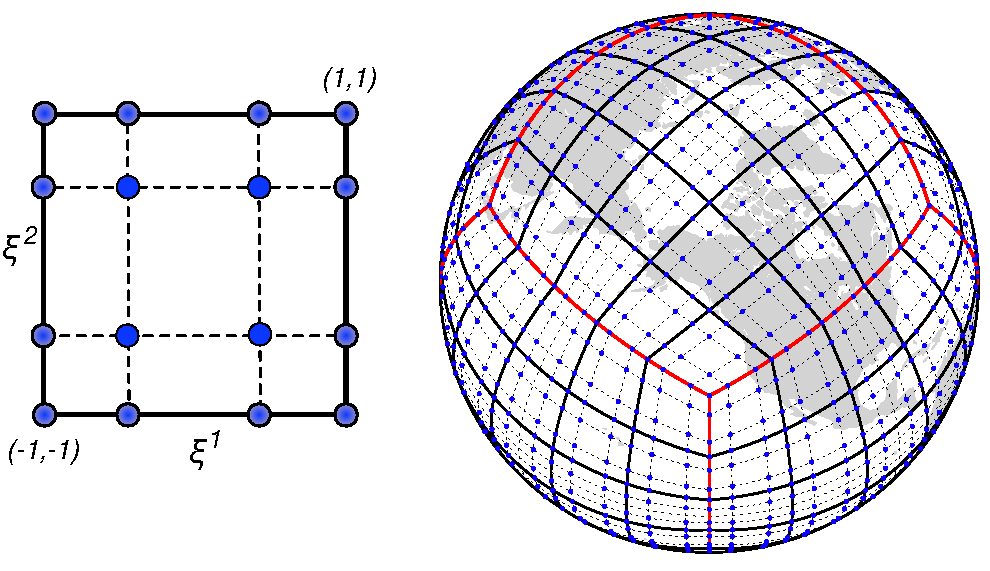
\includegraphics[scale=0.75]{figs/cs_gll4_2017}
 \caption{The left panel shows the  Gauss-Lobatto-Legendre (GLL)   grid with $ N_p \times  N_p$ quadrature points defined
 on a standard element $[-1,1]^2$, where $N_p=4$. The right panel shows the cubed-sphere ($\mathcal{S}$) grid system tiled with 
 $6 N_e^2 $ spectral elements $\Omega_e$, where $N_e$ is the number of elements  in each coordinate direction
 on a panel (in this case $N_e=5$). 
 Each element  $\Omega_e$ on $\mathcal{S}$ has the GLL grid structure.  }
 \label{fig:gll4}
\end{figure}
    The CAM-SE 
 uses a cubed-sphere geometry  originally introduced by \cite{S1972MWR}  to represent the planet earth. The  spherical   surface 
  $\mathcal{S}$ is  a patched domain,  which is partitioned  into   non-overlapping quadrilateral elements 
 $\Omega_e$ such that $\mathcal{S} = \cup \, \Omega_e$ (see Fig.~\ref{fig:gll4}). 
  On   $\mathcal{S}$  each 2D  element $\Omega_e(x^1,x^2)$  defined in terms of
 central  (gnomonic) projection angles $x^1,x^2 \in [-\pi/4, \pi/4]$, which serve as  the independent variables in the computational domain. 
 The mapping from cube to sphere results in a non-orthogonal curvilinear  coordinate system on $\mathcal{S}$, with 
 the  metric tensor $G_{ij}$ and  analytic Jacobian $ \sqrt{G} =  |G_{ij}|^{1/2}$, $i, j \in \{1,2\}$. 
 A  physical vector quantity  such as the wind vector $\mathbf{v} = (u,v)$,  defined on  $\mathcal{S}$
 in  orthogonal lat-lon coordinates,  can  be uniquely
 expressed in tensor form using conventional notations as the covariant $(u_1,u_2)$ and contravariant  $(u^1, u^2)$ vectors 
 using the  $2 \times 2$ transformation matrix  $\mathbf{D}$ associated with the gnomonic mapping 
 such that   $\mathbf{D}^T\mathbf{D} = G_{ij}$ (see \cite{NTL2005MWR} for the details):  
  %   
    \begin{equation}
     \left[   \begin{array}{c}
               u \\ v
             \end{array}
           \right]
           =
     \mathbf{D}  \, \left[   \begin{array}{c}
               u^1 \\ u^2
             \end{array}
           \right] =
            \mathbf{D}^{-T}  \, \left[   \begin{array}{c}
               u_1 \\ u_2
             \end{array}
           \right]. 
%          \quad \mathbf{D}^T\mathbf{D} = G_{ij}. 
          \label{eq:covcontra} 
\end{equation}

 The governing equations defined in familiar vector form can also be expressed 
 in  general tensor form. In order  to  describe the SE discretization process in simple terms, we consider the 
 the following conservation law  on $\mathcal{S}$ for an arbitrary  scalar $\phi$:  
 %
 \begin{equation}
 \frac{\partial \phi }{\partial t}  + \nabla \cdot \mathbf{F}(\phi)  = S(\phi),
 \label{eq:se1} 
 \end{equation}
where 
\begin{equation}
   \nabla \cdot \mathbf{F}(\phi) = \frac{1}{\sqrt{G}} \left[   \frac{\partial  \sqrt{G} F^1}{\partial x^1}  + 
   \frac{\partial  \sqrt{G} F^2}{\partial x^2}      \right] .  
   \end{equation} 
  %
In the special case of the flux-form transport equation the
   contravariant fluxes $(F^1, F^2) = (u^1 \phi , u^2 \phi)$, and $S(\phi)$  is an arbitrary source term.
%  and  the gradient $\nabla_h = (\partial/\partial x^1, \partial/\partial x^2)$ defined on computational domain $\mathcal{C}$ corresponding
%  to $\mathcal{S}$ under the gnomonic mapping.   Note that the flux-form  transport  equation  is a special case of (\ref{eq:se1}), with flux function
%  $(F^1, F^2) = (u^1 U,  u^2 U)$.


\subsection{\normalsize SE spatial discretization in 2D}

%In order to describe the spectral-element (SE) horizontal discretization as used in CAM-SE, we consider the
%following generic form  of a governing equation (33-35): 
% \begin{equation}
% \frac{\partial U }{\partial t}  + \nabla_h \cdot \mathbf{F}(U)  = S(U)   \quad   {\rm in} \quad \mathcal{S}, \label{eq:se1} 
% \end{equation} 
% %
%where $U$ is a prognostic variable defined on the spherical domain $\mathcal{S}$ and  $\nabla_h \cdot$ is the horizontal divergence operator. 
%$\mathbf{F}$ is a general  flux function and $S(U)$ is the source term, which can be
%a diffusive flux or any forcing term.  

The  SE solution process involves  casting the partial differential equation in Galerkin form, i.e.,  by multiplying  (\ref{eq:se1})  with a test (weight) function
$\psi$  and integrating over the domain $\mathcal{S}$, 
\begin{equation}
 \int_{\mathcal{S}} \psi \,  \left[ \frac{\partial \phi }{\partial t}  + \nabla \cdot \mathbf{F}(\phi) -  S(\phi)  \right]  d\mathcal{S}  = 0. \label{eq:se2} 
 \end{equation} 
A computational form of  (\ref{eq:se2})  is obtained by applying Green's theorem,  
resulting in  the weak Galerkin form, as follows: 
 %
 \begin{equation}
 \int_{\mathcal{S}} \psi   \ \frac{\partial \phi }{\partial t} \,   d\mathcal{S}  = 
  \int_{\mathcal{S}}  \nabla  \psi \cdot \mathbf{F}(\phi) \,  d\mathcal{S}  + 
       \int_{\mathcal{S}} \psi  \, S(\phi)  \,   d\mathcal{S}, \label{eq:se3} 
 \end{equation} 
 %
 where the approximation to the  solution $\phi$ and the test function belong to a polynomial space  $V^{N}$. 
 The SE method consists of  partitioning the domain into non-overlapping elements and solving the global problem 
 locally on each element, where the  solution is approximated by using a set of  basis (polynomial) functions of prescribed 
 order $N$.  A basic assumption used in SE (or continuous Galerkin) method is that the global basis 
 corresponding to (\ref{eq:se3}) is 
 $C^0$ continuous. 
Therefore  the problem (\ref{eq:se3}) can be solved locally for each 
 element $\Omega_e$, if there is a mechanism by which the solution maintains $C^0$ 
 continuity at the element boundaries as required 
 by the SE  discretization.   
 %
%
 
 For efficient evaluation of the integral equation (\ref{eq:se3}), the SE  method employs the Gauss-Lobatto-Legendre (GLL) 
  quadrature rule for integrals and collocation differentiation for derivative operators. All the corresponding numerical 
  operations are performed on a square   $[-1,1]^2$ known as  the standard  (or reference) element.   
%  For that each 2D  element $\Omega_e(x^1,x^2)$  defined in terms of
% central angles $x^1,x^2 \in [-\pi/4, \pi/4]$, which are  essentially the independent variables 
% in the physical domain (Nair et al. 2004).  
 In order to facilitate local mesh refinement,   
  the spectral elements  $\Omega_e$  on $\mathcal{S}$ are defined as arbitrary spherical quadrilaterals
  in  the CAM-SE  grid system, which should   be  mapped onto  the standard element.
  A direct  way to address this problem is establishing  % a composite mapping  in computational space. 
  a  transformation  $\mathcal{J}_e: \Omega_e \rightarrow [-1,1]^2$, where    $\mathcal{J}_e$
  may be considered as   a  composite mapping combining the gnomonic and  the quadrilateral to standard-element mapping.
  Let the Jacobian  associated  with the composite mapping be $J_e = J_e(\sqrt{G})$.
   Then   an  arbitrary surface integral  on $\Omega_e$ can be expressed in terms of local coordinates $\xi^1, \xi^2 \in [-1, 1] $
 and the Jacobian  $J_e$ 
   %
   \begin{equation}
 \int_{\Omega_e} \psi (x^1,x^2) \,  d\Omega_e =   \int_{-1}^{1} \int_{-1}^{1} J_e(\xi^1,\xi^2)  \,  \psi(\xi^1,\xi^2) \, d\xi^1 \, d\xi^2
   \approx   \sum_{k=0}^{N}   \sum_{l=0}^{N} w_k w_l \, J_e(\xi^1_k,\xi^2_l) \,   \psi(\xi^1_k,\xi^2_l),
                               \label{eq:se4} 
 \end{equation} 
 %
 where  $w_k, w_l$  are  the  Gauss  quadrature weights. 
 
 In the  case of GLL quadrature rule, the  nodal points $\xi_k$, $k=0, 1, \dots, N$, 
 are  the roots of  the polynomial $(1-\xi^2) P'_N(\xi) = 0$,
 $\xi \in [-1,1]$;   and the corresponding  GLL quadrature  weights are given by 
 \[   w_k =  \frac{2}{N(N+1) \, [P_N(\xi_k)]^2 },
 \] 
  where  $P_N(\xi)$ is the  Legendre polynomial of degree $N$. 

   For the SE discretization it is customary to use  Lagrange polynomials  $h_k(\xi)$,   with roots at  the 
 GLL   quadrature points $\xi_k$, as basis functions.  This setup provides  discrete orthogonality 
 for  the basis function $h_k(\xi)$,  which   is formally defined as: 
 %
 \begin{equation}
    h_k(\xi) = \frac{ (\xi^2-1)\, P'_N(\xi)}{ N (N+1)\, P_N(\xi_k) \,(\xi-\xi_k)}.   \label{eq:se5}
 \end{equation}
 %
  Note that there are $N+1 = N_p$ GLL quadrature points in 1D,
 and $N_p \times N_p$ GLL points are needed for 2D spectral elements $\Omega_e$. 
 Figure~(\ref{fig:gll4}) shows the GLL grid  with $N_p =4$ on the left panel, 
 and the right panel shows the cubed-sphere grid $\mathcal{S}$ tiled with elements $\Omega_e$,
 each with the GLL  grid points. 
 
  A semi-discrete  form of  (\ref{eq:se3})  on an  element $\Omega_e$ can by obtained by
   approximating the solution  as a tensor product of  1D Lagrange basis  $\{ h_k(\xi)\}_{k=0}^N$ such that
  %
 \begin{equation}
     \phi |_{\Omega_e} \approx  \phi^e(\xi^1,\xi^2,t) =  
              \sum_{k=0}^{N}   \sum_{l=0}^{N}  \phi^e_{kl}(t)  \, h_k(\xi^1) \, h_l(\xi^2),  \label{eq:se60}
 \end{equation}
 %
 where $\phi^e_{kl}(t) = \phi^e(\xi_k^1, \xi_l^2,t) $ are  the nodal grid-point values of the solution, and  defining the  test function as
  $\psi(\xi^1,\xi^2) = h_k(\xi^1) \, h_l(\xi^2)$.\\ 


 By using (\ref{eq:se4}) and the discrete orthogonality property of $h_k(\xi)$, 
  we get a completely decoupled system of ODEs on  $\Omega_e$,  for each grid-point $(k,l)$ 
  %
  \begin{eqnarray}
      \widetilde M^e_{kl}\, \, \frac{d }{dt} \phi^e_{kl}(t) &= &  A^e_{kl}    + S^e_{kl}  \label{eq:se6} \\
        \widetilde M^e_{kl}  &=  & \int_{-1}^{1} \int_{-1}^{1} J_e  \, h_k(\xi^1)  \, h_l(\xi^2) \, d\xi^1  d\xi^2 = J_e(k,l) \, w_k \, w_l \\
          A^e_{kl}  &=  & \sum_{i=0}^N  J^{(1)}_e(i,l) \,  F^1_{i l} \, D_{ik}^{(1)}\, w_i  w_l  +
           \sum_{i=0}^N  J^{(2)}_e(k, i) \,  F^2_{k i} \, D_{l i}^{(2)} \, w_k  w_i \\
           S^e_{kl}  &=   &J_e(k,l) \, w_k w_l  \, S(U_{kl})
  \end{eqnarray}  
  %
  %where $  \widetilde M^e_{kl}$ is the so-called  mass matrix, $(F^1,F^2) = \mathbf{F}$  are  the  flux terms, 
   where $J^{(i)}_e = J_e \,\partial \xi^i / \partial x^i$ is the metric term  and 
   $D^{(i)}_{lk}$ is the  derivative matrix $h'_k(\xi^i_l)$, 
  along the $x^i$-direction and  $ i \in \{1,  2\}$. 

 The ODEs  (\ref{eq:se6}) can be written in a formal matrix-vector form
  for  $\Omega_e$  following
  \cite{KS2013book}: 
  %
 \begin{equation}
    \widetilde{\mathbf{M}}^e\, \, \frac{d }{dt} \Phi^e =   \mathbf{A}^e    + \mathbf{S}^e + \mathbf{B}^e,  \label{eq:se7} 
 \end{equation}
      %
      where $\widetilde{\mathbf{M}}^e$ is the  so-called mass matrix,  which  is a diagonal  matrix with entries $\widetilde M^e_{kl}$.    $\mathbf{B}^e$
  indicates the boundary terms for the element 
  $\Omega_e$, which is a key component linking  the local and global problem (\ref{eq:se3}) and enforcing $C^0$ continuity
  for solutions across element boundaries.  
  
  The  global matrices associated with  (\ref{eq:se3}) can be obtained 
  by  summing the contributions from elemental matrices  and  this procedure is known as the 
  direct stiffness summation (DSS). However the global matrices are  not explicitly constructed. 
  In practice, the DSS operation replaces  interface values  of two  contiguous elements sharing the same physical location  
  by the  weighted sum (average)  so that  the boundary  nodes get unique values,   
   which maintains the continuity of the global solution across the element edges. This strategy has been adopted in CAM-SE. 
  Note that the DSS operation does not affect interior nodal values of any element, and  preserves global conservation of the SE discretization
  for (\ref{eq:se1}).  The elemental discretization (\ref{eq:se7}) combined with the  DSS operation  leads 
  to the time-dependent  system of ODE corresponding to (\ref{eq:se1}),
     \begin{equation}
  \frac{d }{dt} \phi(t) =   DSS(\phi).  \label{eq:se8}
       \end{equation}
The details of the discretization of the dissipation operators are provided in Appendix \ref{sec:dissipation}.

{\color{red}{Note that nodes on the element boundary are shared between elements and that after each Runge-Kutta step the shared nodes will have different values. The elements are coupled by averaging the two solutions at the shared nodes (so the halo communicated between elements is only one node/point deep). This is referred to as the DSS operation. The basis function representation of the solution is therefore only $C^0$ at element boundaries. The ability to obtain high-order accuracy with only edge point communication is an attractive feature of the spectral element method \citep{MadayPatera87,canuto2007}. Another aspect of the spectral element is that the basis function representation is spectral on each element so if, for example, one of the quadrature values are changed then it affects the basis functions throughout the element (except at the GLL nodes)}}.

%
\subsection{Mimetic discretization}
A numerical method is mimetic (or compatible) if key integral properties of divergence, gradient and curl-operators are mimicked in discretized space. The CAM-SE discretization satisfies the divergence/gradient adjoint relation
\begin{equation}
\int \phi \nabla \cdot \mathbf{v} \, d\mathcal{S}+\int \mathbf{v} \cdot \nabla \phi \, d\mathcal{S}=0
\end{equation}
in  discretized space \citep{TF2010JCP}. This property can be used to show the inherent conservation properties of CAM-SE {\color{red}{in the horizontal discretization \citep[see ][ for details]{T2011LNCSEb}. Mass is conserved and, in the absence of viscosity terms, energy is conserved with exact timestepping}}. 

Since the CAM-SE discretization is mimetic the adiabatic, frictionless discretization of the equations of motion conserves total moist energy to within time-truncation errors. The equivalent internal energy change due to hyperviscosity damping of the velocity vector is added as frictional heating in the thermodynamic equation so the energy budget for the viscosity on the momentum equations is closed. The dissipation of energy due to hyperviscosity on temperature and dry-mass, however, is not energy-conserving. The vertical remapping does not conserve total energy either but it does conserve moist internal energy and AAM. {\color{red}{Hyperviscosity reduces variance but is a mass-conserving operation in CAM-SE.}}


% CAM-SE is based on a continuous Galerkin finite-element (or spectral-element) method \citep{TTI1997JCP} and is discretized using a cubed-sphere tiling of the sphere. Petascale scalability of CAM-SE was demonstrated in \cite{DetAl2012IJHPCA}. Also, CAM-SE provided refined mesh functionality in CAM \cite[e.g., ][]{SJDTT2008MWR,ZetAl2014JC}, improved accuracy of idealized baroclinic wave simulation \citep{LJTN2010JAMES}, conserved total energy to time-truncation errors \citep{T2011LNCSEb} and improved global axial angular momentum budgets compared to CAM-FV \citep{LBDL2014JAMES}. That said, the tracer transport component of CAM-SE appeared to be less accurate than CAM-FV for non-smooth tracer distributions \citep{LetAl2011GMD,HetAl2016QJRMS}. In an idealized terminator test in which two species react according to a reaction coefficient proportional to the solar terminator while being transported by an idealized 2D flow, CAM-SE produces errors larger than CAM-FV \citep{LCLVT2015GMD}. The errors are due to the limiter used for tracer transport that prevents oscillatory (and in particular negative) solutions for tracers \citep{GTS2014JCP}. In terms of computational throughput it was also found that CAM-SE was slower for large tracer counts (at least when run with core counts similar to the non-scalable CAM-FV).

\subsection{Temporal discretization}
In a typical CAM setup where the model top is approximately 40km, the maximum stable time-step for solving the continuity equation for water species $\ell$, $\ell \in \mathcal{L}_{water}$ (referred to as tracer advection), is limited by the maximum horizontal advective wind speed. The maximum stable time-step for the remaining equations of motion (thermodynamic equation, momentum equations and the continuity equation for dry air) is limited by the fastest gravity waves.  Since the maximum advective winds are typically slower than the fastest gravity waves, different time-stepping methods are used for tracer advection and the remaining equations of motion. While the overall time-step is the same, different Runge-Kutta (RK) methods are used to maintain stability. 

The SE tracer advection algorithm uses a three-stage RK strong-stability-preserving (SSP) time-stepping method, ensuring the time step will preserve any shape-preserving properties preserved by the underlying spatial discretization \citep{SR2002SIAM}. The shape-preserving filter used is described in \citet{GTS2014JCP}. The shape-preserving SE tracer advection algorithm is formally second-order accurate.

The momentum, thermodynamic and dry air continuity equations are solved using an explicit nonlinearly third-order accurate five-stage Runga-Kutta method based on \cite{KG1984MCSb} and described in \cite[][ see their equation (56)]{GU2016GMD}. For sake of completeness, this scheme is described in appendix \ref{app:KG53}, and will be referred to as KG53.  The inviscid equations of motion are advanced one dynamics time-step using the KG53 method followed by an application of the hyperviscosity operators through solving the advection-diffusion equation of the updated prognostic variables using forward Euler time-stepping. Note that it is necessary to subcycle the hyperviscosity-step for stability. The viscosity terms are computed as described in section \ref{sec:hyper} and discretized using the SE method presented in Appendix \ref{sec:dissipation}.

%{\color{red}{[Mark: How is tracer advection coupled to dry air continuity equation??]}} 

The time-steps in CAM-SE are controlled with namelist variables {\tt{se\_nsplit}}, {\tt{se\_rsplit}}, {\tt{se\_qsplit}},
{\tt{se\_hypervis\_subcycle}}  so that the time-steps for vertical remapping $\Delta t_{remap}$, tracer advection $\Delta t_{trac}$ (RK3), KG53 time-stepping for non-tracers $\Delta t_{dyn}$, and hyperviscosity $\Delta t_{hyper}$ are
\begin{align}
\Delta t_{remap}&=\frac{\Delta t_{phys}}{\tt{se\_nsplit}},\\
\Delta t_{tracer}&=\frac{\Delta t_{phys}}{\tt{se\_nsplit}*\tt{se\_qsplit}},\\
\Delta t_{dyn}&=\frac{\Delta t_{phys}}{\tt{se\_nsplit*se\_rsplit}*\tt{se\_qsplit}},\\
\Delta t_{hyper}&=\frac{\Delta t_{phys}}{\tt{se\_nsplit*se\_rsplit*se\_hypervis\_subcycle}*\tt{se\_qsplit}},
\end{align}
where $\Delta t_{phys}$ is the time-step used for computing physics tendencies. For the $1^\circ$ configuration ($N_e=30$, $N_p=4$ where $N_e$ is the number of elements in each coordinate direction on a panel and $N_p$ is the number of quadrature points along each coordinate direction in an element) the physics time-step is $\Delta t_{phys}=30 min$, and the subcycling parameters are {\tt{se\_nsplit}=2}, {\tt{se\_rsplit=3}}, {\tt{se\_qsplit=1}} and {\tt{se\_hypervis\_subcycle=3}}. See Table \ref{table:subc} for other resolutions.

 \begin{table}
 \caption{The table shows physics time-step (column 3), sub-cycling parameters (columns 4-6) as a function of resolution (column 1-2). The horizontal resolution is specified in the format $ne30np4$ which refers to $N_e=30$ and $N_p=4$; similar for other resolutions.  $N_e=0$ denotes a variable-resolution configuration. The approximate average quadrature node spacing at the Equator, $\Delta x_{ave}$ (in kilometers), is also listed (column 2). For all configurations presented in this paper {\tt{se\_qsplit}}=1.}
 \centering
 \begin{tabular}{llcccc}
 \hline
 Horizontal res. & $\Delta x_{ave}$  & $\Delta t_{phys}$ & {\tt{se\_nsplit}} & {\tt{se\_rsplit}} & {\tt{se\_hypervis\_}} \\
 &&&&&{\tt subcycle} \\
 \hline
   {\tt{ne}}16{\tt{np4}}  & $\sim$208km   & 1800s & 1 & 3 & 3  \\
   {\tt{ne}}30{\tt{np4}}  & $\sim$111km   & 1800s & 2 & 3 & 3  \\
   {\tt{ne}}60{\tt{np4}}  & $\sim$ 56km   & 900s  & 2 & 3 & 3  \\
   {\tt{ne}}120{\tt{np4}} & $\sim$28km    & 450s  & 2 & 3 & 3  \\
   {\tt{ne}}240{\tt{np4}} &  $\sim$14km   & 225s  & 2 & 3 & 3  \\
   {\tt{ne}}0{\tt{np4CONUS30x8}}  & $\sim$111km$\rightarrow$ $\sim$14km &  600s & 5 & 3 & 4  \\
 \hline
% \multicolumn{2}{l}{$^{a}$Footnote text here.}
 \end{tabular}
 \label{table:subc}
 \end{table}

%
\subsection{Coupling to physics}
CAM-SE uses a time-split approach in which dynamics advances the model state and the physics tendencies are based on the dynamics updated state. When CAM-SE starts a simulation, the physics are called first and then the  dynamics. The question is then how to add the physics tendencies in the dynamical core. CAM-SE supports several physics-dynamics coupling methods. Let $F_X$ be the physics tendency for prognostic variable $X$ in level $k$ (for notational simplicity the vertical index is dropped). The different coupling methods are detailed below and are identified with the rather arbitrary name `ftype'. A fuller discussion with results about different coupling methods is the content of a separate paper. Some results are provided by \citet{TJ2016GMD}.
\subsubsection{`ftype=0' configuration (default)}
In this case, compute the physics tendencies and add $\Delta t_{remap}F_X$ to the state of $X$, advance the dynamics $\Delta t_{remap}$ seconds based on the updated state, add $\Delta t_{remap}F_X$ to the dynamics updated state of $X$ and advance the dynamical core, and so on. In other words, the forcing is split into $\frac{\Delta t_{phys}}{\Delta_{remap}}$ equal chunks and added throughout the dynamics. The `ftype=0'-option is used by default in CAM-SE and used for all simulations presented in this paper.

The CAM parameterization package returns mixing ratio tendencies for tracers. We convert the mixing ratio tendencies to mass tendencies $F_X \Delta M^{(d)}_k$ since the prognostic variable for tracers in the dynamical core is $\Delta M_k m^{(d)}_k$.

Generally modelers do not allow the tracer tendencies to drive the mixing ratio of tracers negative, however, this may happen using `ftype=0'. If the tendency drives a mixing ratio negative, the mixing ratio is set to zero. In this case, only a fraction of the entire tracer tendency is added, leading to an inconsistency in how much mass the physics package wants to remove and the amount of tracer mass actually removed in the physics-dynamics coupling code in the dynamical core.
\subsubsection{`ftype=1' configuration}
In this configuration the entire physics forcing is added to the
dynamics state $\Delta t_{phys}F_X$ which is equivalent to having the
physics module update the model state. This coupling method is used in
CAM-FV \citep{L2004MWR}. Note that contrary to the `ftype=0'
configuration, this configuration always provides a closed mass budget
for tracers in terms of physics tendencies being fully applied in the
dynamical core. The disadvantage of using 'ftype=1' in CAM-SE is that
the use of a long physics time-step results in the appearance of
spurious gravity waves due to large physics tendencies.
\subsubsection{`ftype=2' configuration}
This configuration constitutes a hybrid approach where mass variables (tracers) use the `ftype=1' physics-dynamics coupling method and all other variables use the `ftype=0' method.


%%%%%%%%%%%%%%%%%%%%%%%%%%%%%%%%%%%%%%%%%%%%%%%%%%%%%%%%%%%%%%%%%%%%%%%%%%%%%%%%%%%%%%%%%%%%%%%%%%%%%%%%%%%%%%%%%%%%%%%%%%%%%%
%%%%%%%%%%%%%%%%%%%%%%%%%%%%%%%%%%%%%%%%%%%%%%%%%%%%%%%%%%%%%%%%%%%%%%%%%%%%%%%%%%%%%%%%%%%%%%%%%%%%%%%%%%%%%%%%%%%%%%%%
\section{Results}\label{sec:results}
The evaluation of the SE dynamical core with CAM6 physics in an AMIP configuration simulation is the subject of a separate paper. Here the new dynamical core is evaluated in simpler configurations. First the new dynamical core version is compared with the old version using an idealized moist baroclinic wave thereby avoiding the complexity of a full physics parameterization suite that may make it harder to distinguish between cause and effect. It is confirmed that the new SE dynamical core version converges to within the uncertainty of high resolution reference solutions computed with the old SE dynamical core (that has been extensively validated) and the current `workhorse' dynamical core for $1^\circ$ climate simulation; CAM-FV \citep[finite-volume][]{L2004MWR}. Second, the dynamical core is evaluated in an aqua-planet setup \citep{NH2000ASL,WetAl2012NCAR,MWO2016JAMES} using CAM6 physics. In this context the conservation properties AAM and total moist energy is discussed. Thirdly the computational efficiency of CAM-SE is evaluated.
\subsection{Idealized moist baroclinic wave with Kessler microphysics}
For the validation of the new dynamical core version in a simplified setup, we use a moist variant of the dry baroclinic wave of \citet{UMJS2014QJRMS} with Kessler microphysics \citep{K1969MM}. This test case configuration was part of the Dynamical Core Model Intercomparison Project (DCMIP) 2016 test case suite \citep[][]{DCMIP16}. The initialization of the atmospheric state for the moist baroclinic wave is based on analytic expressions for $T_v$, $\mathbf{v}$, p and $q^{(wv)}$ as a function of latitude and height; $(\varphi,z)$. The surface geopotential is constant, $\Phi_s=0$, and the moist surface pressure is constant $p_s=1000hPa$. The analytical expressions for temperature, velocity components, (moist) pressure and specific humidity, denoted ${T_v}(\varphi,z)$, ${\mathbf{v}}(\varphi,z)$, ${p}(\varphi,z)$, and $q^{(wv)}(\varphi,z)$, respectively, are given in Appendix \ref{app:analytic}. When using a moist vertical hybrid-pressure coordinate, the full level pressures $p_k$ of the initial condition are known from the hybrid coefficients, $A_k$ and $B_k$, and one can iteratively solve for $z_k$ given (moist) pressure: $p_k={p}(\varphi,z_k)$ \citep[see, ][]{UMJS2014QJRMS}. Once the full level heights, $z_k(\varphi)$, are known then the specific humidity, virtual temperature and velocity components can be computed by evaluating the analytical expressions at $(\varphi,z_k)$. In the DCMIP 2016 test case documentation the virtual temperature is converted to temperature using $T_v=T\left( 1+\epsilon q^{(wv)}\right)$. For a dry-mass vertical coordinate model the initialization procedure is more complicated as described below.

\subsubsection{Initialization of the moist baroclinic wave using a dry-mass vertical coordinate}
The challenge is to extract dry-mass from the initial state defined in terms of (moist) pressure and preserve a balanced initial condition. Since the initial condition does not contain condensates we can assume that moist air is a gas which will simplify the derivations. First we write the dry atmosphere hydrostatic relation \eqref{eq:dry_atm_hydro} in terms of specific humidity, virtual temperature and (moist) pressure
\begin{eqnarray}
\frac{\partial M^{(d)}}{\partial z}&=&-\rho^{(d)}\, ,\\
&=&-\frac{\rho}{1+m^{(wv)}},\\
&=&-\frac{p}{R^{(d)}T_v}\frac{1}{\left( 1+m^{(wv)}\right)},\\
&=&-\frac{p}{R^{(d)}T_v}\left(1-q^{(wv)}\right),
\end{eqnarray}
where we have substituted the ideal gas law and used $\left( \frac{1}{1+m^{(wv)}} \right)=\left( 1-q^{(wv)} \right)$ for an atmosphere not containing any condensates. Hence the dry-mass as a function of latitude, $\varphi$, and height, $z$, is
\begin{equation}
{M}^{(d)}(\varphi,z)=M^{(d)}_t-\int_z^{z_t}\frac{p(\varphi,z)}{R^{(d)} T_v(\varphi,z)}\left(1-q^{(wv)}(\varphi,z)\right) dz,\label{eq:Upd}
\end{equation}
where $z_t$ is the height of the model top computed by iteratively solving \eqref{eq:baroPmoist} with $p(\varphi,z)=p_t=g\, M^{(d)}_t$ (assuming there is no moisture above the model top). To initialize the dry mass levels $M^{(d)}_s$ is needed. It is computed by integrating \eqref{eq:Upd} with lower integral bound $z=z_s=0\, m$ and approximating the integral using 20 point Gaussian quadrature (high-order quadrature is necessary to reduce integral errors). The weight of dry air per unit area is shown on Figure \ref{fig:baro_init}. The full dry-mass levels are given in terms of the hybrid coefficients ${M_k^{(d)}}(\varphi)=A_k M^{(d)}_t+B_k {M_s^{(d)}}(\varphi)$. The height, $z_{k}(\varphi)$, of the full dry-mass levels are computed by iteratively solving \eqref{eq:Upd} with ${M}^{(d)}(\varphi,z_k)={M}_{k}^{(d)}(\varphi)$. Once the heights are known the virtual temperature and velocity components can be computed by evaluating the analytical expressions at $(\varphi,z_k)$ as is done for the moist vertical coordinate initialization. If we do the same for specific humidity then the moist surface pressure (which is a diagnostic when using dry-mass vertical coordinates) deviates more than 1 Pa in the tropics from the analytical value of 1000hPa  (see Figure \ref{fig:baro_init}). As a result a spurious zonal signal in surface pressure with the same amplitude as the initial gravity waves appears in the simulations. Hence specific humidity must be initialized more carefully in order to obtain a more balanced initial condition which is discussed in the next paragraph. 

As for $M^{(d)}$, the mass of water vapor $M^{(wv)}$ per unit area can be written as
\begin{equation}
{M}^{(wv)}(\varphi,z)=-\int_z^{z_t}\frac{p(\varphi,z)}{R^{(d)} T_v(\varphi,z)}q^{(wv)}(\varphi,z)\, dz,\label{eq:Upvw}
\end{equation}
so that the (moist) pressure at half levels can be computed as the sum of the weight of dry air and moisture per unit area  since there are no condensates present in the initial condition
\begin{equation}
p(\varphi,z_{k+1/2})=g\, {M}^{(d)}(\varphi,z_{k+1/2})+g\, {M}^{(wv)}(\varphi,z_{k+1/2}),
\end{equation}
where $z_{k+1/2}$ is computed by the same iterative procedure as for full levels. An integrated value for water vapor in a layer can now be computed from
\begin{equation}
m^{(wv)}(\varphi,z_k)=\frac{p(\varphi,z_{k+1/2})-p(\varphi,z_{k-1/2})}{g{M}^{(d)}(\varphi,z_{k+1/2})-g{M}^{(d)}(\varphi,z_{k-1/2})}-1.
\end{equation}
Using this method for initializing the mixing ratio for water vapor the moist surface pressure is within 0.01 Pa of the analytical value of $10^5$ Pa (see Figure \ref{fig:baro_init}). Once $m^{(wv)}(\varphi,z_k)$ is computed, the temperature $T(\varphi,z_k)$ can recovered from $T_v(\varphi,z_k)$ by using \eqref{eq:tv}.

\begin{figure}[h]
\centering
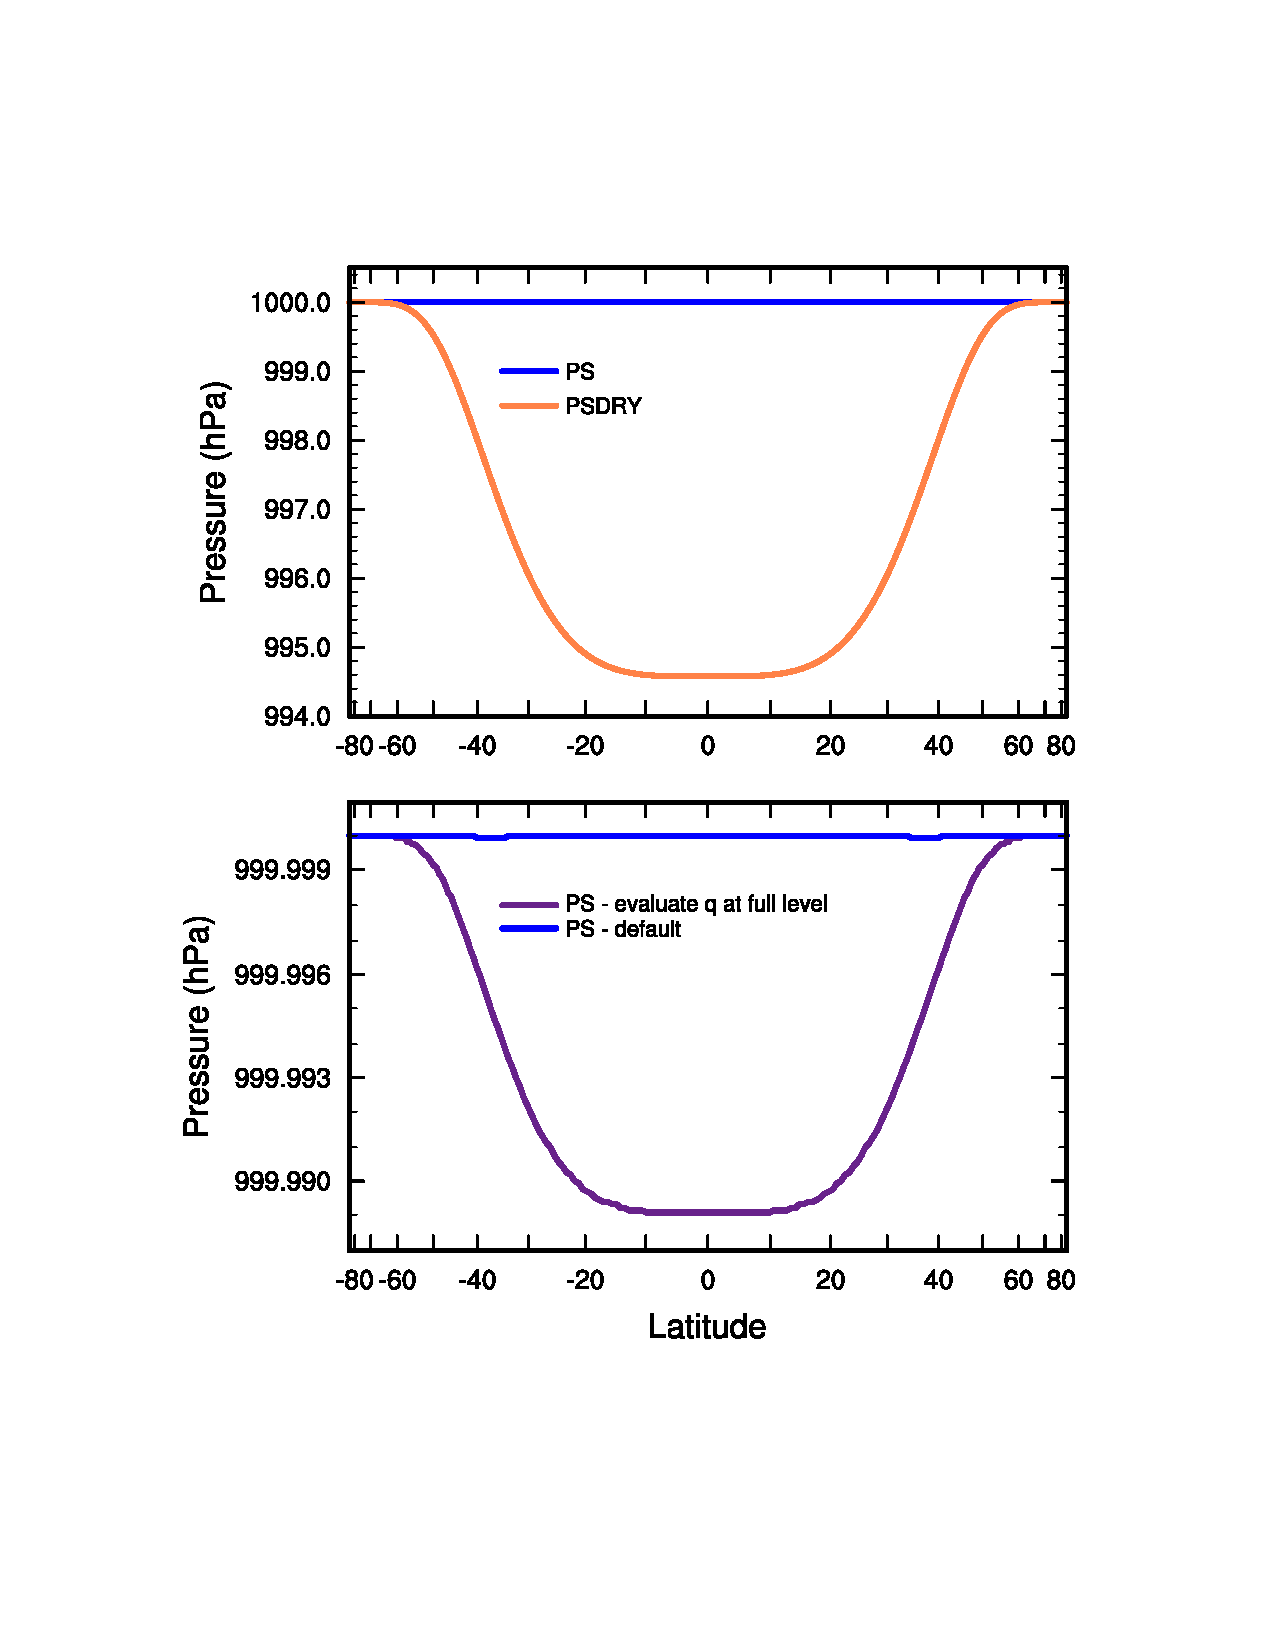
\includegraphics[width=20pc]{figs/01_baro_init.pdf}
\caption{(Upper) Zonally averaged weight of dry air per unit area (orange) and moist (blue) surface pressure as a function of latitude for the numerically computed initial condition for the moist baroclinic wave. Due to increased water vapor towards the Equator the dry mass decreases whereas the moist surface pressure is constant. (lower) Same as the upper plot but showing moist surface pressure where water vapor has been initialized by evaluating the analytic specific humidity formula at full levels (purple) and initializing the mixing ratio for water vapor in terms of moist and dry mass coordinates at half levels which effectively integrates humidity over the layer (blue). The lower plot uses 30 levels (CAM5). Note that the upper and lower plots have different scales on the $y$-axis.}
\label{fig:baro_init}
\end{figure}

%a shows the dry surface pressure as a function of latitude numerically computed with \eqref{eq:Upd}. From this surface pressure the dry pressure at model levels are computed from \eqref{eq:ABs}. We then iteratively solve \eqref{eq:Upd} to find the height $z_k$ of the full levels and this $z_k$ is then used to initialize temperature, wind and water vapor mixing ratio using the analytic expressions given in Appendix \ref{app:analytic}. The moist surface pressure can then be computed with \eqref{eq:halfpfull}. As shown in Figure \ref{fig:baro_init}(b) the diagnostic moist surface pressure is less than a Pascal of the analytic moist surface pressure of 1000hPa and the zonal structure in moist surface pressure has a much smaller amplitude than the gravity waves initially propagating from the wind perturbation.

\subsubsection{Simulation results}
As part of the `CESM simpler models' effort started by \citet{CESM_SIMPLER_MODELS}, the moist baroclinic wave setup has been implemented rigorously in the CESM in the sense that the configuration easily runs from CESM without code configurations using the `{\bf FKESSLER} compset'. For instructions on how to run the moist baroclinic wave with Kessler microphysics see \citet{FKESSLER}. Since the test case configuration has been implemented in the full CESM, the dynamical core interacts with the physics module as in full climate model simulations. Hence the global energy fixer is invoked \citep{WOHTTV2015JAMES} and for the dynamical cores using a (moist) pressure vertical coordinate there is an adjustment of specific humidity to conserve water after the moist physics updates \citep[see Section 3.1.6 in ][]{CAM5}. The intent of this implementation is to evaluate the dynamical core in simplified setup but exactly as the dynamical core is configured for comprehensive climate simulations.

Figure \ref{fig:baro_wave} depicts day 10 of the moist baroclinic wave test using the CAM-FV \citep[Finite-Volume; ][]{L2004MWR} dynamical core, CAM-HOMME dynamical core based on a moist vertical coordinate and the new dynamical core version (CAM-SE). The CAM-HOMME and CAM-SE (CESM2.0-SE) dynamical cores not only differ in terms of vertical coordinates but also in terms of hyperviscosity and the formula used for the heat-capacity in the thermodynamic equation. CAM-HOMME uses $c_p^{(d)}$ whereas CAM-SE (CESM2.0-SE) uses the comprehensive formula \eqref{eq:cp} that includes the heat capacity of water vapor.

\begin{figure}[h]
\centering
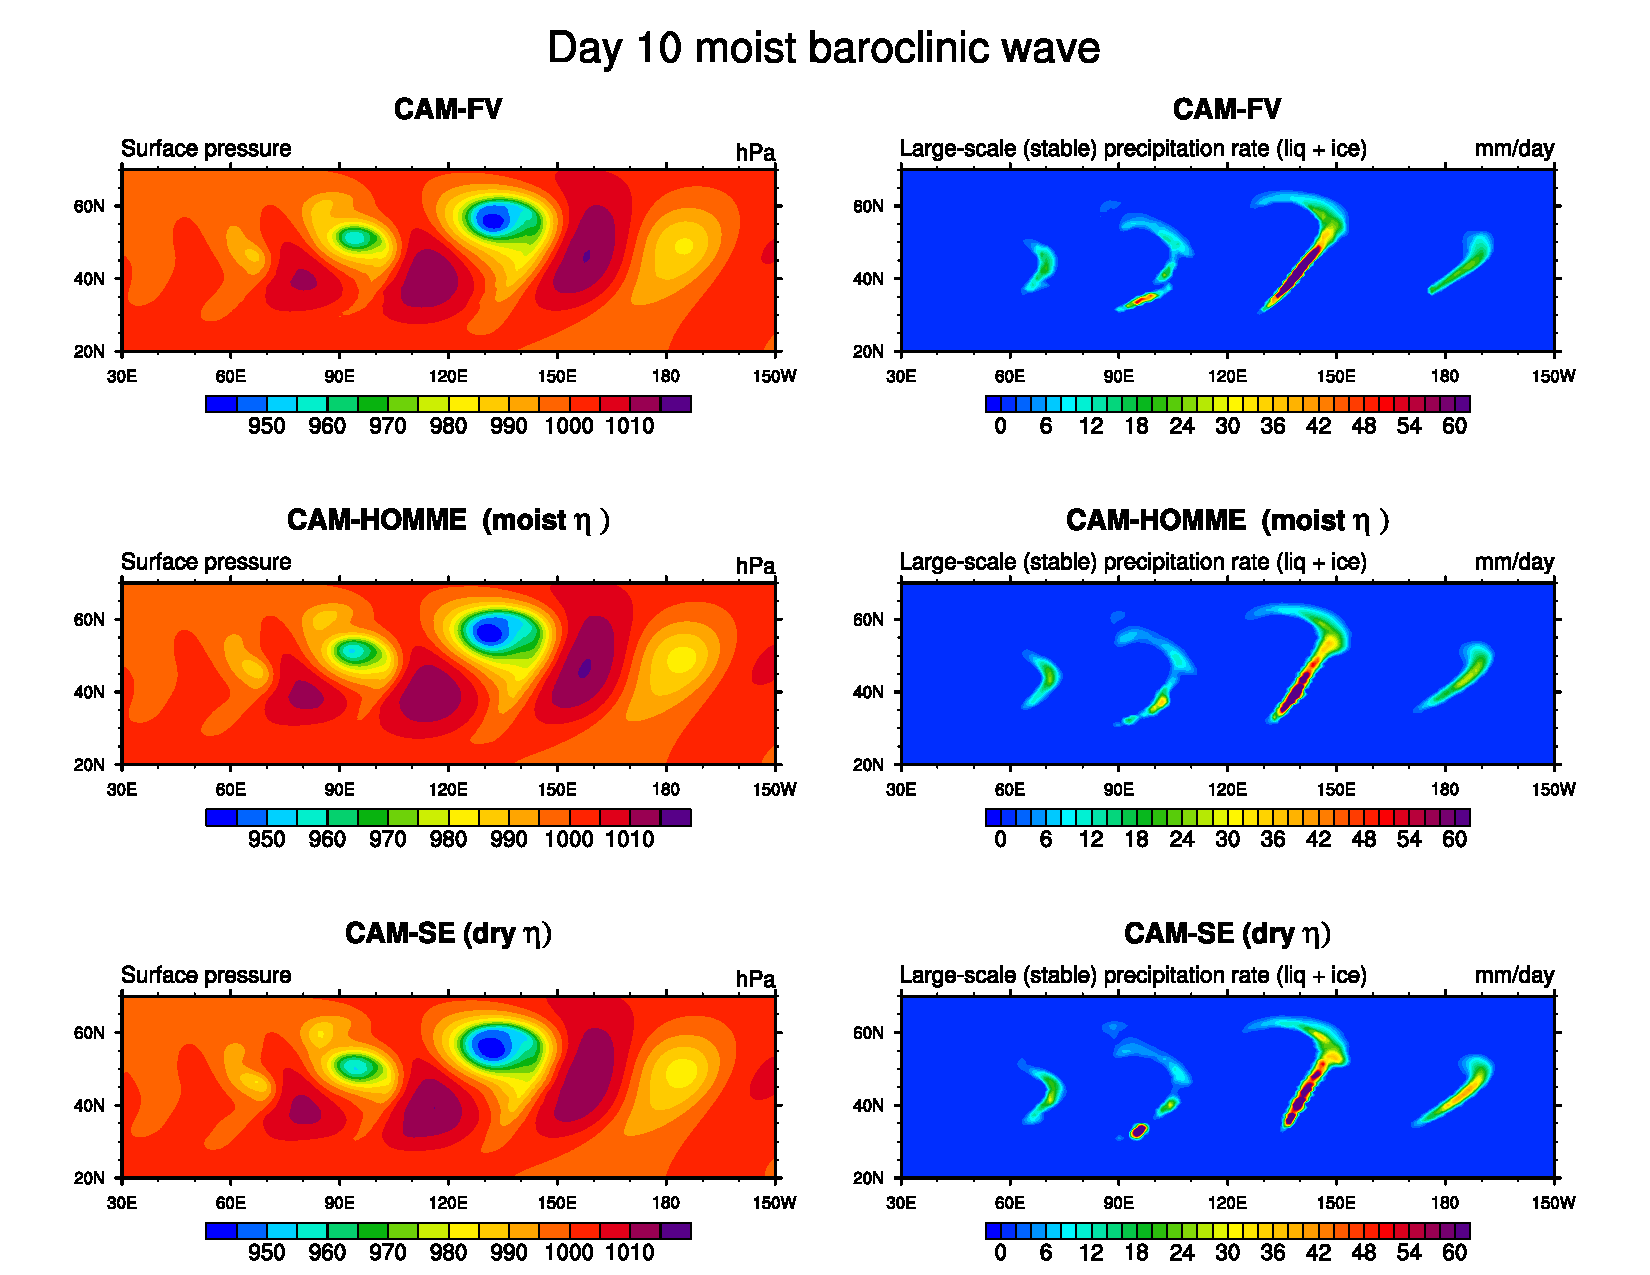
\includegraphics[width=33pc]{figs/02_baro_wave.pdf}
\caption{Left column shows moist surface pressure at day 10 for the moist baroclinic wave test case for (row 1) the finite-volume dynamical core, (row 2) CAM-HOMME version of the SE dynamical core based on a (moist) pressure vertical coordinate and (row 3) the dry-mass vertical coordinate version of SE presented in this paper. The right column is the same as the left but for large-scale precipitation rate. All results on this Figure are at $~1^\circ$ horizontal resolution.}
\label{fig:baro_wave}
\end{figure}

To provide a more quantitative measure of the difference between the moist baroclinic wave simulations, the $l_2$ difference norm of $p_s$ between two simulations is computed as the time varying global integral in spherical coordinates:

\begin{equation}
l_2\left(\,p_s(t)\,\right) = \left[ \frac{1}{4\pi}\int^{2\pi}_{0} \int^{\frac{\pi}{2}}_{-\frac{\pi}{2}} \ \left(\,p_{s_1}(\lambda,\varphi,t) - p_{s_0}(\lambda,\varphi,t)\,\right)^2 \, \cos(\varphi) \, d\varphi \, d\lambda \right]^\frac{1}{2}.
\end{equation}

The $l_2$ difference norm between CAM-SE and CAM-HOMME is shown in Figure \ref{fig:l2norm} for the $1^{\circ}$ ($N_e=30$ and $N_p=4$) and $\frac{1}{4}^{\circ}$ ($N_e=120$ and $N_p=4$) resolution simulations with 30 vertical levels (CAM5 level locations). The $l_2$ norms for the $1^{\circ}$ and $\frac{1}{4}^{\circ}$ simulations have similar time varying magnitudes. As the baroclinic waves evolves, the $l_2$ norms grow to a maximum on the order of 1 hPa by day 15. To assess the significance of the $l_2$ norms, an $l_2$ norm that serves as an estimate of the uncertainty of a high resolution reference simulation is computed following \cite{JW2006QJR}. The uncertainty in the reference is taken as the $l_2$ between a pair of $\frac{1}{4}^{\circ}$ resolution moist baroclinic wave simulations using different dynamical cores, CAM-SE and CAM-FV. At a $\frac{1}{4}^{\circ}$ resolution, the moist baroclinic wave solutions are converged to within a tolerable level of error (not shown), and therefore comparison between dynamical cores serves as an estimate of the uncertainty in the reference solutions arising from model imperfections. 

The black curve in Figure \ref{fig:l2norm} is the $l_2$ difference norm between CAM-SE and CAM-FV at approximately a $\frac{1}{4}^{\circ}$ resolution. $l_2$ values that fall below the uncertainty in the reference are considered insignificant. The $l_2$ between CAM-SE and CAM-HOMME generally lie near or below the uncertainty in the reference solution, indicating the differences between CAM-SE and CAM-HOMME are insignificant for the case of the moist baroclinic wave. This is consistent with the corresponding time varying, global minimum in $p_s$ for all the simulations, which illustrates that the differences between CAM-SE and CAM-HOMME are smaller than the differences arising from increasing the horizontal resolution.

\begin{figure}[h]
\centering
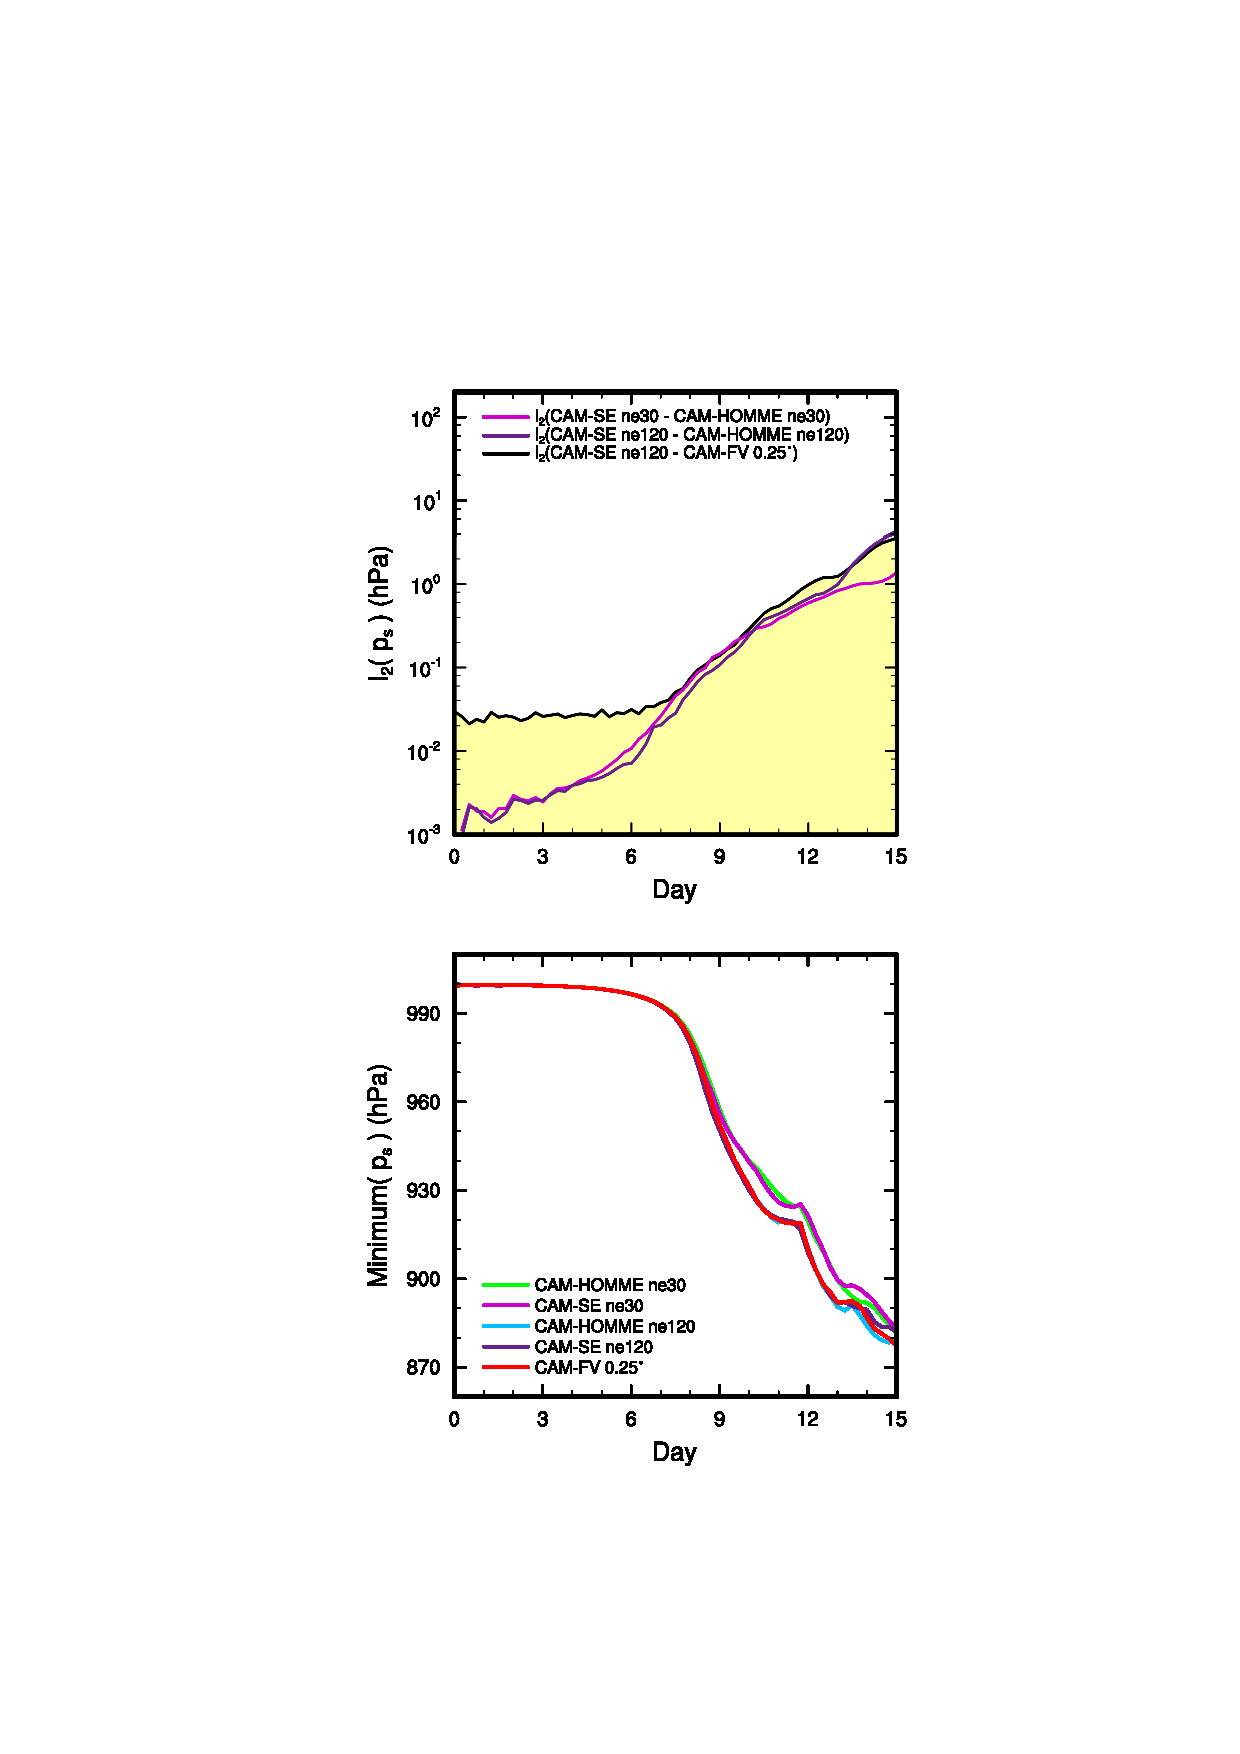
\includegraphics[width=20pc]{figs/l2.pdf}
\caption{(Upper) $l_2$ difference norms of $p_s$ in the moist baroclinic wave simulations. $l_2$ values lying within the yellow region fall below the estimate of the uncertainty in the reference solution (black curve). (lower) Global minimum $p_s$ in the moist baroclinic wave simulations.}
\label{fig:l2norm}
\end{figure}

\subsection{CAM6 aqua-planet simulations}\label{sec:APE}
The `CESM simpler models' effort also supports aqua-planet configurations \citep{MWO2016JAMES}. The aqua-planet configurations \citep{NH2000ASL} refer to an ocean covered planet with no axial tilt -- a planet in a perpetual equinox and devoid of continents. The aqua-planet compsets designate a fixed, zonally-symmetric SST distribution, modeled after the present day SST distribution on Earth (`QOBS' in \cite{NH2000ASL}). The lack of a seasonal cycle allows one to compute robust statistics from a shorter simulation, and the absence of land removes any influence of discretized topography or interactions with the land model from the simulations. The aqua-planet configurations are therefore an indispensable tool for testing design choices in global atmospheric models.

To understand how the design choices adopted by CAM-SE influence the aqua-planet solutions compared to its predecessor, CAM-HOMME, we ran a pair of simulations using the CAM6 physics package for 4.5 years at $~1^\circ$ horizontal resolution ($N_e=30$ and $N_p=4$) and 32 levels in the vertical {\color{red}{(model top is at approximately 3.6Pa)}}. Figure~\ref{fig:kespectra} shows the total kinetic energy spectrum at the 200 hPa level in the two simulations. Compared to CAM-HOMME, the slope of the kinetic energy spectrum in CAM-SE is shallower for wavenumbers larger than 30, bringing the solutions closer to the empirically \citep{NG1985JAS} and theoretically \citep{C1971JAS} determined slope of -3 at synoptic scales. {\color{red}{The increased kinetic energy at smaller scales is due to reducing the explicit diffusion coefficients used in CAM-SE compared to CAM-HOMME rather than the reformulation of the dynamical core in dry-mass vertical coordinates or a more comprehensive treatment of moist energy. Reducing the viscosity coefficients without increasing noise in the solutions (especially in the presence of `real-world' topography) has been made possible by damping momentum and temperature on approximate pressure levels and only damping the deviation of pressure-level thickness from a smoother reference pressure-level thickness.}}

%The increased kinetic energy at smaller scales is primarily the result of committing to smaller viscosity coefficients in CAM-SE (not shown).

\begin{figure}[h]
\centering
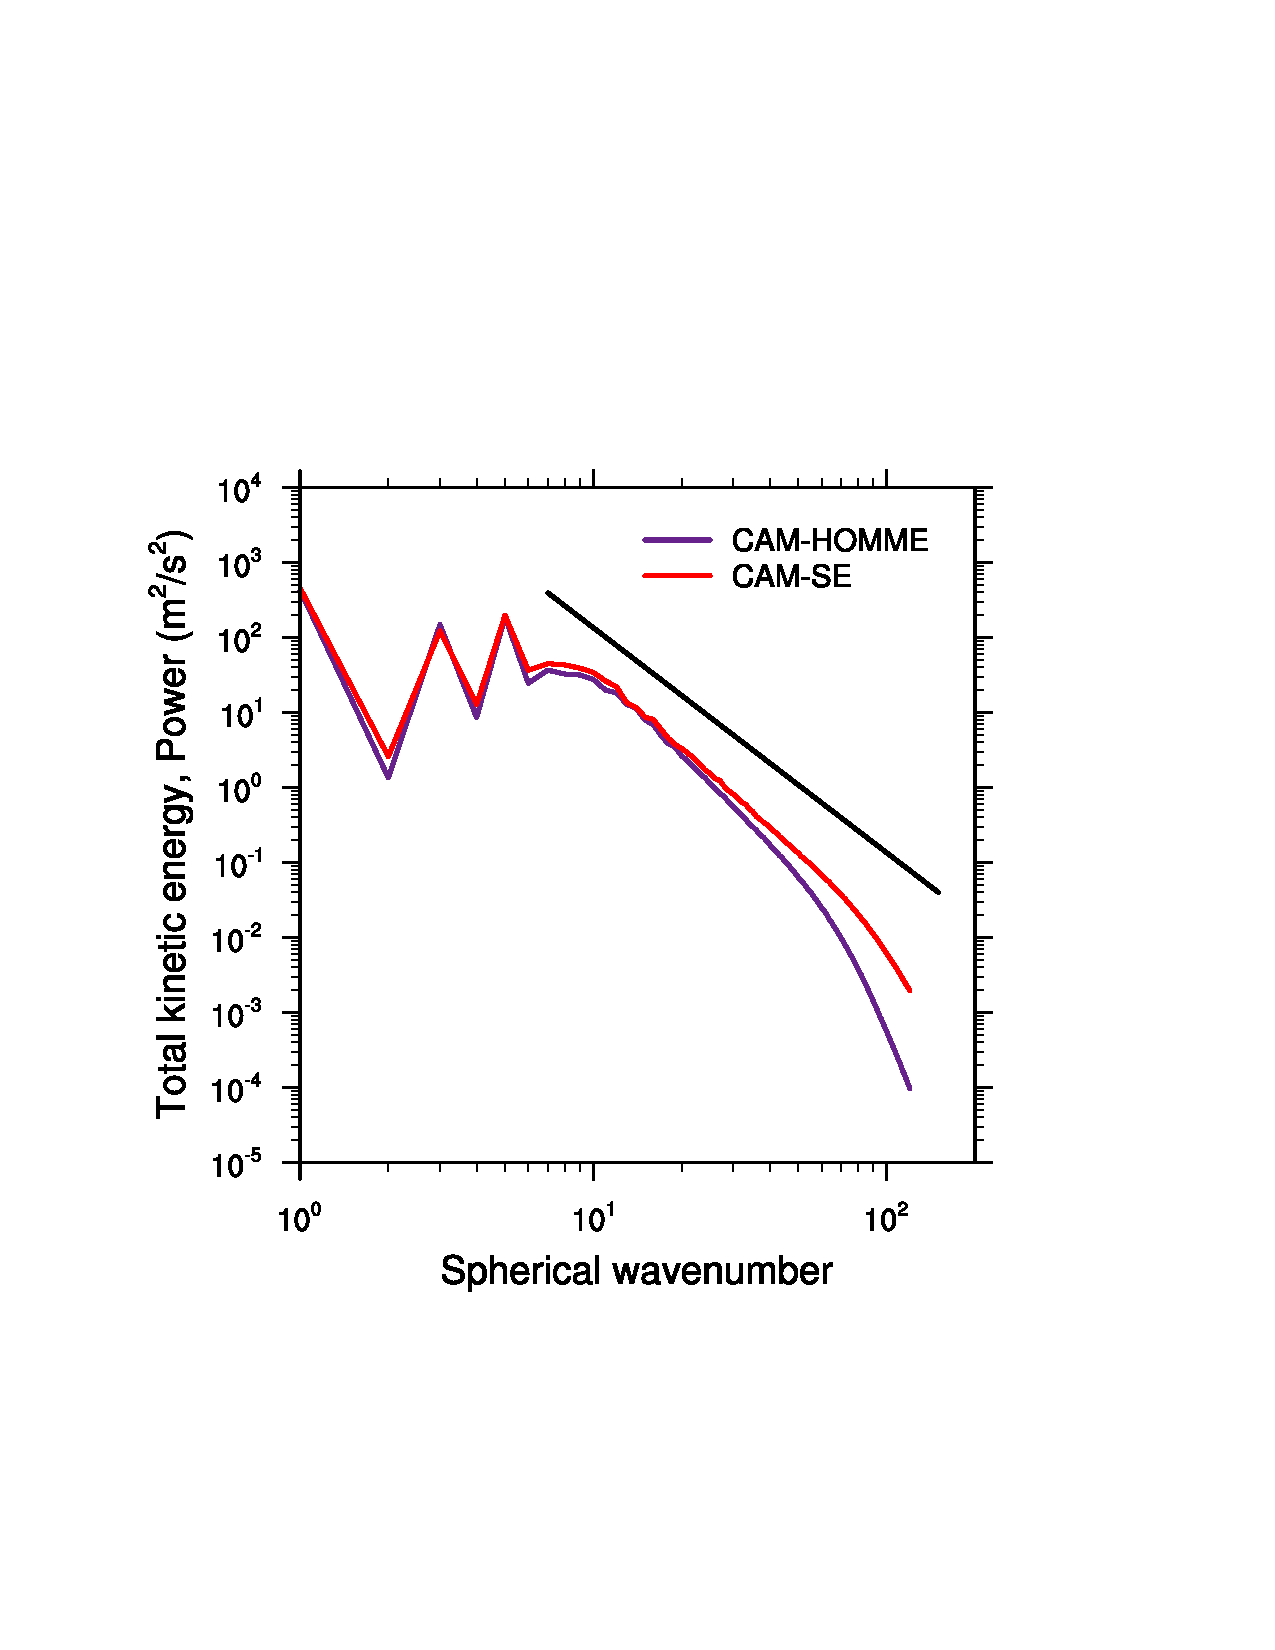
\includegraphics[width=20pc]{figs/kespectra.pdf}
\caption{Total kinetic energy spectrum of the horizontal winds at the 200 hPa level in CAM-HOMME and CAM-SE at $~1^\circ$ horizontal resolution ($N_e=30$ and $N_p=4$), computed as the mean spectra from 30 days of 6-hourly instantaneous spectra. Black line is the ${\kappa}^{-3}$ reference scaling, where $\kappa$ is wave-number.}
\label{fig:kespectra}
\end{figure}

Figure~\ref{fig:dzonal}a shows the zonally averaged total precipitation rate in CAM-HOMME (purple) and CAM-SE (red) averaged over the final 4 years of the simulations. The differences between the two simulations is provided as the purple curve of Figure~\ref{fig:dzonal}b. CAM-SE has increased precipitation at the equator, with a peak difference of 3 mm/day. An approximate 1 mm/day reduction in precipitation occurs on the flanks of the equator (Figure~\ref{fig:dzonal}). CAM-HOMME has twin Inter-Tropical Convergence Zones (ITCZ) straddling the equator, which is a common feature of the tropics in general circulation models (GCMs; \cite{BGN2010JCLIM}; \cite{MWO2016JAMES}), but appears absent from the CAM-SE simulations (Figure~\ref{fig:dzonal}). The total precipitation rate in the model is the sum of the precipitation from the convective parameterizations, and that due to large-scale condensation. The deep convective precipitation rate indicates that the double-ITCZ does exist in CAM-SE (not shown), but is masked by the large increase in total precipitation rate at the equator (Figure~\ref{fig:dzonal}b) primarily due to an increase in large-scale condensation (not shown).

\begin{figure}[h]
\centering
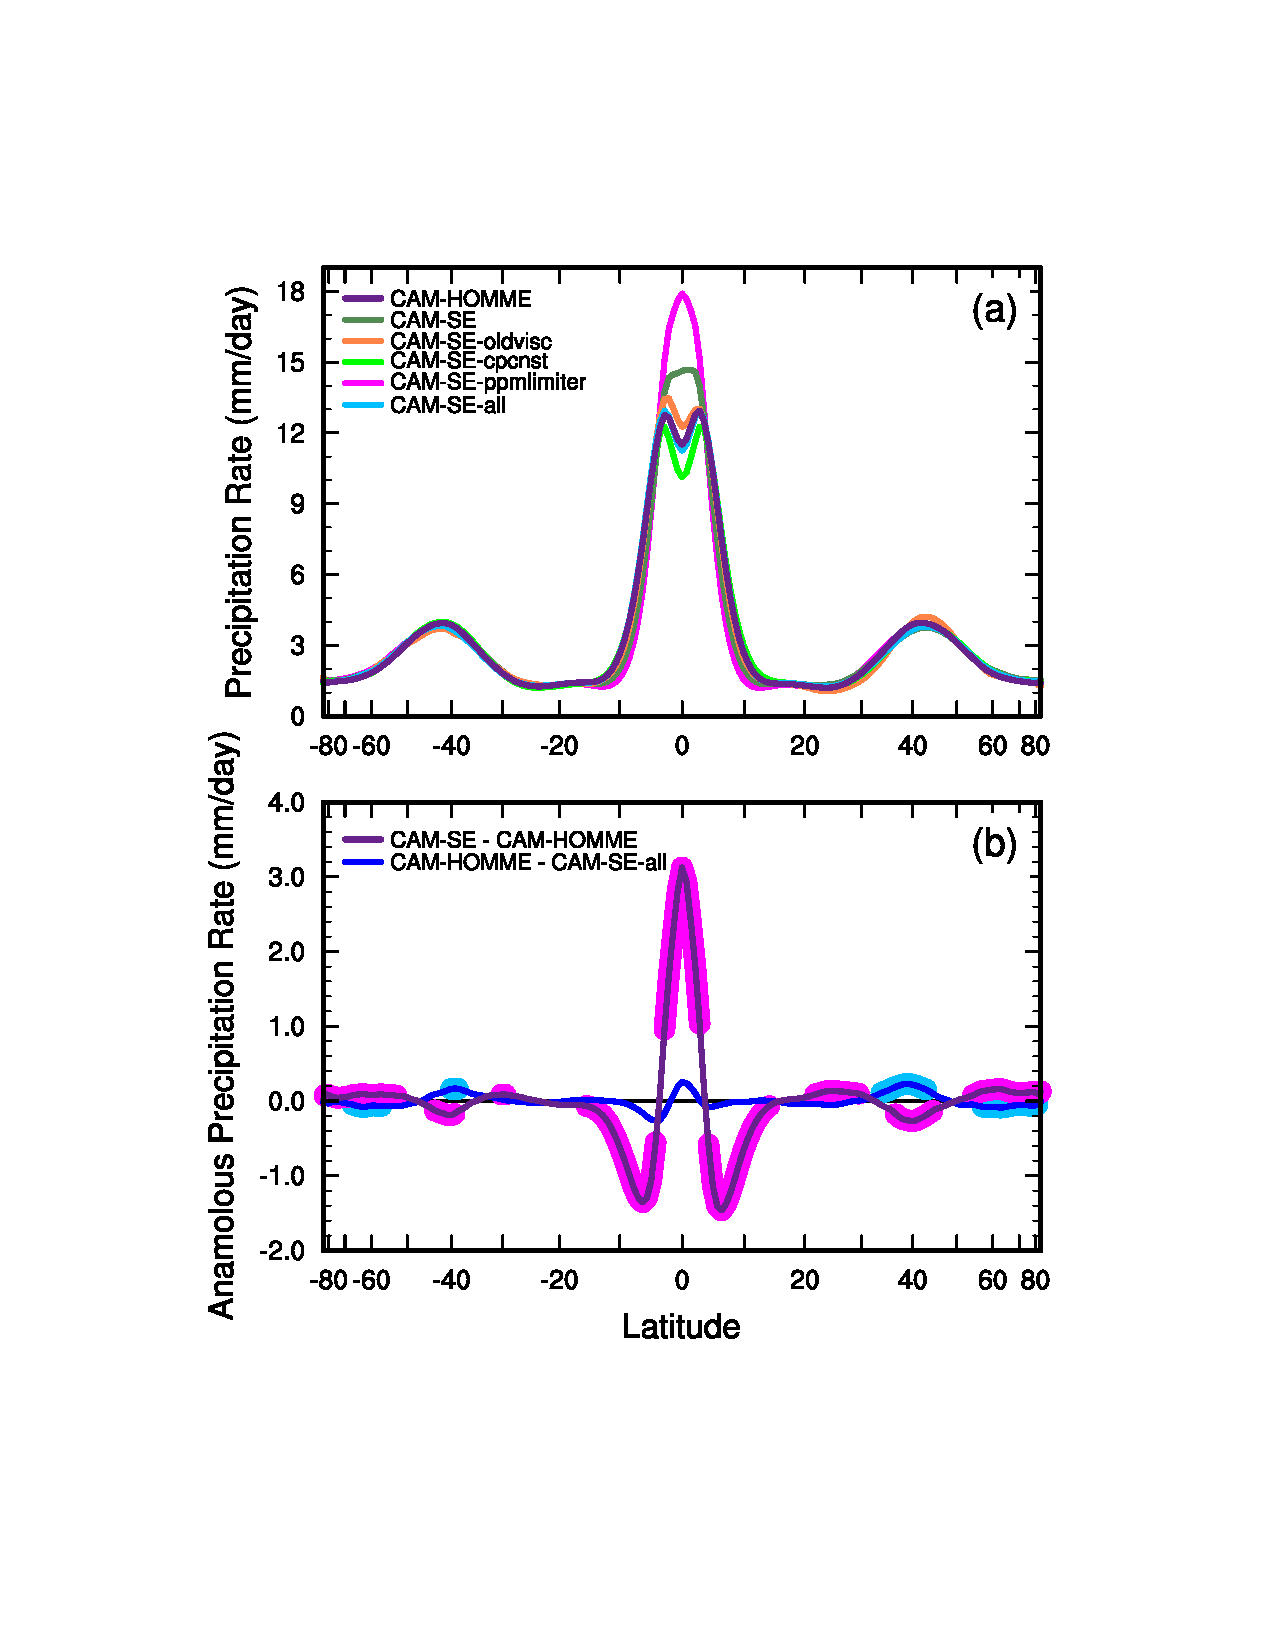
\includegraphics[width=20pc]{figs/dzonal_prect.pdf}
\caption{(A) The zonally averaged total precipitation rates in the aqua-planet simulations, averaged over the final 4 years of a 4.5 years simulation. Labels are defined in the text (B) The change in the total precipitation rate between two simulations denoted by the label. The shading indicates where the differences are significant at the 95\% confidence level.}
\label{fig:dzonal}
\end{figure}

An analysis of the vertically integrated, zonally averaged dry static energy budget indicates that the latent heating due to the change in precipitation rate are balanced by the anomalous dry static energy flux convergence due to the increase in the mean resolved vertical upward motion at the equator (the dynamic component from equation (3) in \cite{MO2011NATUREC}; not shown). This balance also holds for the reduction in precipitation rate on the flanks of the equator (not shown). It is likely that an increase in resolved vertical upward motion in CAM-SE drives the increase in large-scale condensation rate observed in CAM-SE, consistent with a prior analysis of CAM-HOMME \citep{OETAL2016JAMES}. In this scenario, greater downward motion observed on the flanks of the equator are simply compensating for the increased mass flux at the equator, which then acts to stabilize the column and reduce the precipitation rate locally.

The authors have identified three design aspects of CAM-SE that explain the large changes in precipitation observed in the tropics. These three design aspects are: the use of a lower divergence damping coefficient, a thermodynamically consistent definition of $c_p$ (see \eqref{eq:cp}) and the removal of the limiter in the vertical remapping of the horizontal winds. The individual effect of each of the three design choices is illustrated in Figure~\ref{fig:dzonal}a, showing the total precipitation rate from three additional CAM-SE simulations, each simulation having one of the three modifications reverted back to the CAM-HOMME design. By using the larger divergence damping coefficients from CAM-HOMME in CAM-SE ('CAM-SE-oldvisc'), the precipitation rate at the equator is reduced by about 1 mm/day compared with CAM-SE. The CAM-SE simulation in which the limiter is turned on (CAM-SE-ppmlimiter), as it is in CAM-HOMME, results in a dramatic increase in equatorial precipitation of 3-4 mm/day compared with CAM-SE (Figure~\ref{fig:dzonal}a). Through reverting the definition of $c_p$ back to the CAM-HOMME definition ($c_p = c_p^{(d)}$; 'CAM-SE-cpcnst'), the near equatorial precipitation rates are dramatically reduced by 3-4 mm/day (Figure~\ref{fig:dzonal}a). A fourth simulation was performed containing all three of the aforementioned modifications ('CAM-SE-all'). The simulated total precipitation rates in CAM-SE-all are indistinguishable from the CAM-HOMME simulation in the zonal mean (Figure~\ref{fig:dzonal}b).

The influence of the new definition of $c_p$ and the PPM limiter on tropical precipitation are not nearly as intuitive as the influence of the divergence damping coefficient. An increase in divergence damping reduces the overall magnitude of the vertical pressure velocities {\color{red}{(Figure~\ref{fig:pdfvisc})}}, likely explaining the reduction in mean precipitation in that simulation. {\color{red}{It is plausible, however, that a less intuitive relationship between divergence damping and precipitation may emerge in a more realistic configuration, acknowledging that \cite{ZHL2012JAS}}} have reported on a counterintuitive relationship to tropical storm genesis. In our aqua-planet simulations, the ITCZ in part, consists of under-resolved, deep convective towers simulated by the resolved dynamics, consistent with a prior study of CAM-HOMME \citep{HR2017JCLIM}. The base of the convective towers often originate within the boundary layer, with convergent flow driving resolved upward mass fluxes through the cloud base. In the CAM-SE-ppmlimiter simulation, the magnitude of the horizontal velocities in the lowest model level of the equatorial convergence zone are larger (Figure~\ref{fig:schematic}b). The authors speculate that the limiter will select a larger magnitude horizontal wind in the lowest model level in a convergent flow regime, resulting in greater convergence, vertical motion and therefore precipitation.

\begin{figure}[h]
\centering
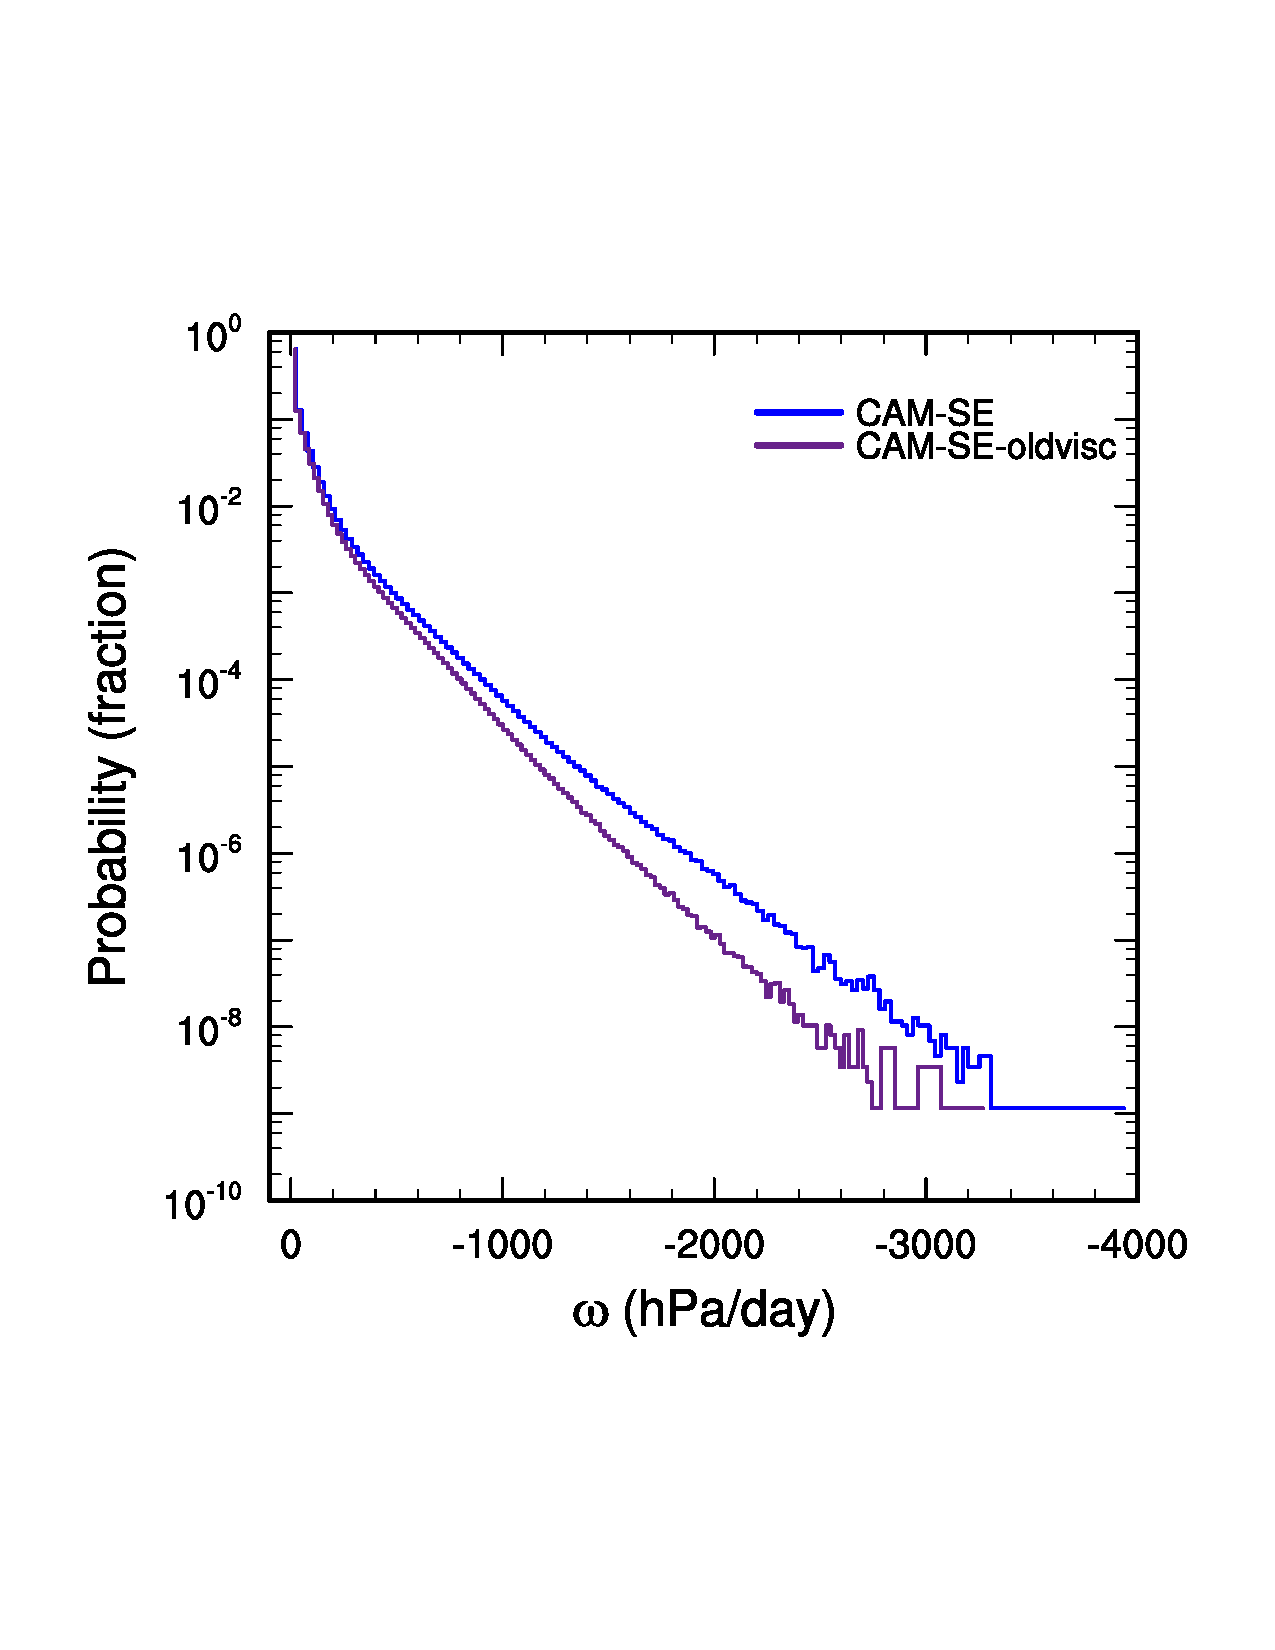
\includegraphics[width=20pc]{figs/temp_pdf_SE_v_SE-oldvisc.pdf}
\caption{{\color{red}{Probability density distribution of the upward vertical pressure velocities ($\omega$), everywhere in the model for CAM-SE and CAM-SE-visc. Figure computed from a single year of six-hourly output. CAM-SE-visc has a divergence damping coefficient 6.25 times that of CAM-SE, resulting in a reduction in the magnitude of $\omega$.}}}
\label{fig:pdfvisc}
\end{figure}

To explain how the limiter may influence mass convergence, consider a vertical profile of the horizontal wind, $u_k$, across the lowest model level, $k=nlev$, and the second lowest model level, $k=nlev-1$ (Figure~\ref{fig:schematic}a). Assume that level $nlev$ is undergoing horizontal mass convergence, which over the course of a vertical remapping time-step, raises the top of the lowest model level. With the limiter off, the value of the wind at the new time-step, $u_{\tilde nlev}$, is evaluated through integrating the sub-grid PPM reconstruction (pink line in Figure~\ref{fig:schematic}a) from the surface to the top of the raised model level, such that the contribution of $u_{nlev-1}$ to $u_{\tilde nlev}$ is shown as the vertical green line in Figure~\ref{fig:schematic}a. The limiter, on the other hand, forces the contribution of $u_{nlev-1}$ to $u_{\tilde nlev}$ to be exactly equal to its previous value of $u_{nlev-1}$. The schematic wind profile in Figure~\ref{fig:schematic}a, indicating mass convergence in a region of positive $du/dz$, is characteristic of the equatorial convergence zones, and through turning the limiter on, increases the magnitude of the lowest level winds by systematically shifting the contribution of the raised level interface to the right in Figure~\ref{fig:schematic}a.

\begin{figure}[h]
\centering
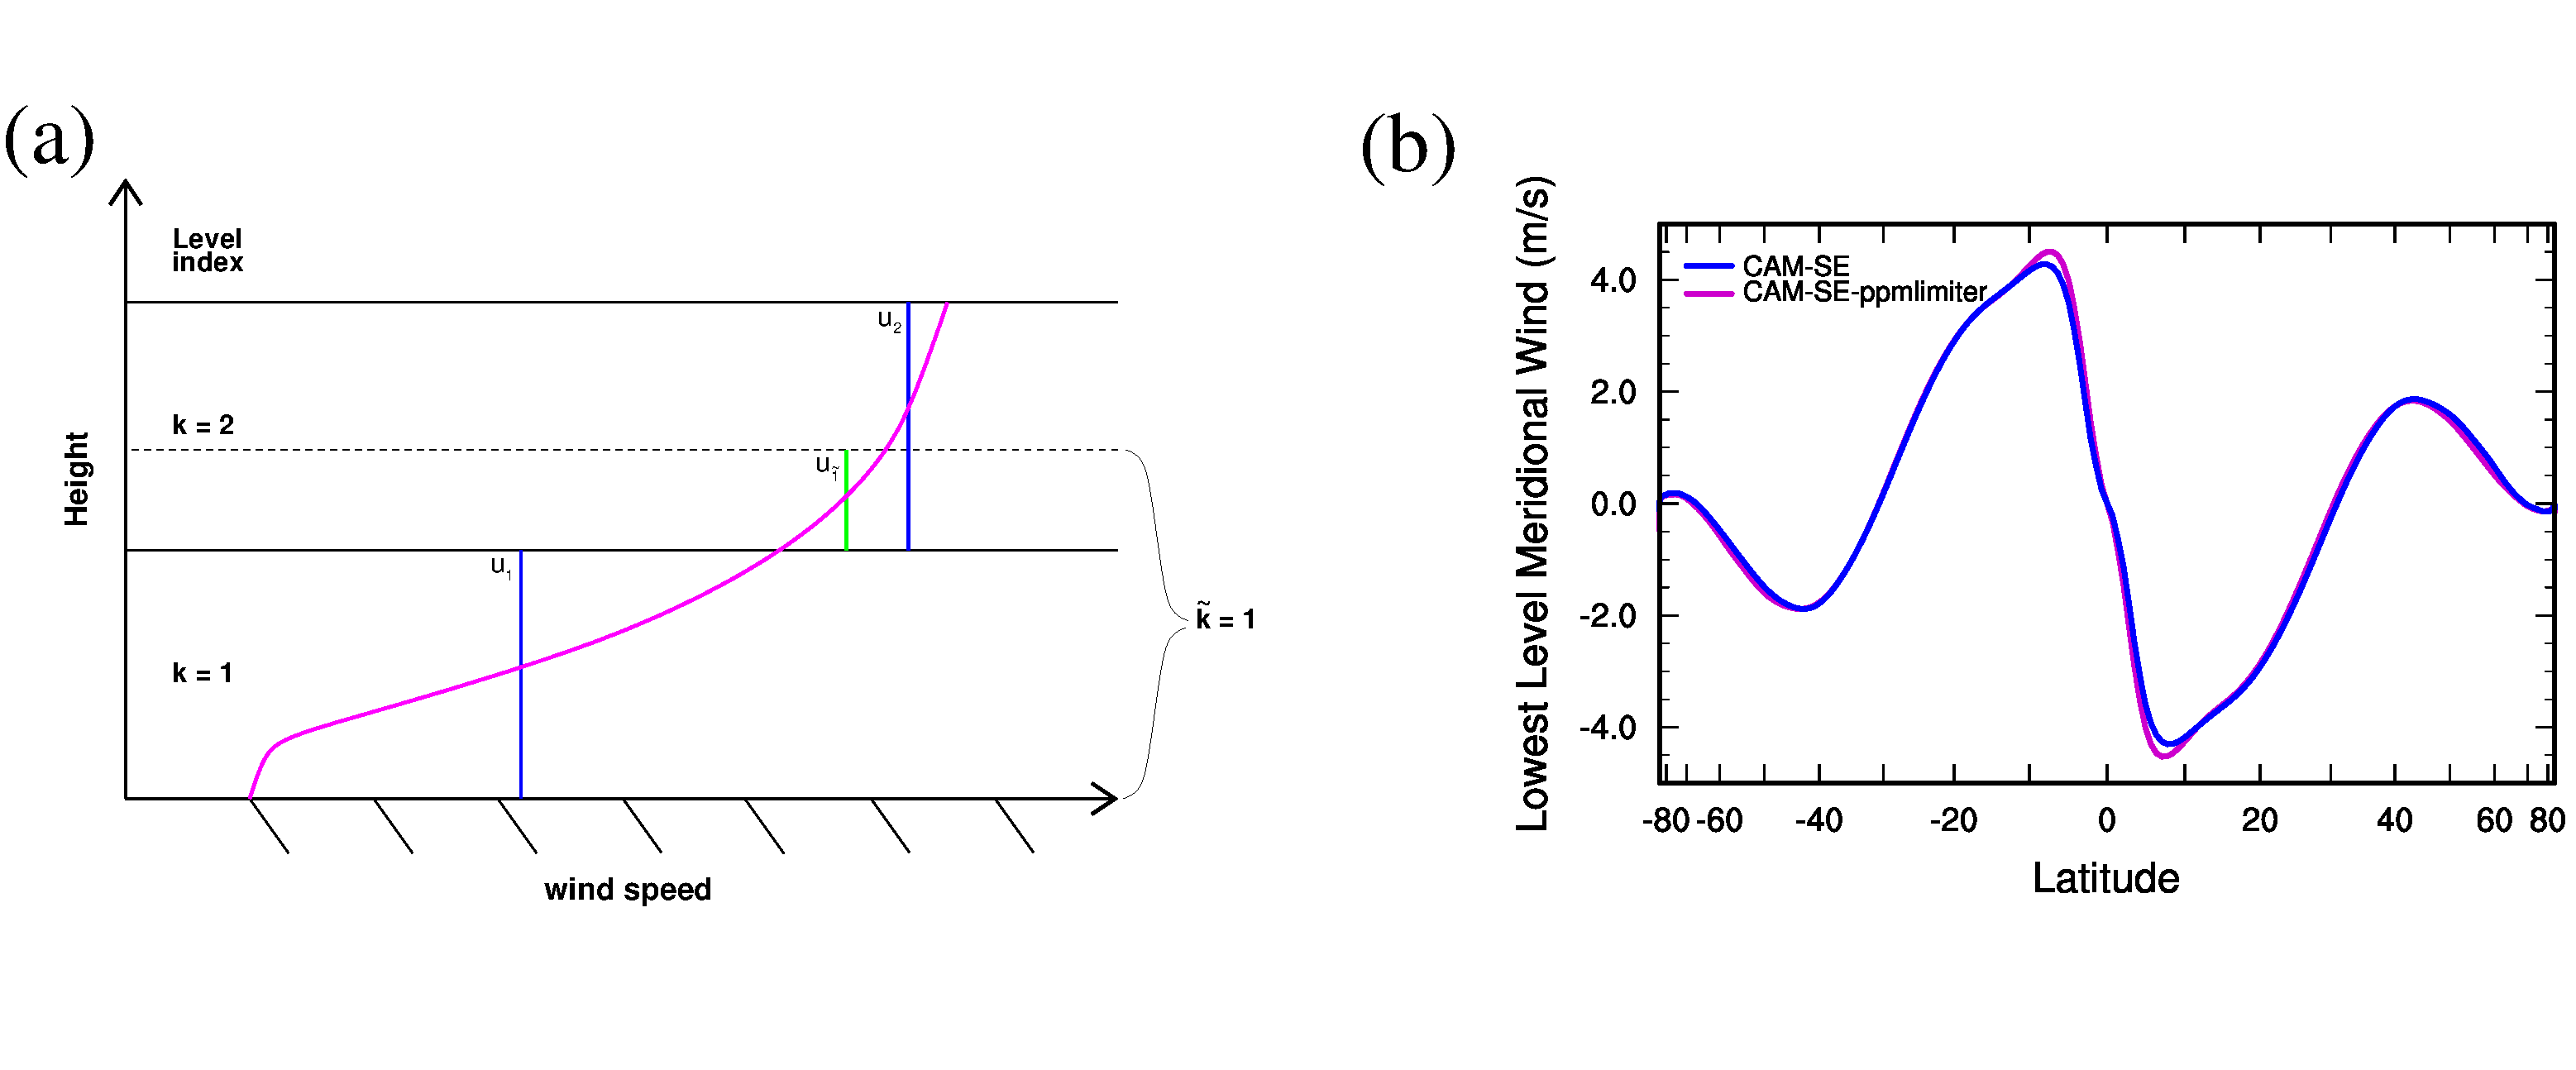
\includegraphics[width=30pc]{figs/schematic.pdf}
\caption{(a) A schematic illustration of the influence of the limiter on the vertical remapping of the winds of the lowest model level, in a convergent flow regime. Solid black lines show the layer interface, and the dashed line shows the top of the lowest model level in the following time-step. The discretized model winds are denoted as blue bars, while the PPM reconstruction is shown as the pink curve. The green bar is the wind computed by integrating the reconstruction from the top of level 1 to the top of level 1 in the following time-step. Notations are provided in the text. (b) Time-mean, zonally averaged lowest model level meridional wind in the CAM-SE and CAM-SE-ppmlimiter simulations, computed from the entirety of a 4.5 year simulation.}
\label{fig:schematic}
\end{figure}

The influence of a thermodynamically consistent definition of $c_p$ is to increase precipitation near the equator by 3-4 mm/day (Figure~\ref{fig:dzonal}a). Note that the $c_p=c_p^{(d)}$ change affects not only the energy conversion term in the thermodynamic equation (equation \eqref{E:PEtemp}) but also the frictional heating term (equation \eqref{eq:tcp}) and the vertical remapping of temperature (section \ref{sec:verticalRemappin}). An additional aqua-planet simulation reveals the frictional heating term has a non-negligible contribution to the $c_p$ sensitivity. A simulation in which $c_p = c_p^{(d)}$ only in the frictional heating term (equation \eqref{eq:tcp}), results in a reduction in equatorial precipitation of 1-2 mm/day (not shown). This result is intuitive, since the term $\left(\mathbf{v}\cdot \delta \mathbf{v}\right)$ is always negative, the heating rate is inversely proportional to $c_p$. In CAM-SE, $c_p$ is always greater than $c_p^{(d)}$, and so there is more frictional heating in CAM-SE than in CAM-HOMME, all other aspects being equal. In the equatorial regions, additional heating likely facilitates buoyancy, which increases resolved vertical motion, leading to an increase in precipitation. 

One of the motivations for moving to a dry-mass vertical coordinate is to make the coupling between the physics and dynamics more consistent. It is generally assumed that pressure surfaces are unchanged across a physics time-step. However, this assumption is often violated when using a moist pressure based vertical coordinate -- a mass source term must be estimated when there is a change in water species due to the physical parameterizations. While the developments presented in this work concludes a significant portion of the effort required to achieve consistent coupling, at present, the CAM physics packages have not yet been made consistent with a dry-mass vertical coordinate. The authors speculate that some of the sensitivity to $c_p$ shown in Figure~\ref{fig:dzonal}a is related to the inconsistent definitions of internal energy between CAM-SE and the physics packages. An inconsistent energy definition between the dynamical core and the physics package can result in inconsistent forcing terms being passed back and forth. It was decided that this complication be left to a future sensitivity analysis, once the physics package has been made consistent with the dry-mass vertical coordinate and a comprehensive treatment of condensates and energy. But as a final point of caution, the authors recognize that while there is a surprising sensitivity of aqua-planet solutions to dynamical core design choices, this sensitivity may be different, or even non-existent, in more realistic Earth-like configurations. These remaining uncertainties are left to be explored in future work.

\subsubsection{Conservation}
To assess the AAM conservation properties of the CAM-SE dynamical core, the diagnostics used in \cite{LBDL2014JAMES} are applied to the Aqua-planet simulation described in Section \ref{sec:APE}. In the dynamical core the column integrated wind and mass AAM are written to history files and the total integrals of AAM are computed as a post-processing step. The torques are obtained by subtracting the global integrals of AAM divided by the time-increment between the outputs of the AAM. For details on the discretized AAM diagnostics see \cite{LBDL2014JAMES}. These diagnostic outputs are part of the CESM2 release and are controlled with namelist variables.

As discussed in Section \ref{sec:aam} the total AAM torque from the dynamical core, in the absence of topography, should be small {\color{red}{(ideally zero)}} compared to the torque from the parameterizations {\color{red}{which is not spurious}}. {\color{red}{CAM-SE uses the vector-invariant form of the momentum equations and the discretization thereof is not inherently AAM conserving. That said, Figure \ref{fig:aam} shows CAM-SE conserves AAM very well:}} The spurious torques from the dynamical core are approximately a factor 100 smaller than the physical torques from the parameterizations. These results are very similar to the dynamical core torques found in the dry Held-Suarez setup used in \citet{LBDL2014JAMES}.

Similarly to the AAM diagnostics, the total column-integrated moist energy is output at various places in the dynamical core and physics parameterizations. The dynamical core conserves the moist total energy, equation \eqref{eq:comprehensice_energy}, to about 0.1$W/m^2$. The frictional heating term described in section \ref{sec:frictional_heating} is approximately 0.4$W/m^2$ and hence an important term for total moist energy conservation. As mentioned in section \ref{sec:aam} the CAM physics energy fixer enforces a different energy than the comprehensive moist energy. This inconsistency should be removed in future CAM versions, however this is not a trivial modification to the CAM physics package. The discrepancy between the two definitions of energy is approximately 0.5$W/m^2$ \citep[similar to what ][ found when just including the correct heat capacity for water vapor in the total energy equation]{T2011LNCSEb}. A detailed energy analysis will be the subject of a future publication.
%
\begin{figure}[h]
\centering
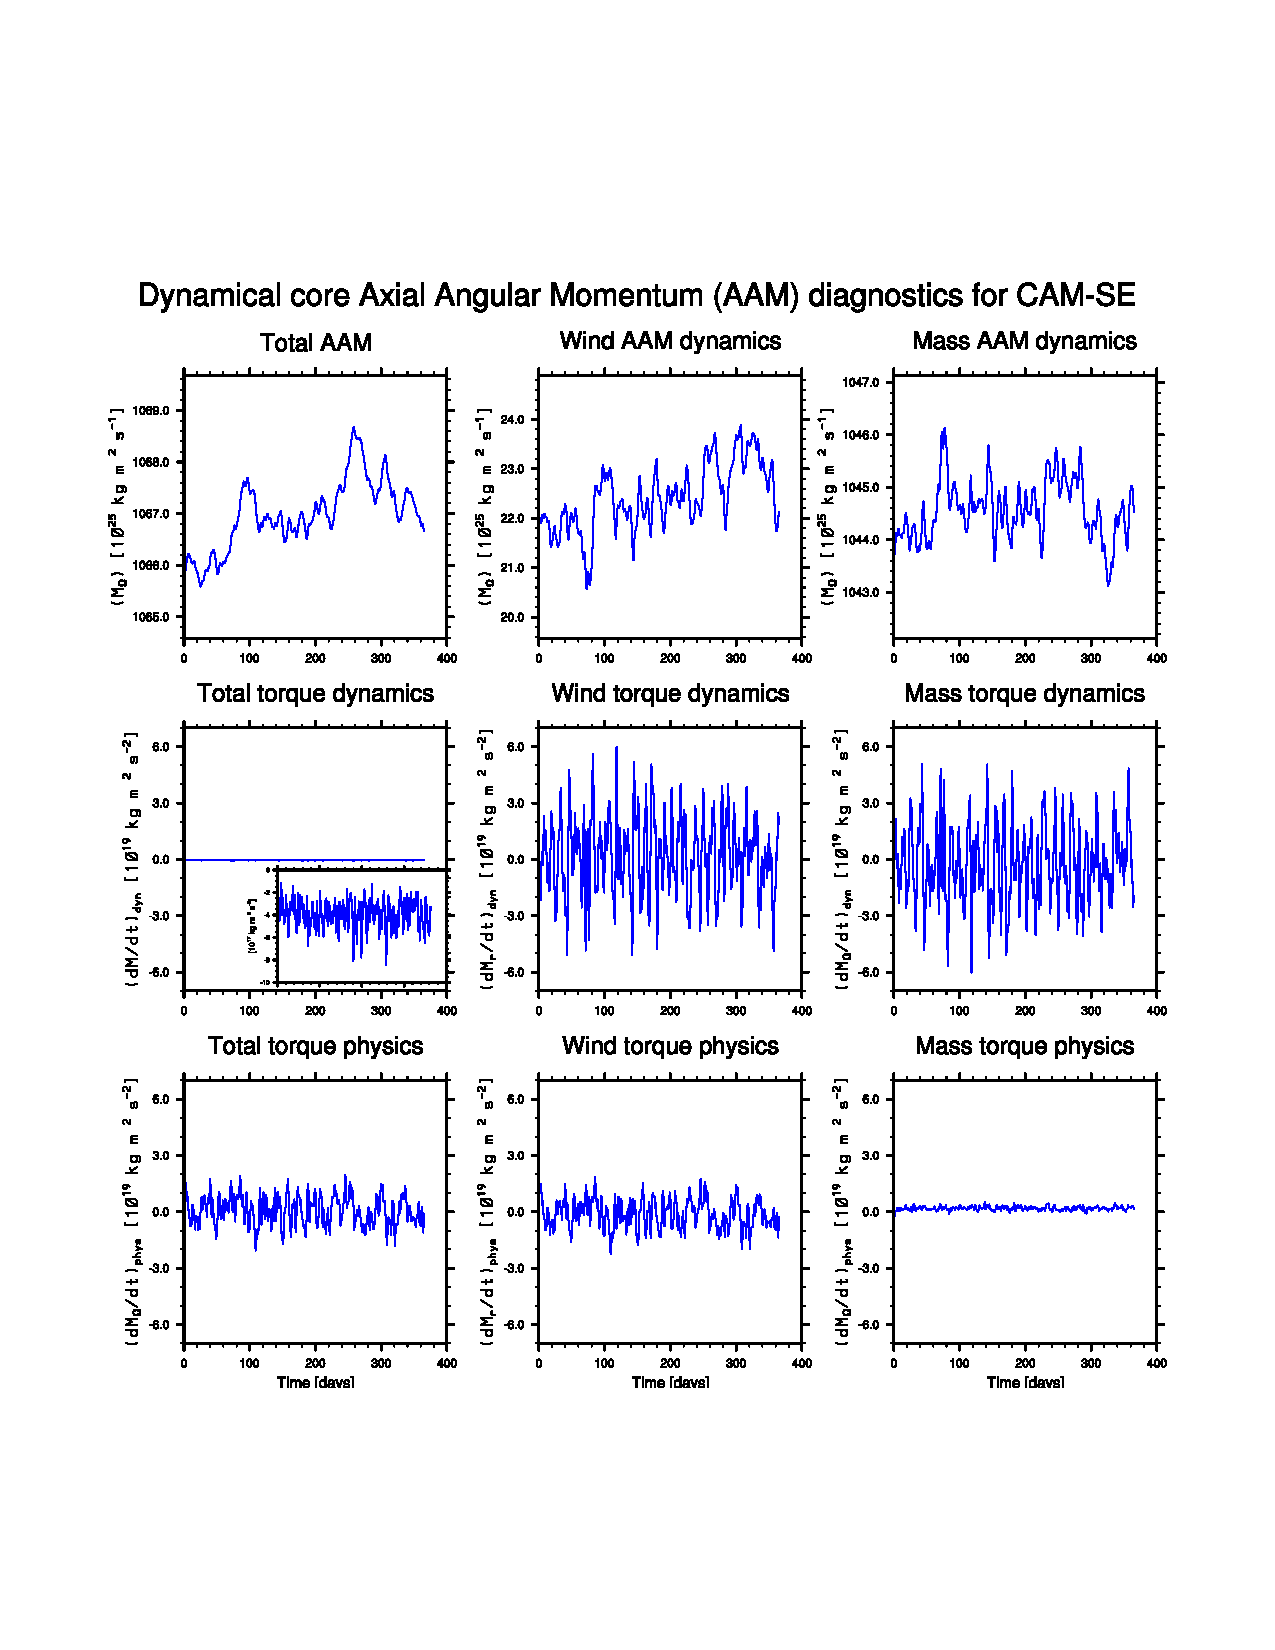
\includegraphics[width=30pc]{figs/aam.pdf}
\caption{The first row shows total (column 1), wind (column 2) and mass (column3) AAM as a function of time for the first year of the CAM6 aqua-planet simulation. The remaining plots show total, wind and mass AAM torques as a function of time (column 1,2,3, respectively) for the dynamical core (row 2) and parameterizations (row 3). Note that it is necessary to enlarge the y-axis of the dynamical core torque by a factor of approximately 100 to visualize the dynamical core torque. Hence the spurious torque from the dynamical core is small compared to the physical torques from the parameterizations.}
\label{fig:aam}
\end{figure}
\subsection{Performance}\label{sec:performance}
In addition to the numerical changes described in the previous section, a number of changes to the computational structure of the SE dynamical core were also made which both reduce the computational cost at both modest and large processor count.  In particular, new communication operators were developed which reduces the amount of data movement between MPI ranks as well as through the memory hierarchy. Derivative operators were optimized to increase code vectorization, and the limiter operator was rewritten to reduce cost.  The CAM-HOMME configuration is referred to as the {\em{original}} codebase and CAM-SE is referred to as the {\em{optimized}} codebase in this section. So when comparing computational cost of CAM-HOMME and CAM-SE it reflects not only the code optimizations but also the numerous science changes in CAM-SE that require extra computational work (e.g., the heat capacity is a function of water loading tracers and therefore not constant, (moist) pressure is not a prognostic variable and must be diagnosed, the reference pressure computation is not in CAM-HOMME).
%A more detailed description of the optimizations can be found in \cite{dennis2017}. 
\begin{figure}[h]
\centering
 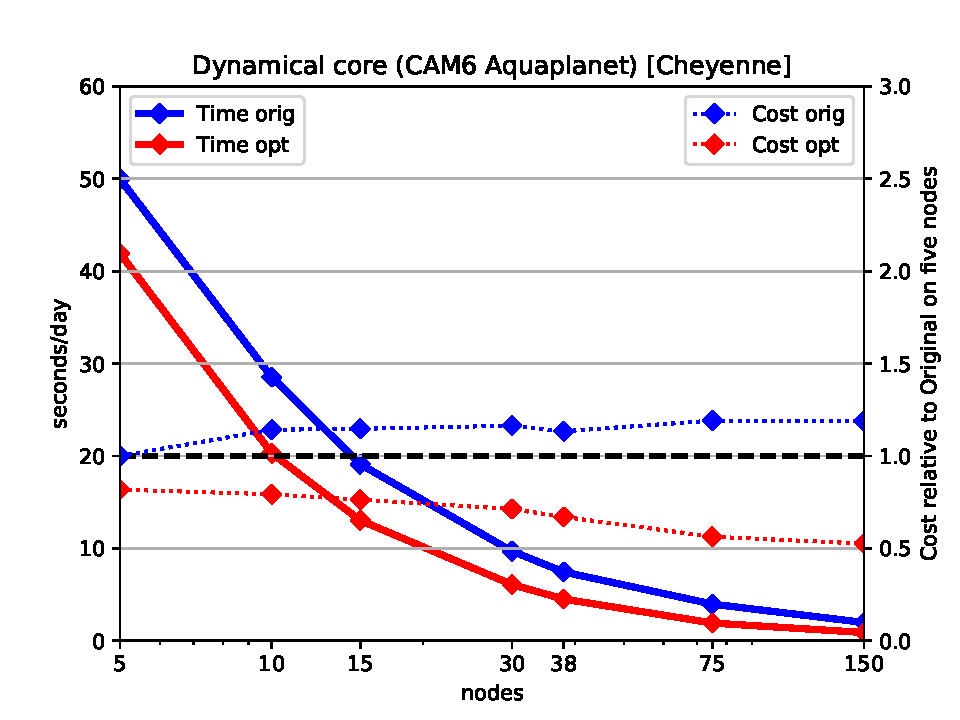
\includegraphics[scale=0.45]{figs/aqua-perf}
 \caption{The execution time of the SE dynamical core in an Aquaplanet configuration using CAM6 physics at $1^\circ$ horizontal resolution on Cheyenne.   Both the original (CAM-HOMME) and optimized code (CAM-SE) is indicated by the solid blue and red lines, while the dotted lines represent the computational cost.}
 \label{fig:aqua-perf}
\end{figure}

We provide the execution time and computational cost on Cheyenne for the dynamical core component for the $1^\circ$ CAM6 Aquaplanet configuration used in Section \ref{sec:APE} ($N_e=30$, $N_p=4$, $nlev=32$). Cheyenne is an SGI ICE Cluster with 4,032 dual-socket Intel Xeon based nodes with 36 cores/nodes.   The x-axis is the number of nodes while the left y-axis corresponds to execution time in seconds/day, and the right y-axis corresponds to the relative computational cost normalized to the original code run on five nodes or 180 cores of Cheyenne. Execution times and computational costs are also provided for up to 150 nodes or 5400 cores where a single spectral element in the horizontal is allocated to each core.

It is clear from Figure \ref{fig:aqua-perf} that the execution time for the dynamical core for the optimized version (CAM-SE) is significantly less than the original codebase (CAM-HOMME) for all core counts. The reduction in execution time for the optimized versus the original code varies from approximately 20\% at small core counts to slightly more than 50\% at larger core counts. The percentage reduction in execution time for the optimized versus original code is readily apparent by looking at the relative computational cost curves indicate by the dotted lines in Figure \ref{fig:aqua-perf}.  A value greater than one indicates that it is more expensive to run a particular configuration than the original code on five nodes, while a value less than one indicates that it is cheaper to run a particular configuration.  This approach allows for the comparison of both the impact of the optimizations have on a particular node code as well as the impact of optimizations to code scalability.  Interestingly while the original code becomes more expensive to execute at larger core counts the optimized code actually becomes cheaper.  In particular, the greatest reduction of 40\% in computational cost occurs on 75 nodes.  We suspect that the decrease in computational cost illustrated in Figure \ref{fig:aqua-perf} is likely due to the fact that the calculations performed in the dynamical core now fit into the Level 3 (L3) cache on 75 nodes where they did not previously i:n either the original code base on the optimized code base on smaller node counts.  The decreased execution time due to the calculations being L3 cache resident is sufficiently large as to overcome any increase in execution time increase due to message passing.  

{\color{red}{The cost of the dynamical core for the optimized code base is compared to other pieces of the Community Atmosphere Model is illustrated in Figure \ref{fig:cost}. We categorize four different pieces of CAM for timing purposes: physics, dynamics, I/O and the remapping of data-structures necessary between the physics and dynamics.  The faction of time that CAM spends performing the dynamics drops from a maximum of 44\% on five nodes, to a minimum of 27\% on 150 nodes.  While there is an increase in the relative cost for both the I/O and physics to dynamics interface, the largest relative increase in cost is seen in the physics calculations after 30 nodes. We suspect that this very modest increase in the cost of the physics is a result of a minor unavoidable load-imbalance of various physics processes. Figure \ref{fig:cost} illustrates that for CAM-SE the number of core-hours per simulated year is quite constant and only varies from a low of 1630 to 1794 over a very large core count range.}}

Note that for this comparison we use the same Aquaplanet CAM6 configuration, which achieves simulation rates that range from a low of {\color{red}{ 2.5}} Simulated years per day (SYPD) on 5 nodes, to {\color{red}{ 62.8}} SYPD on 150 nodes, and run for 1 month (see Figure \ref{fig:SYPD}). This length of simulation includes the default monthly history I/O output as well as the generation of a restart file. A rule of thumb for CESM is that the model should produce a minimum of 20 SYPD to be fast enough for doing 'standard' climate science with the model. CAM-SE achieves this threshold with fewer than 2000 processors. At this processor count CAM-FV exhibits similar throughput (not shown) and with larger processor counts CAM-SE continues to scale well.

\begin{figure}[h]
\centering
 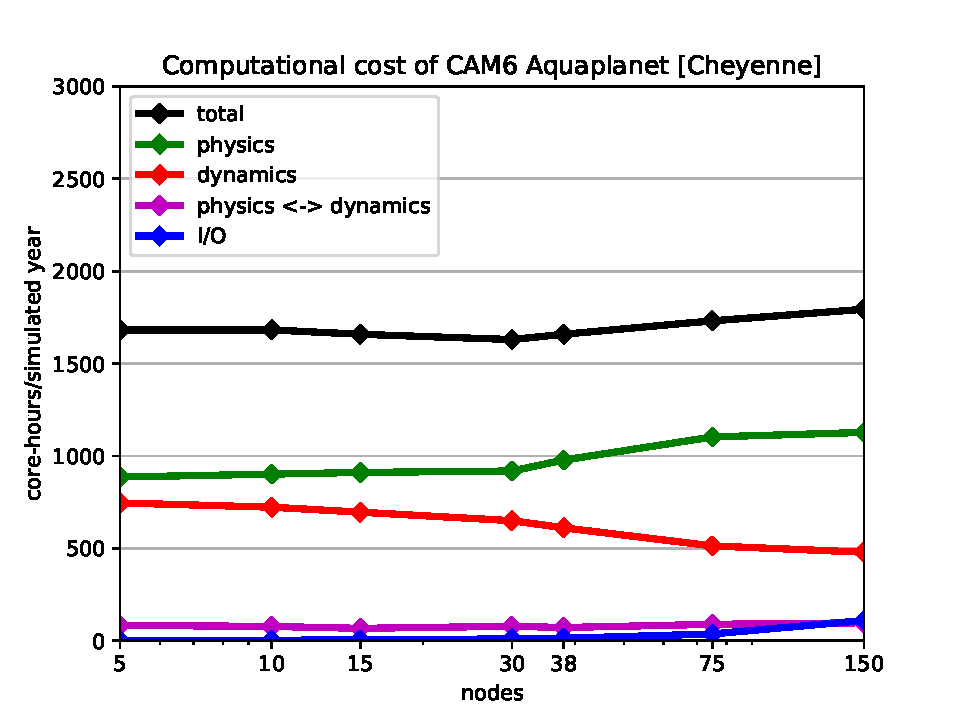
\includegraphics[scale=0.5]{figs/cost}
 \caption{{\color{red} The cost in core-hours per simulated-year is provided for several different sub-components of CAM for the $1^\circ$ horizontal resolution Aquaplanet simulation on Cheyenne (see text for more details).}}
 \label{fig:cost}
\end{figure}
\begin{figure}[h]
\centering
 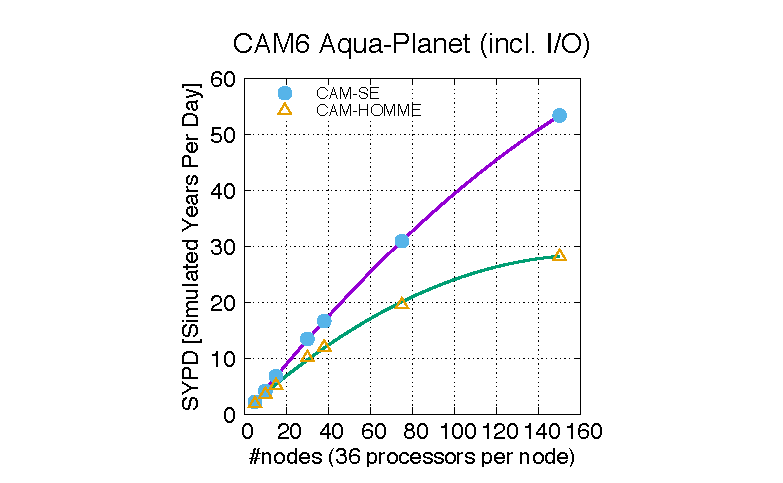
\includegraphics[scale=1.0]{figs/SYPD}
 \caption{Throughput in terms of simulated years per day for CAM6 Aqua-planet including I/O for CAM-SE and CAM-HOMME as a function of number of nodes. The curved line is a parabolic Least-Squares fit to the data points. Note that for the right-most data-point there is only one element in the horizontal per processor (150 nodes is 5400 processors and there are $6\times N_e^2=6\times 30^2=5400$ elements in the horizontal).}
 \label{fig:SYPD}
\end{figure}

%       NEW
%   s:  2.49 SYPD (5 nodes  - 180 cores)
%   m:  4.93 SYPD (10 nodes - 360 cores)
%   l:  7.44 SYPD (15 nodes - 540 cores)
%  xl: 14.94 SYPD (30 nodes - 1080 cores)
% xxl: 18.57 SYPD (38 nodes - 1368 cores)
%  3x: 34.30 SYPD (75 nodes - 2700 cores)
%  4x: 62.76 SYPD (150 nodes- 5400 cores)

%   OLD
%   s:  2.00 SYPD
%   m: 3.69 SYPD
%   l:    5.30 SYPD
% xl:    10.23 SYPD
% xxl:   12.14 SYPD
% 3x:    19.68 SYPD
% 4x:     28.31 SYPD


\section{Conclusions}\label{sec:concl}
The NCAR CESM2.0 version of CAM-SE is presented. This version uses a dry-mass vertical coordinate and has a comprehensive treatment of condensates both in the thermodynamic equation and momentum equations. The conservation properties in terms of total energy and axial angular momentum for this system of equations derived. The discretization of the equations of motion is explained in detail and is intended to serve as a comprehensive documentation for CAM-SE. Idealized simulations demonstrate the accuracy and conservation property of the numerical model. In particular, we show that the reduction in viscosity parameters greatly improved the total kinetic energy spectrum of CAM-SE and that the comprehensive treatment of moist thermodynamics and condensate loading significantly changes precipitation rates in aqua-planet simulations. Last but not least the CAM-SE model has been sped-up significantly (from 20\% to 50\% depending on core count) compared to its predecessor CAM-HOMME.
%Text here ===>>>

%%

%  Numbered lines in equations:
%  To add line numbers to lines in equations,
%  \begin{linenomath*}
%  \begin{equation}
%  \end{equation}
%  \end{linenomath*}



%% Enter Figures and Tables near as possible to where they are first mentioned:
%
% DO NOT USE \psfrag or \subfigure commands.
%
% Figure captions go below the figure.
% Table titles go above tables;  other caption information
%  should be placed in last line of the table, using
% \multicolumn2l{$^a$ This is a table note.}
%
%----------------
% EXAMPLE FIGURE
%
% \begin{figure}[h]
% \centering
% when using pdflatex, use pdf file:
% \includegraphics[width=20pc]{figsamp.pdf}
%
% when using dvips, use .eps file:
% \includegraphics[width=20pc]{figsamp.eps}
%
% \caption{Short caption}
% \label{figone}
%  \end{figure}
%
% ---------------
% EXAMPLE TABLE
%
% \begin{table}
% \caption{Time of the Transition Between Phase 1 and Phase 2$^{a}$}
% \centering
% \begin{tabular}{l c}
% \hline
%  Run  & Time (min)  \\
% \hline
%   $l1$  & 260   \\
%   $l2$  & 300   \\
%   $l3$  & 340   \\
%   $h1$  & 270   \\
%   $h2$  & 250   \\
%   $h3$  & 380   \\
%   $r1$  & 370   \\
%   $r2$  & 390   \\
% \hline
% \multicolumn{2}{l}{$^{a}$Footnote text here.}
% \end{tabular}
% \end{table}

%% SIDEWAYS FIGURE and TABLE 
% AGU prefers the use of {sidewaystable} over {landscapetable} as it causes fewer problems.
%
% \begin{sidewaysfigure}
% \includegraphics[width=20pc]{figsamp}
% \caption{caption here}
% \label{newfig}
% \end{sidewaysfigure}
% 
%  \begin{sidewaystable}
%  \caption{Caption here}
% \label{tab:signif_gap_clos}
%  \begin{tabular}{ccc}
% one&two&three\\
% four&five&six
%  \end{tabular}
%  \end{sidewaystable}

%% If using numbered lines, please surround equations with \begin{linenomath*}...\end{linenomath*}
%\begin{linenomath*}
%\begin{equation}
%y|{f} \sim g(m, \sigma),
%\end{equation}
%\end{linenomath*}

%%% End of body of article

%%%%%%%%%%%%%%%%%%%%%%%%%%%%%%%%
%% Optional Appendix goes here
%
% The \appendix command resets counters and redefines section heads
%
% After typing \appendix
%
%\section{Here Is Appendix Title}
% will show
% A: Here Is Appendix Title
%
\appendix
   \section{Dissipation}\label{sec:dissipation}
   \subsection{Discretization}
   In the CAM-SE model explicit  fourth-order hyperviscosity  ($\nu \nabla^4 \phi$) used as 
    the main stabilization mechanism.  For scalar fields such as $T, p, q$ etc., 
   a scalar viscosity   is applied,  while  for the horizontal momentum equations vector viscosity
   ($\nu \nabla^4 \mathbf{v} $) is employed. The coefficient of viscosity $\nu$ may be constant or a spatially varying 
  quantity  depending on the application. High-order viscosity operator $ \nu \nabla^{2m} \phi$, $m=2,3, \dots$, 
    for an arbitrary variable $\phi$  can be constructed 
  by successively applying the basic Laplacian-type viscosity operator $\nabla^2 ( \,)$. In order to describe the SE discretization 
  we consider the basic Laplacian without the coefficient of viscosity $\nu$: 
   \begin{equation}
   L(\phi)  = \nabla^2 \phi .  \label{eq:Laplace}
   \end{equation}
   %
  Integrating  (\ref{eq:Laplace}) over an element $\Omega_e$  with boundary $\Gamma_e$, using Greens method   results in 
    \begin{equation}
  %
  \int_{\Omega_e}  L \, \psi  \,  d \Omega_e  =   \int_{\Gamma_e}  \phi \nabla \psi  \,    d  \Gamma_e - 
                      \int_{\Omega_e}  \nabla \psi \cdot \nabla \phi \,  d \Omega_e  \label{eq:Lweak}
   \end{equation}
   For the continuous Galerkin (SE) method the boundary integral vanishes ($\psi = 0$ at the element boundaries) 
   and the  {\em  rhs} simplifies to 
   a surface integral.   The tensor gradients in the integrand  can be expressed  in terms of its contravariant  components 
   $(\tilde{F}^1, \tilde{F}^2)$, using (\ref{eq:covcontra}) such that 
 \begin{equation}
    \nabla \psi \cdot \nabla \phi  = \tilde{F}^1  \frac{\partial \psi}{ \partial x^1} +
      \tilde{F}^2  \frac{\partial \psi}{ \partial x^2} , \quad 
  %
    % 
     \left[   \begin{array}{c}
               \tilde{F}^1  \\     \tilde{F}^2
             \end{array}
           \right]
           =
     \mathbf{D}^{-1}  \mathbf{D}^{-T}   \, \left[   \begin{array}{c}
                \partial \phi / \partial x^1  \\ \partial \phi / \partial x^2 
             \end{array}
           \right] 
           \label{eq:Tgrad}.
  \end{equation}
Thus the discretization of the Laplacian for SE method can be obtained by simplifying the integral 
%
 \begin{equation}
   \int_{\Omega_e}  L \, \psi  \,  d \Omega_e  = -   \int_{\Omega_e}  \nabla \psi \cdot \nabla \phi \,  d \Omega_e
    = -  \int_{\Omega_e} \left[  \tilde{F}^1  \frac{\partial \psi}{ \partial x^1} +
      \tilde{F}^2  \frac{\partial \psi}{ \partial x^2}  \right]    d \Omega_e.  \label{eq:Lap0}
  \end{equation}
  %
 As in the case of  (\ref{eq:se6}),  the weak formulation (\ref{eq:Lap0})  can be evaluated  on the standard element   
  using    the polynomial approximations (\ref{eq:se60}) for $\phi, \psi$ on $\Omega_e$ and GLL quadrature rule.
   Further simplification of (\ref{eq:Lap0})  leads to 
 %
   \begin{equation}
     L^e_{kl} =  - ( \widetilde M^e_{kl})^{-1} \left[ 
           \sum_{i=0}^N  J^{(1)}_e(i,l) \,  \tilde{F}^1_{i l} \, D_{ik}^{(1)}\, w_i  w_l  +
           \sum_{i=0}^N  J^{(2)}_e(k, i) \,  \tilde{F}^2_{k i} \, D_{l i}^{(2)} \, w_k  w_i  \right], 
           \label{eq:Lap1}
   \end{equation}
 where $L^e_{kl}$ is the value of Laplacian term for a grid point $(k,l)$ on $\Omega_e$.  
 
 
   Note that in practice,
 the contravariant gradient terms in  (\ref{eq:Tgrad}) are fist  computed using collocation differentiation,   
 then  the weak  divergence of the gradients   is computed;    this is followed by a  DSS operation which 
 yields the discrete Laplacian ($ L(\phi^e)  \Rightarrow  div(grad(\phi^e))$). 
 
 In CAM-SE the vector viscosity is handled  using the vector Laplacian $\nu \nabla^2 \mathbf{v}$, 
 which is consistent with the curvilinear formulation of the momentum equation.  By using the vector identity 
 $\nabla^2 \mathbf{v} = \nabla(\nabla \cdot \mathbf{v}) - \nabla \times (\nabla \times \mathbf{v}) $, 
 the coefficient of viscosity $\nu$ may be split into the viscosity corresponding to the divergence part $\nu_{div}$
 and that for  the vorticity part $\nu_{vor}$ such that 
 %
 \begin{equation}
  \nu \nabla^2 \mathbf{v} = \nu_{div} \, \nabla(\nabla \cdot \mathbf{v}) -
   \nu_{vor} \,  \nabla \times (\nabla \times \mathbf{v}). \label{eq:vLap}
 \end{equation}
   %
   The SE discretization  of (\ref{eq:vLap}) is handled separately for each component using a vector test function
   $\vec{ \psi}$ and the weak formulation: 
   %
   \begin{eqnarray}
       \nu_{div}  \int_{\Omega_e} \vec{\psi} \cdot   \nabla(\nabla \cdot \mathbf{v})  \,    d \Omega_e  & = & 
       -  \nu_{div} \, \int_{\Omega_e} (\nabla \cdot \vec{\psi})   (\nabla \cdot \mathbf{v})   d \Omega_e \\
         -   \nu_{vor}  \int_{\Omega_e}     \vec{\psi} \cdot  \nabla \times (\nabla \times \mathbf{v})   \,    d \Omega_e  & = &
                          -   \nu_{vor}  \int_{\Omega_e} (\nabla \times      \vec{\psi} ) \cdot (\nabla \times \mathbf{v})    \,     d \Omega_e ,  
   \end{eqnarray}
   where the line integrals along the boundaries associated with weak formulation  vanishes for SE discretization. 
   The {\em rhs} of the above equations are converted into equivalent tensor form  for the divergence and curl terms,
   and discretized as in the case of (\ref{eq:Lap1}). 
   
\subsection{Reference pressure for dry-mass layer thickness damping}\label{app:ref_dp}
Applying $\nabla^4$ damping to $\left( \frac{\partial M^{(d)}}{\partial \eta^{(d)}}\right)$ values directly leads to non-physical model behavior in that physically meaningful gradients in level thicknesses along model surfaces are suppressed, particularly in the vicinity of topography. As an alternative to computing and applying the necessary correction terms to the damping operator, we construct smooth reference values which convey these gradients and apply the damping only to the deviations from these values. Since they are immune from damping processes and can have a significant effect on model behavior, these values must be as accurate as possible and should not impose any predetermined structure. The area weighted averages for each element are least affected by small scale errors and thereby contain the most accurate information available. However, directly computed element averages of $\left( \frac{\partial M^{(d)}}{\partial \eta^{(d)}}\right)$ cannot be used to determine the desired reference values. Averages of this variable or any other variable that cannot be adequately represented as a local linear function of height will contain a systematic bias in the vicinity of topography. To avoid this bias, which varies with $\left| \nabla \Phi\right|$, the reference values must be constructed from other available information. In the following, let $\langle \cdot \rangle$ denote element average values or derived values consistent with computed element averages, and let $M^{(d)}$ denote the weight of dry air per unit area.

To obtain $\left( \frac{\partial M^{(d)}}{\partial \eta^{(d)}}\right)^{(ref)}$, we begin by smoothly interpolating $\langle \Phi \rangle$, $\langle \Phi_s \rangle$, and $\langle T \rangle$ values onto the model grid points. From these, the corresponding average pressure-related values are constructed in two steps using the hydrostatic equation for dry air \eqref{eq:dry_atm_hydro}. First, define the function
\begin{equation}
\mu_k \equiv \frac{1}{\langle M^{(d)} \rangle} \left( \frac{\partial \langle M^{(d)}\rangle}{\partial \eta^{(d)}}\right)_k,
\end{equation}
and iterate from the surface upward to determine its values for each model layer
\begin{equation}
\mu_k=\frac{2\left( \langle \Phi \rangle_k-\langle \Phi \rangle_{k+1/2} \right)}{R^{(d)}\langle T \rangle_k},
\end{equation}
where $\langle \Phi \rangle_{nlev+1/2}=\langle \Phi_s \rangle$. Then iterate downward from the model top to determine the pressure values,
\begin{align}
\left( \frac{\partial \langle M^{(d)}\rangle}{\partial \eta^{(d)}}\right)_k &= \langle M^{(d)} \rangle_{k-1/2}\left( \frac{2\mu_k}{2-\mu_k}\right),\\
\langle M^{(d)} \rangle_{k}&=\langle M^{(d)} \rangle_{k-1/2}\left( \frac{2}{2-\mu_k}\right),\\
\langle M^{(d)} \rangle_{k+1/2}&=\langle M^{(d)} \rangle_{k-1/2}\left( \frac{2+\mu_k}{2-\mu_k}\right),
\end{align}
where $\langle M^{(d)} \rangle_{1/2}=M^{(d)}_t$ and  $\langle M^{(d)} \rangle_{nlev+1/2}=\langle M^{(d)}_s \rangle$. At this point, we have a set of self-consistent element average values which satisfy the hydrostatic equation
\begin{equation}
\frac{\partial \langle \Phi \rangle}{\partial \eta^{(d)}}=-\frac{R^{(d)}\langle T\rangle}{\langle M^{(d)}\rangle}\left( \frac{\partial \langle M^{(d)}\rangle}{\partial \eta^{(d)}}\right).
\end{equation}
These averages are not suitable for direct use as reference surface values because at the lower boundary they are consistent with the element average of surface geopotential $\langle \Phi_s \rangle$, not with the actual $\Phi_s$ values. To obtain the appropriate reference values corresponding to $\Phi_s$, first adjust the surface pressures
\begin{equation}
\left( M^{(d)}_s \right)^{(ref)}=\langle M^{(d)}_s \rangle\left[ 1+\frac{1}{\langle T\rangle}\frac{\partial \langle T\rangle}{\partial \langle \Phi \rangle}\left( \Phi_s-\langle \Phi_s\rangle \right)\right]^{-\frac{1}{R^{(d)}\frac{\partial \langle T\rangle}{\partial \langle \Phi \rangle}}}\text{ for }\left( \frac{\partial \langle T\rangle}{\partial \langle \Phi \rangle}\right)_{nlev}\neq 0,
\end{equation}
and
\begin{equation}
\left( M^{(d)}_s \right)^{(ref)}=\langle M^{(d)}_s \rangle e^{-\left( \frac{\Phi_s-\langle \Phi_s\rangle}{R^{(d)}\langle T \rangle}\right)}\text{ for }\left( \frac{\partial \langle T\rangle}{\partial \langle \Phi \rangle}\right)_{nlev}= 0.
\end{equation}
Then use the resulting change in weight of dry air per unit area at the surface to determine the reference values for dry-mass thicknesses
\begin{equation}
\left( \frac{\partial M^{(d)}}{\partial \eta^{(d)}}\right)^{(ref)}_k=\left( \frac{\partial \langle M^{(d)}\rangle}{\partial \eta^{(d)}}\right)_k+\left( \frac{\partial B}{\partial \eta^{(d)}}\right)_k\left[ \left( M^{(d)}_s \right)^{(ref)}-\langle M^{(d)}_s \rangle \right],
\end{equation}
where $B$ is the hybrid coefficient.
%
%
% 
\subsection{Hyperviscosity coefficients}\label{app:nu}
The following hyperviscosity coefficients are used in CAM-SE:
\begin{align}
%\nu_T = \nu_{vor} &= 0.2\times \left(\frac{9\times 10^6}{N_e (N_p-1)}\right)^3\, \frac{m^4}{s},\\
%\nu_p = \nu_{div} &= 1.0\times \left(\frac{9\times 10^6}{N_e (N_p-1)}\right)^3\, \frac{m^4}{s},
\nu_T = \nu_{vor} &= 0.150\times \left(\frac{30}{N_e}1.1\times 10^5\right)^3\, \frac{m^4}{s},\\
\nu_p = \nu_{div} &= 0.751\times \left(\frac{30}{N_e}1.1\times 10^5\right)^3\, \frac{m^4}{s},
\end{align}
where $N_e=30$ and $N_e=120$ for the $1^\circ$ and $1/4^{\circ}$ horizontal resolution configurations. Note that mass-wind consistency may be violated if $\nu_p \neq \nu_q$ where $nu_q$ is the viscosity coefficient for tracers. The term inside the parenthesis is the average grid spacing in kilometers and the scaling with resolution is what is used with MPAS \citep[Model for Prediction Across Scales; ][]{SPKS2014JAS}. The damping of temperature and vorticity in CAM-SE is similar to the damping in MPAS, i.e. MPAS uses a coefficient of 0.05 in front of the $(\cdot)^3$ term and CAM-SE uses 0.751.

In the top three levels (sponge layer) the prognostic variables are damped with a Laplacian damping (second-order viscosity)
\begin{equation}
\nu_T = \nu_{vor} = \nu_{div} = \nu_p = 
\begin{cases}
4\times 2.5 \frac{m^2}{s}&, \text{ for }k=1,\\
2\times 2.5 \frac{m^2}{s}&, \text{ for }k=2,\\
1\times 2.5 \frac{m^2}{s}&, \text{ for }k=3,\\
\end{cases}
\end{equation}
for resolutions up to (and including) $N_e=120$.
%
\section{Global conservation}\label{app:conservation}
Below it is shown that the continuous equations of motion, that include the effect of condensates, conserve AAM and total energy. For the derivations first note that adding the continuity equations $\ell \in \mathcal{L}_{all} $ \eqref{E:PEq}, using hydrostatic balance \eqref{eq:phi_1} and ideal gas law \eqref{eq:igl}, yields a moist air continuity
\begin{equation}
\frac{\partial }{\partial t}\left[ \rho \left(\frac{\partial z\quad}{\partial \eta^{(d)}}\right)\right]+\nabla_{\eta^{(d)}} \cdot \left[ \mathbf{v}\rho  \left( \frac{\partial z\quad }{\partial \eta^{(d)}}\right)\right]=0,\label{eq:cont2}
\end{equation}
or, equivalently, in Lagrangian form
\begin{equation}
\frac{d}{dt}\left[ \rho \left( \frac{\partial z\quad }{\partial \eta^{(d)}}\right)\delta A\right]=0,\label{eq:lagra_cont}
\end{equation}
where $\delta A$ is a horizontal area of a Lagrangian air parcel so that $\nabla_{\eta^{(d)}} \cdot \mathbf{v}=\frac{1}{\delta A}\frac{d}{dt}\left( \delta A\right)$, and  $\frac{d}{dt}=\frac{\partial }{\partial t}+\mathbf{v}\cdot \nabla_{\eta^{(d)}} $ is the material/total derivative. 
\subsection{Axial angular momentum (AAM)}
The conservation law for angular momentum is derived in spherical coordinates for which the zonal momentum equation takes the form
\begin{equation}
\frac{du}{dt}=\frac{u v \tan \varphi}{r}+2\Omega v\sin \varphi -\frac{1}{\rho r \cos \varphi}\frac{\partial p}{\partial \lambda},\label{eq:tmp200}
\end{equation}
where $u$ and $v$ are the zonal and meridional velocity components, respectively, $\varphi$ is latitude and $\lambda$ longitude, $\Omega$ rotation rate of Earth ($f=2\Omega \sin \varphi$), and $r$ is the mean radius of Earth.\\

The conservation law for AAM, $\mathcal{M}=\left( u+\Omega r \cos \varphi \right) r \cos \varphi$, can be conveniently derived using the Lagrangian form. Consider the material derivative of $\mathcal{M}$ multiplied by the volume of a Lagrangian air parcel, $\rho \left( \frac{\partial z\quad }{\partial \eta^{(d)}}\right)\delta A$
\begin{equation}
\frac{d}{dt}\left[ \rho \left( \frac{\partial z\quad }{\partial \eta^{(d)}}\right) \delta A \left( u+\Omega r \cos \varphi \right) r \cos \varphi\right].
\end{equation}
Using the chain rule, continuity equation on the form \eqref{eq:lagra_cont}, the equality $v=r\frac{d\varphi}{dt}$ and substituting \eqref{eq:tmp200}, one can obtain an evolution equation for AAM
\begin{equation}
\frac{d}{dt}\left[ \rho \left( \frac{\partial z\quad }{\partial \eta^{(d)}}\right) \delta A\, \mathcal{M} \right]=- \left( \frac{\partial z\quad }{\partial \eta^{(d)}}\right) \frac{\partial p}{\partial \lambda},\label{eq:tmp201}
\end{equation}
or, equivalently, in Eulerian form
\begin{equation}
\frac{\partial}{\partial t}\left[ \rho \left( \frac{\partial z\quad }{\partial \eta^{(d)}}\right) \, \mathcal{M} \right]+\nabla_{\eta_d}\cdot \left[\mathbf{v} \rho \left( \frac{\partial z\quad }{\partial \eta^{(d)}}\right)  \mathcal{M} \right]=- \left( \frac{\partial z\quad }{\partial \eta^{(d)}}\right) \frac{\partial p}{\partial \lambda}.\label{eq:tmp202}
\end{equation}
Repeatedly using the chain rule one can show that the right-hand side of \eqref{eq:tmp201} and \eqref{eq:tmp202} can be written as
\begin{align}
- \left( \frac{\partial z\quad }{\partial \eta^{(d)}}\right)\frac{\partial p}{\partial \lambda}&=-\frac{\partial }{\partial \lambda}\left[  \left( \frac{\partial z\quad }{\partial \eta^{(d)}}\right) p\right]+p\frac{\partial }{\partial \lambda} \left( \frac{\partial z\quad }{\partial \eta^{(d)}}\right)\\ 
&=-\frac{\partial \quad}{\partial \eta^{(d)}}\left( \frac{\partial z}{\partial \lambda}p\right)+\left( \frac{\partial z\quad }{\partial \eta^{(d)}}\right)\frac{\partial p}{\partial \lambda}+p\frac{\partial }{\partial \lambda}\left( \frac{\partial z\quad }{\partial \eta^{(d)}}\right),\\
&=-\frac{\partial \quad}{\partial \eta^{(d)}}\left( \frac{\partial z}{\partial \lambda}p\right)+\left( \frac{\partial z\quad }{\partial \eta^{(d)}}\right)\frac{\partial p}{\partial \lambda}-\frac{\partial }{\partial \lambda}\left[ p\left( \frac{\partial z\quad }{\partial \eta^{(d)}}\right)\right]-\frac{\partial p}{\partial \lambda}\left( \frac{\partial z\quad }{\partial \eta^{(d)}}\right).\\
&=-\frac{\partial \quad}{\partial \eta^{(d)}}\left( \frac{\partial z}{\partial \lambda}p\right)-\frac{\partial }{\partial \lambda}\left[ p\left( \frac{\partial z\quad }{\partial \eta^{(d)}}\right)\right].\label{eq:tmp203}
\end{align}
Substituting \eqref{eq:tmp203} on the right-hand side of \eqref{eq:tmp202} and integrating \eqref{eq:tmp202} in the horizontal and vertical we results in the final AAM equation \eqref{eq:aam_final} in the main text.
\subsection{Total energy}
The derivation of the total energy equation closely follows \citet{K1974MWR} but for a dry mass vertical coordinate and inclusion of condensates in the equations of motion. The equation for the horizontal kinetic energy per unit mass, $K=\frac{1}{2}\mathbf{v}\cdot \mathbf{v}$, is derived by multiplying the momentum equations \eqref{E:PEmom} with $\rho \mathbf{v} \left( \frac{\partial z\quad }{\partial \eta^{(d)}}\right)$ and the continuity equation \eqref{eq:cont2} with $K$, adding the two resulting equations and simplifying using the chain rule yields
\begin{equation}
\frac{\partial }{\partial t}\left[ \rho \left( \frac{\partial z\quad }{\partial \eta^{(d)}}\right)K\right]+\nabla_{\eta^{(d)}} \left[ \rho \mathbf{v} \left( \frac{\partial z\quad }{\partial \eta^{(d)}}\right)K\right]=-\left( \frac{\partial z}{\partial \eta^{(d)}}\right)\mathbf{v} \nabla_{\eta^{(d)}}p-g\rho \left( \frac{\partial z}{\partial \eta^{(d)}}\right)\mathbf{v} \cdot \nabla_{\eta^{(d)}}z.\label{eq:K}
\end{equation}
For the derivation of a flux-form version of the total energy equation (that includes a geopotential term) we substitute
\begin{align}
g \rho \left( \frac{\partial z\quad }{\partial \eta^{(d)}}\right) \mathbf{v} \cdot \nabla_{\eta^{(d)}} z &= \nabla_{\eta^{(d)}}\cdot \left[ gz\mathbf{v}\rho  \left( \frac{\partial z\quad }{\partial \eta^{(d)}}\right) \right] - gz \nabla_{\eta^{(d)}} \cdot \left[ \mathbf{v}\rho  \left( \frac{\partial z\quad }{\partial \eta^{(d)}}\right) \right],\\
&=\nabla_{\eta^{(d)}}\cdot \left[ g z\mathbf{v}\rho  \left( \frac{\partial z\quad }{\partial \eta^{(d)}}\right) \right] -z \nabla_{\eta^{(d)}}\cdot \left[ \mathbf{v} \left( \frac{\partial p\quad }{\partial \eta^{(d)}}\right)\right],\label{eq:tmpK}
\end{align}
(where the hydrostatic balance equation \eqref{eq:phi_1} has been used on the right-hand side of \eqref{eq:tmpK}) on the right-hand side of \eqref{eq:K} and rearrange terms
\begin{equation}
\frac{\partial }{\partial t}\left[ \rho \left( \frac{\partial z\quad }{\partial \eta^{(d)}}\right)K\right]+\nabla_{\eta^{(d)}} \cdot \left[ \rho \mathbf{v} \left( \frac{\partial z\quad }{\partial \eta^{(d)}}\right) \left( K+gz \right) \right]=-\left( \frac{\partial z}{\partial \eta^{(d)}}\right)\mathbf{v} \nabla_{\eta^{(d)}}p - z \nabla_{\eta^{(d)}}\cdot \left[ \mathbf{v} \left( \frac{\partial p\quad }{\partial \eta^{(d)}}\right)\right].\label{eq:tmp1}
\end{equation}
Now, by multiplying the thermodynamic equation \eqref{E:PEtemp} with $\rho \frac{\partial z\quad }{\partial \eta^{(d)}}c_p$ and the continuity equation \eqref{eq:cont2} with $c_p T$, adding the resulting equations and simplifying using the chain rule yields
\begin{equation}
\frac{\partial }{\partial t}\left[ \rho \left( \frac{\partial z\quad }{\partial \eta^{(d)}}\right)c_p T\right]+\nabla_{\eta^{(d)}} \left[ \rho \mathbf{v} \left( \frac{\partial z\quad }{\partial \eta^{(d)}}\right)c_p T\right]=\left( \frac{\partial z\quad}{\partial \eta^{(d)}}\right)\omega.\label{eq:tmp2}
\end{equation}
By using that $\omega\equiv \frac{\partial p}{\partial t}+\mathbf{v} \cdot \nabla_{\eta^{(d)}} p$, using the chain rule and the continuity equation \eqref{eq:cont2} , one can show that
\begin{equation}
\left( \frac{\partial z\quad}{\partial \eta^{(d)}}\right)\omega = \frac{\partial}{\partial \eta^{(d)}}\left( z\frac{\partial p}{\partial t}\right)+\left( \frac{\partial z}{\partial \eta^{(d)}}\right)\mathbf{v} \nabla_{\eta^{(d)}}p +z \nabla_{\eta^{(d)}}\cdot \left[ \mathbf{v} \frac{\partial p\quad }{\partial \eta^{(d)}}\right].\label{eq:tmp3}
\end{equation}
Substituting \eqref{eq:tmp3} on the right-hand side of \eqref{eq:tmp2} and adding the resulting equation to \eqref{eq:tmp1}, the two terms on the right-hand side of \eqref{eq:tmp1} cancel the two last terms on the right-hand side of \eqref{eq:tmp3} and we get the total energy equation
\begin{equation}
\frac{\partial }{\partial t}\left[ \rho \left( \frac{\partial z\quad }{\partial \eta^{(d)}}\right)\left(K+c_pT\right)\right]+\nabla_{\eta^{(d)}} \left[ \rho \mathbf{v} \left( \frac{\partial z\quad }{\partial \eta^{(d)}}\right) \left( K+gz+c_pT \right) \right]=\frac{\partial}{\partial \eta^{(d)}}\left( z\frac{\partial p}{\partial t}\right).\label{eq:Etotp}
\end{equation}
This equation is in the same form as (5.7) in \cite{K1974MWR} but $\rho$, $c_p$ and $p$ include the effect of condensates. 
%Noting that
%\begin{equation}
%c_pT\rho \left( \frac{\partial z\quad }{\partial \eta^{(d)}}\right)=c_vT\rho \left( \frac{\partial z\quad }{\partial \eta^{(d)}}\right)+g z \rho \left( \frac{\partial z\quad }{\partial \eta^{(d)}}\right),
%\end{equation}
%where we have used the ideal gas law on the form \eqref{eq:ig4}, chain rule and hydrostatic equation on the form \eqref{eq:phi_1}, the total energy equation can be written on the form
%\begin{equation}
%\frac{\partial }{\partial t}\left[ \rho \left( \frac{\partial z\quad }{\partial \eta^{(d)}}\right)\left(K+c_vT+gz\right)\right]+\nabla_{\eta^{(d)}} \left[ \rho \mathbf{v} \left( \frac{\partial z\quad }{\partial \eta^{(d)}}\right) \left( K+gz+c_pT \right) \right]=-\frac{\partial}{\partial \eta^{(d)}}\left( p\frac{\partial z}{\partial t}\right).\label{eq:Ecv}
%\end{equation}
%As an aside it is noted that in a $z$-based vertical coordinate (for a moment assume $\eta^{(d)}\equiv z$), if integrating \eqref{eq:Ecv} in the vertical and using that $z$ is constant at the model top ($z_{top}$) and surface ($z_s$) we get
%\begin{equation}
%\frac{\partial }{\partial t}\int_{z=z_s}^{z=z_{top}}\left(K+c_vT+gz\right)\rho dz+\nabla_z \cdot \int_{z=z_s}^{z=z_{top}} \mathbf{v} \left( K+gz+c_pT \right) \rho dz=0.\label{eq:totEz}
%\end{equation}
%Note the clear separation of kinetic ($K$), potential ($gz$) and internal ($c_vT$) energy. Integrating \eqref{eq:totEz} in the horizontal over the entire sphere the flux term drops out, and it is clear that the total energy is conserved for the frictionless and adiabatic system of equations.

For the global integral of the total energy equation in a dry-mass vertical coordinate, we substitute the hydrostatic relation on the form \eqref{eq:phi_1} into \eqref{eq:Etotp}, integrate in the vertical and use that the pressure at the model top is constant,
\begin{multline}
\frac{\partial }{\partial t}\int_{\eta=0}^{\eta=1} \left( \sum_{\ell \in \mathcal{L}_{all}} m^{(\ell)}\right) \left( \frac{\partial M^{(d)}\quad }{\partial \eta^{(d)}} \right)\left(K+c_pT\right)d \eta^{(d)}\\ +\nabla_{\eta^{(d)}} \cdot \int_{\eta=0}^{\eta=1} \mathbf{v} \left( \sum_{\ell \in \mathcal{L}_{all}} m^{(\ell)}\right) \left( \frac{\partial M^{(d)}\quad }{\partial \eta^{(d)}} \right)\left( K+gz+c_pT \right) d \eta^{(d)} =-z_s\frac{\partial p_s}{\partial t},\label{eq:tmp99}
\end{multline}
which can also be written as
\begin{multline}
\frac{\partial }{\partial t}\int_{\eta=0}^{\eta=1} \left( \frac{\partial M^{(d)}\quad }{\partial \eta^{(d)}} \right)\sum_{\ell \in \mathcal{L}_{all}} \left[m^{(\ell)} \left(K+c_p^{(\ell)}T+\Phi_s  \right)\right]d \eta^{(d)}\\ +\nabla_{\eta^{(d)}} \cdot \int_{\eta=0}^{\eta=1} \mathbf{v} \left( \frac{\partial M^{(d)}\quad }{\partial \eta^{(d)}} \right)\sum_{\ell \in \mathcal{L}_{all}} \left[ m^{(\ell)}\left(K+c_p^{(\ell)}T+gz\right) \right]d \eta^{(d)} =0.\label{eq:totEp2}
\end{multline}
by expanding $c_p$ using \eqref{eq:cp}, re-arranging terms and using that $\Phi_s=gz_s$ is time-independent and that 
\begin{equation}
p_s=g\int_{\eta=0}^{\eta=1}\sum_{\ell \in \mathcal{L}_{all}}  \left( \frac{\partial M^{(d)}}{\partial \eta^{(d)}}\right) m^{(\ell)}d\eta^{(\eta)}.
\end{equation}
Note that the energy terms (inside square brackets) in \eqref{eq:totEp2} separate into all the components of moist air
\begin{equation}
\left( \frac{\partial M^{(d)}}{\partial \eta^{(d)}} \right)\sum_{\ell \in \mathcal{L}_{all}} \left[ m^{(\ell)}\left(K+c_p^{(\ell)}T+\Phi_s\right)\right].
\end{equation}
Similarly for the flux term in the second square brackets on the left-hand side of \eqref{eq:totEp2}. Integrating \eqref{eq:totEp2} over the entire sphere results in \eqref{eq:comprehensice_energy} given in the main text.

\section{The Kinnmark-Gray 5-stage 3rd-order Runge-Kutta scheme}\label{app:KG53}

The thermodynamic equation, momentum equations and dry air-mass continuity equation in CAM-SE are evolved using the 5-stage 3rd-order Runge-Kutta scheme described in \citet[][ see their equation (56)]{GU2016GMD}.  The stability of this class of time-stepping schemes is discussed in \citet[][ see their section 3.4]{DetAl2015GMD}.  For a given initial state vector at timestep $n$, $\vec{\Lambda}^{(0)} = \vec{\Lambda}^n$, the updated state vector $\vec{\Lambda}^{(5)} = \vec{\Lambda}^{n+1}$ is computed as follows:
\begin{align}
\vec{\Lambda}^{(1)} &= \vec{\Lambda}^{(0)} + \tfrac{\Delta t}{5} \vec{\Upsilon}(\vec{\Lambda}^{(0)}), \nonumber \\
\vec{\Lambda}^{(2)} &= \vec{\Lambda}^{(0)} + \tfrac{\Delta t}{5} \vec{\Upsilon}(\vec{\Lambda}^{(1)}), \nonumber \\
\vec{\Lambda}^{(3)} &= \vec{\Lambda}^{(0)} + \tfrac{\Delta t}{3} \vec{\Upsilon}(\vec{\Lambda}^{(2)}), \\
\vec{\Lambda}^{(4)} &= \vec{\Lambda}^{(0)} + \tfrac{2 \Delta t}{3} \vec{\Upsilon}(\vec{\Lambda}^{(3)}), \nonumber \\
\vec{\Lambda}^{(5)} &= -\tfrac{1}{4} \vec{\Lambda}^{(0)} + \tfrac{5}{4} \vec{\Lambda}^{(1)} + \tfrac{3 \Delta t}{4} \vec{\Upsilon}(\vec{\Lambda}^{(4)}), \nonumber
\end{align} where $\vec{\Upsilon}(\vec{\Lambda})$ denotes the discrete right-hand-side terms of the equations of motion.  The resulting method is linearly and non-linearly third-order accurate. The scheme possesses a stability region which is provably optimal in terms of its extent along the imaginary axis among all 5-stage 3rd-order Runge-Kutta schemes, $[-i\sqrt{15}, i\sqrt{15}]$.  Since the largest eigenvalue of the 1D 4th-order spectral element spatial discretization ($N_p = 4$) is $i \sqrt{10/3}$, the resulting scheme satisfies a Courant-Friedrichs-Lewy condition given by
\begin{align}
\frac{c \Delta t}{\Delta x} \leq \frac{3}{\sqrt{2}}, \qquad \mbox{(1D condition)},
\end{align} where $\Delta x$ denotes the average distance between degrees of freedom (equal to $3 \times \Delta x_e$, the width of a spectral element), $c$ is the gravity wave speed, and $\Delta t$ is the timestep size.  As dimension splitting is not employed in CAM-SE, in 2D and on a uniformly spaced grid this condition is restricted by a further factor of $1/\sqrt{2}$ to
\begin{align}
\frac{c \Delta t}{\Delta x} \leq \frac{3}{2}, \qquad \mbox{(2D condition)}.
\end{align}
%
\section{Analytical initial condition functions}\label{app:analytic}
In this section the analytical expressions for the moist baroclinic wave are given. The moist surface pressure is constant $p_s=1000$ $hPa$, meridional wind component is zero, $v(\varphi,z)=0$ $m/s$, and the surface geopotential is zero, $\Phi_s(\varphi,z)=0$ $m^2/s^2$. The reference virtual temperature is given by
\begin{equation}
T_v(\varphi, z) = \left\{\mathcal{F}_1(z)-\mathcal{F}_2(z) \left[ (\cos \varphi )^{\mathcal{K}}-\frac{{\mathcal{K}}}{{\mathcal{K}}+2}(\cos \varphi )^{{\mathcal{K}}+2}\right]\right\}^{-1},
\label{virtTemp}
\end{equation}
where
\begin{align}
\mathcal{F}_1(z) &= \frac{1}{T_0} \exp\left(\frac{\Gamma z}{T_0}\right) + \left( \frac{T_0-T_P}{T_0T_P} \right)\left[1-2\left(\frac{z g}{b R^{(d)} T_0}\right)^2\right] \exp\left[-\left(\frac{z g}{b R^{(d)} T_0}\right)^2\right] \\
\mathcal{F}_2(z) &= \frac{({\mathcal{K}} + 2)}{2} \left( \frac{T_E-T_P}{T_E T_P} \right) \left[1-2\left(\frac{z g}{b R^{(d)} T_0}\right)^2\right] \exp\left[-\left(\frac{z g}{b R^{(d)} T_0}\right)^2\right],
\end{align} 
with $T_0 = \tfrac{1}{2} (T_E + T_P)$.  Parameter $T_E=310$ ${\mathcal{K}}$ is the temperature at the Equatorial surface, $T_P=240$ ${\mathcal{K}}$ is the polar surface temperature, ${\mathcal{K}}=3$ is the jet width parameter, $b=2$ is the jet half-width parameter, and $\Gamma=0.005$ $K/m$ is the lapse rate.

To maintain hydrostatic balance, the pressure is given by:
\begin{equation}
p(\varphi, z) = p_0\exp \left[ -\frac{g}{R^{(d)}}(\mathcal{F}_{3}(z) -\mathcal{F}_{4}(z) \mathcal{I}_T(\varphi) ) \right]\label{eq:baroPmoist}
\end{equation} where
\begin{align}
\mathcal{F}_{3}(z) &=\frac{1}{\Gamma} \left[ \exp\left( \frac{\Gamma z}{T_0} \right)-1 \right] + z \left(\frac{T_0-T_P}{T_0T_P} \right) \exp\left[-\left(\frac{z g}{b R^{(d)} T_0}\right)^2\right] \\
\mathcal{F}_{4}(z) &=\frac{({\mathcal{K}}+2)}{2} \left(\frac{T_E-T_P}{T_E T_P} \right) z \exp\left[-\left(\frac{z g}{b R^{(d)} T_0}\right)^2\right].
\end{align}    
To define the zonal velocity component define the great circle distance between $(\lambda,\varphi)$ and $(\lambda_p,\varphi_p)$:
\begin{equation}
R(\lambda, \varphi; \lambda_p, \varphi_p) = r \arccos \left( \sin \varphi \sin \varphi_p + \cos \varphi \cos \varphi_p \cos (\lambda - \lambda_p) \right).
\end{equation}
The zonal velocity component is
\begin{equation}
u(\varphi, z) = -\Omega r \cos(\varphi)+\sqrt{(\Omega r\cos(\varphi))^2+ r\cos(\varphi)U(\varphi,z)}+u^\prime(\lambda, \varphi, z),
\end{equation} where the zonally symmetric part of the velocity field is given by
\begin{equation}
U(\varphi,z) = \frac{g {\mathcal{K}}}{r} \mathcal{F}_{4}(z) \left[ (\cos \varphi)^{{\mathcal{K}} - 1} - (\cos \varphi)^{{\mathcal{K}} + 1} \right] T_v(\varphi, z),
\end{equation} 
$r=6371.22$ $m$ is the mean radius of Earth and angular velocity is $\Omega=\frac{2\pi}{86164}$ $\frac{1}{s}$ (denominator is length of day is seconds), and $u^\prime(\lambda, \varphi, z)$ is the exponential bell-shaped perturbation to the zonally balanced velocity field
\begin{equation}
u^\prime(\lambda, \varphi, z) = \left\{ \begin{array}{ll} U_p Z(z)  \exp \left[ - \left( \frac{R(\lambda, \varphi; \lambda_p, \varphi_p)}{r_p} \right)^2 \right], & \mbox{if $R(\lambda, \varphi; \lambda_p, \varphi_p) < r_p$,} \\ 0, & \mbox{otherwise,} \end{array} \right.
\end{equation} where perturbation velocity is $U_p=1$ $m/s$, longitude/latitude of the zonal wind perturbation centerpoint is $(\lambda_p,\varphi_p)$=$(\pi/9,2\pi/9)$=$(20^{\circ}$E,$40^{\circ}$N),  and
\begin{equation}
Z(z) = \left\{ \begin{array}{ll} \displaystyle 1 - 3 \left( \frac{z}{z_p} \right)^2 + 2 \left( \frac{z}{z_p} \right)^3, & \mbox{if $z \leq z_p$,} \\ 0, & \mbox{otherwise,} \end{array} \right.
\end{equation}
where $z_p=15000$ $m$ is the maximum height of the zonal wind perturbation. The specific humidity (moist mixing ratio for water vapor) is specified in terms of (moist) pressure (as the vertical variable)
\begin{eqnarray}
q^{(wv)}(\lambda, \varphi, p) &=& \left\{ \begin{array}{ll} q_0 \exp\left[- \left(\frac{\varphi}{\varphi_{w}}\right)^4 \right] \exp\left[- \left(\frac{p-p_0}{p_{w}}\right)^2  \right], & \mbox{if $p > p_0 / 10$,} \\ q_{t}, & \mbox{otherwise.} \end{array} \right.
\end{eqnarray} 
where $p_w=340$ $hPa$ is a pressure width parameter, $q_0=0.018$ $kg/kg$ is maximum specific humidity, $q_t=1.0\times 10^{-12}$ $kg/kg$ is specific humidity above artificial tropopause, $\varphi_{w}=2\pi/9$ is the specific humidity latitudinal width parameter. In addition to water vapor the Kessler microphysics water species are cloud liquid, $m^{(cl)}$, and rain water, $m^{(rw)}$. Both are initialized to zero kg/kg.

%\section{Here is a sample appendix}

%%%%%%%%%%%%%%%%%%%%%%%%%%%%%%%%%%%%%%%%%%%%%%%%%%%%%%%%%%%%%%%%
%
% Optional Glossary, Notation or Acronym section goes here:
%
%%%%%%%%%%%%%%  
% Glossary is only allowed in Reviews of Geophysics
%  \begin{glossary}
%  \term{Term}
%   Term Definition here
%  \term{Term}
%   Term Definition here
%  \term{Term}
%   Term Definition here
%  \end{glossary}

%
%%%%%%%%%%%%%%
% Acronyms
%   \begin{acronyms}
%   \acro{Acronym}
%   Definition here
%   \acro{EMOS}
%   Ensemble model output statistics 
%   \acro{ECMWF}
%   Centre for Medium-Range Weather Forecasts
%   \end{acronyms}

%
%%%%%%%%%%%%%%
% Notation 
%   \begin{notation}
%   \notation{$a+b$} Notation Definition here
%   \notation{$e=mc^2$} 
%   Equation in German-born physicist Albert Einstein's theory of special
%  relativity that showed that the increased relativistic mass ($m$) of a
%  body comes from the energy of motion of the body—that is, its kinetic
%  energy ($E$)—divided by the speed of light squared ($c^2$).
%   \end{notation}




%%%%%%%%%%%%%%%%%%%%%%%%%%%%%%%%%%%%%%%%%%%%%%%%%%%%%%%%%%%%%%%%
%
%  ACKNOWLEDGMENTS
%
% The acknowledgments must list:
%
% •	All funding sources related to this work from all authors
%
% •	Any real or perceived financial conflicts of interests for any
%	author
%
% •	Other affiliations for any author that may be perceived as
% 	having a conflict of interest with respect to the results of this
% 	paper.
%
% •	A statement that indicates to the reader where the data
% 	supporting the conclusions can be obtained (for example, in the
% 	references, tables, supporting information, and other databases).
%
% It is also the appropriate place to thank colleagues and other contributors. 
% AGU does not normally allow dedications.


\acknowledgments
The National Center for Atmospheric Research is sponsored by the National Science Foundation. {\color{red}{We thank two anonymous reviewers for their helpful comments and time put into reviewing this very long/technical paper}}. Herrington, Reed and Lauritzen are grateful to the NCAR Advance Study Program graduate visitor program for funding Herrington's 9-month visit to NCAR. We thank NCAR's Computational and Information Systems Lab (CISL) for providing computing support. Goldhaber was partially supported by the U.S. Department of Energy Office of Biological and Environmental Research, Work Package 12-015334 ``Multiscale Methods for Accurate, Efficient, and Scale-Aware Models of the Earth System''. Medeiros acknowledges support by the Regional and Global Climate Modeling Program of the U.S. Department of Energy's Office of Science,  Cooperative Agreement DE-FC02-97ER62402. Benedict was funded by National Science Foundation (NSF) Rapid Response Research (RAPID) award AGS-1547910. The data presented in this manuscript is available at {\url{https://github.com/PeterHjortLauritzen/2017-JAMES-CESM2-SE.git}}.


%% ------------------------------------------------------------------------ %%
%% Citations

% Please use ONLY \citet and \citep for reference citations.
% DO NOT use other cite commands (e.g., \cite, \citeyear, \nocite, \citealp, etc.).


%% Example \citet and \citep:
%  ...as shown by \citet{Boug10}, \citet{Buiz07}, \citet{Fra10},
%  \citet{Ghel00}, and \citet{Leit74}. 

%  ...as shown by \citep{Boug10}, \citep{Buiz07}, \citep{Fra10},
%  \citep{Ghel00, Leit74}. 

%  ...has been shown \citep [e.g.,][]{Boug10,Buiz07,Fra10}.



%%  REFERENCE LIST AND TEXT CITATIONS
%
% Either type in your references using
%
% \begin{thebibliography}{}
% \bibitem[{\textit{Kobayashi et~al.}}(2003)]{R2013} Kobayashi, T.,
% Tran, A.~H., Nishijo, H., Ono, T., and Matsumoto, G.  (2003).
% Contribution of hippocampal place cell activity to learning and
% formation of goal-directed navigation in rats. \textit{Neuroscience}
% 117, 1025--1035.
%
% \bibitem{}
% Text
% \end{thebibliography}
%
\bibliography{bib}
%%%%%%%%%%%%%%%%%%%%%%%%%%%%%%%%%%%%%%%%%%%%%%%
% Or, to use BibTeX:
%
% Follow these steps
%
% 1. Type in \bibliography{<name of your .bib file>} 
%    Run LaTeX on your LaTeX file.
%
% 2. Run BiBTeX on your LaTeX file.
%
% 3. Open the new .bbl file containing the reference list and
%   copy all the contents into your LaTeX file here.
%
% 4. Run LaTeX on your new file which will produce the citations.
%
% AGU does not want a .bib or a .bbl file. Please copy in the contents of your .bbl file here.


%% After you run BibTeX, Copy in the contents of the .bbl file here:


%%%%%%%%%%%%%%%%%%%%%%%%%%%%%%%%%%%%%%%%%%%%%%%%%%%%%%%%%%%%%%%%%%%%%
% Track Changes:
% To add words, \added{<word added>}
% To delete words, \deleted{<word deleted>}
% To replace words, \replace{<word to be replaced>}{<replacement word>}
% To explain why change was made: \explain{<explanation>} This will put
% a comment into the right margin.

%%%%%%%%%%%%%%%%%%%%%%%%%%%%%%%%%%%%%%%%%%%%%%%%%%%%%%%%%%%%%%%%%%%%%
% At the end of the document, use \listofchanges, which will list the
% changes and the page and line number where the change was made.

% When final version, \listofchanges will not produce anything,
% \added{<word or words>} word will be printed, \deleted{<word or words} will take away the word,
% \replaced{<delete this word>}{<replace with this word>} will print only the replacement word.
%  In the final version, \explain will not print anything.
%%%%%%%%%%%%%%%%%%%%%%%%%%%%%%%%%%%%%%%%%%%%%%%%%%%%%%%%%%%%%%%%%%%%%

%%%
\listofchanges
%%%

\end{document}

%%%%%%%%%%%%%%%%%%%%%%%%%%%%%%%%%%%%%
%% Supporting Information
%% (Optional) See AGUSuppInfoSamp.tex/pdf for requirements 
%% for Supporting Information.
%%%%%%%%%%%%%%%%%%%%%%%%%%%%%%%%%%%%%



%%%%%%%%%%%%%%%%%%%%%%%%%%%%%%%%%%%%%%%%%%%%%%%%%%%%%%%%%%%%%%%

More Information and Advice:

%% ------------------------------------------------------------------------ %%
%
%  SECTION HEADS
%
%% ------------------------------------------------------------------------ %%

% Capitalize the first letter of each word (except for
% prepositions, conjunctions, and articles that are
% three or fewer letters).

% AGU follows standard outline style; therefore, there cannot be a section 1 without
% a section 2, or a section 2.3.1 without a section 2.3.2.
% Please make sure your section numbers are balanced.
% ---------------
% Level 1 head
%
% Use the \section{} command to identify level 1 heads;
% type the appropriate head wording between the curly
% brackets, as shown below.
%
%An example:
%\section{Level 1 Head: Introduction}
%
% ---------------
% Level 2 head
%
% Use the \subsection{} command to identify level 2 heads.
%An example:
%\subsection{Level 2 Head}
%
% ---------------
% Level 3 head
%
% Use the \subsubsection{} command to identify level 3 heads
%An example:
%\subsubsection{Level 3 Head}
%
%---------------
% Level 4 head
%
% Use the \subsubsubsection{} command to identify level 3 heads
% An example:
%\subsubsubsection{Level 4 Head} An example.
%
%% ------------------------------------------------------------------------ %%
%
%  IN-TEXT LISTS
%
%% ------------------------------------------------------------------------ %%
%
% Do not use bulleted lists; enumerated lists are okay.
% \begin{enumerate}
% \item
% \item
% \item
% \end{enumerate}
%
%% ------------------------------------------------------------------------ %%
%
%  EQUATIONS
%
%% ------------------------------------------------------------------------ %%

% Single-line equations are centered.
% Equation arrays will appear left-aligned.

Math coded inside display math mode \[ ...\]
 will not be numbered, e.g.,:
 \[ x^2=y^2 + z^2\]

 Math coded inside \begin{equation} and \end{equation} will
 be automatically numbered, e.g.,:
 \begin{equation}
 x^2=y^2 + z^2
 \end{equation}


% To create multiline equations, use the
% \begin{eqnarray} and \end{eqnarray} environment
% as demonstrated below.
\begin{eqnarray}
  x_{1} & = & (x - x_{0}) \cos \Theta \nonumber \\
        && + (y - y_{0}) \sin \Theta  \nonumber \\
  y_{1} & = & -(x - x_{0}) \sin \Theta \nonumber \\
        && + (y - y_{0}) \cos \Theta.
\end{eqnarray}

%If you don't want an equation number, use the star form:
%\begin{eqnarray*}...\end{eqnarray*}

% Break each line at a sign of operation
% (+, -, etc.) if possible, with the sign of operation
% on the new line.

% Indent second and subsequent lines to align with
% the first character following the equal sign on the
% first line.

% Use an \hspace{} command to insert horizontal space
% into your equation if necessary. Place an appropriate
% unit of measure between the curly braces, e.g.
% \hspace{1in}; you may have to experiment to achieve
% the correct amount of space.


%% ------------------------------------------------------------------------ %%
%
%  EQUATION NUMBERING: COUNTER
%
%% ------------------------------------------------------------------------ %%

% You may change equation numbering by resetting
% the equation counter or by explicitly numbering
% an equation.

% To explicitly number an equation, type \eqnum{}
% (with the desired number between the brackets)
% after the \begin{equation} or \begin{eqnarray}
% command.  The \eqnum{} command will affect only
% the equation it appears with; LaTeX will number
% any equations appearing later in the manuscript
% according to the equation counter.
%

% If you have a multiline equation that needs only
% one equation number, use a \nonumber command in
% front of the double backslashes (\\) as shown in
% the multiline equation above.

% If you are using line numbers, remember to surround
% equations with \begin{linenomath*}...\end{linenomath*}

%  To add line numbers to lines in equations:
%  \begin{linenomath*}
%  \begin{equation}
%  \end{equation}
%  \end{linenomath*}



